\chapter{Protista}\label{protista}

\href{https://en.wikipedia.org/wiki/Protist}{Protists} are any
eukaryotic organism that are not an animal, plant or fungus. The
protists do not form a natural group, or clade, but are often grouped
together for convenience. In the popular five-kingdom scheme proposed by
Robert Whittaker in 1969, the protists make up a kingdom called
Protista, composed of ``organisms which are unicellular or
unicellular-colonial and which form no tissues. Some protists are
significant parasites of animals (e.g., five species of the parasitic
genus Plasmodium cause malaria in humans and many others cause similar
diseases in other vertebrates), plants (the oomycete Phytophthora
infestans causes late blight in potatoes) or even of other protists.
Protist pathogens share many metabolic pathways with their eukaryotic
hosts. This makes therapeutic target development extremely difficult - a
drug that harms a protist parasite is also likely to harm its
animal/plant host.

The term protista was first used by Ernst Haeckel in 1866. Protists were
traditionally subdivided into several groups based on similarities to
the ``higher'' kingdoms such as:

\begin{itemize}
\tightlist
\item
  \href{https://en.wikipedia.org/wiki/Protozoa}{Protozoa}: the
  unicellular ``animal-like'' (heterotrophic/parasitic) protozoa which
  were further sub-divided based on motility such as (flagellated)
  Flagellata, (ciliated) Ciliophora (or Ciliata), (phagocytic) amoeba
  and spore-forming Sporozoans
\item
  Protophyta: the ``plant-like'' (autotrophic) protophyta (mostly
  unicellular algae)
\item
  Molds: the ``fungus-like'' (saprophytic) slime molds and water molds.
\end{itemize}

The taxonomy of protists is ever changing. Newer classifications attempt
to present monophyletic groups based on morphological (especially
ultrastructural), biochemical (chemotaxonomy) and DNA sequence
(molecular research) information. However, there are sometimes
discordances between molecular and morphological investigations.

\section{View Living Organisms}\label{view-living-organisms-1}

\subsection{Amoeba proteus}\label{amoeba-proteus}

\href{https://en.wikipedia.org/wiki/Amoeba_proteus}{\emph{Amoeba
proteus}} (Figure \ref{fig:amoeba}) is an amoeba closely related to the
giant amoebae. This small protozoan uses tentacular protuberances called
pseudopodia to move and phagocytose smaller unicellular organisms,
(which may be greater in size than of amoeba), which are enveloped
inside the cell's cytoplasm in a food vacuole, where they are slowly
broken down by enzymes. It occupies freshwater environments and feeds on
other protozoans, algae, rotifers, and even other smaller amoebae. Due
to phytochromes, A. proteus may appear in a variety of colors (often
yellow, green and purple) under a microscope.

\begin{figure}

{\centering 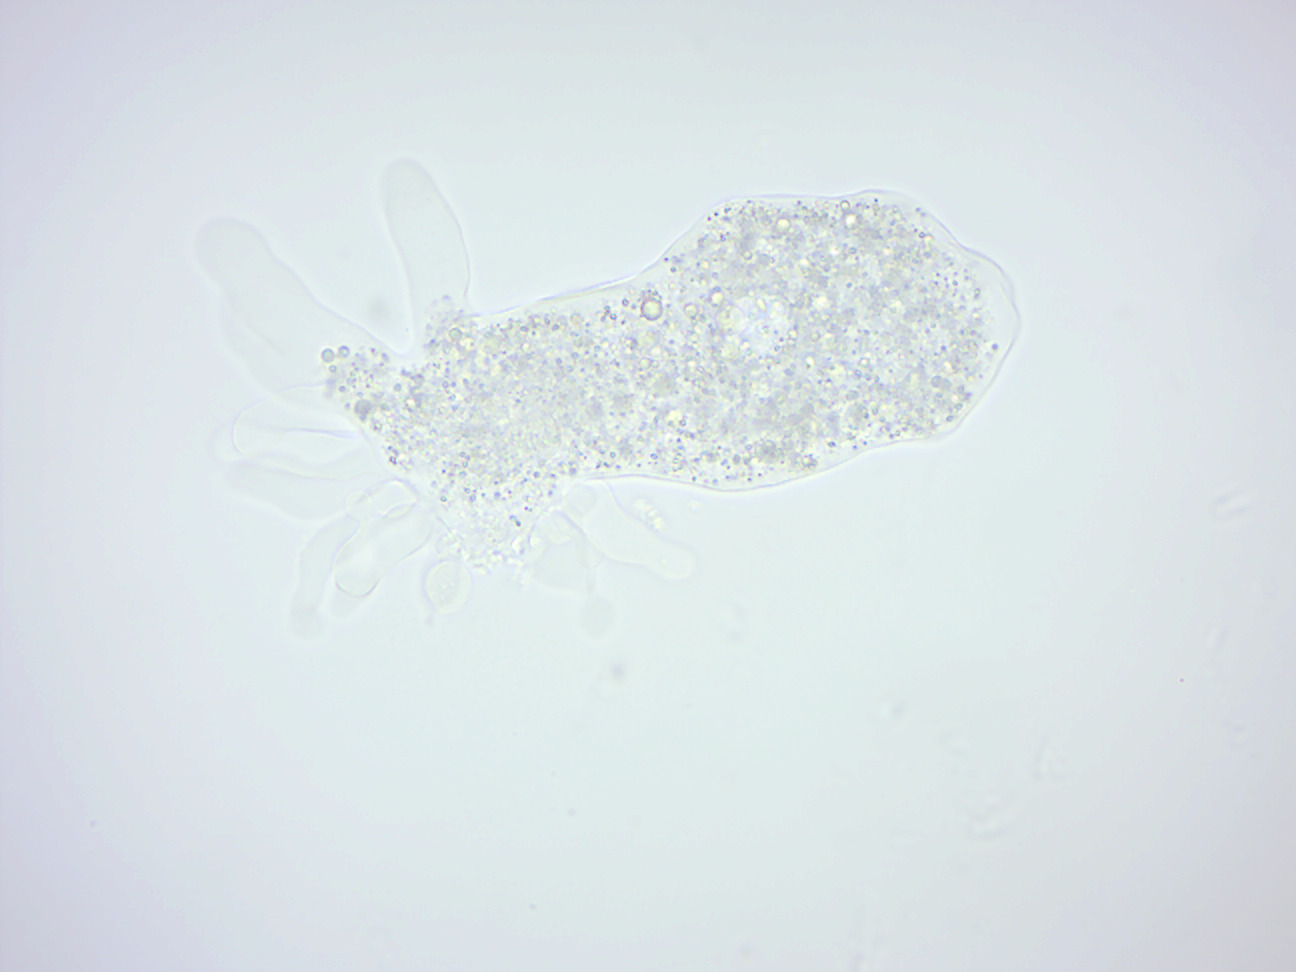
\includegraphics[width=0.7\linewidth]{./figures/protists/Amoeba_proteus} 

}

\caption{Amoeba proteus.}\label{fig:amoeba}
\end{figure}

\subsection{Paramecium caudatum}\label{paramecium-caudatum}

\href{https://en.wikipedia.org/wiki/Paramecium_caudatum}{\emph{Paramecium
caudatum}} (Figure \ref{fig:paramecium}) is a unicellular, ciliate
eukaryote. They can reach 0.25mm in length and are covered with minute
hair-like organelles called cilia. The cilia are used in locomotion and
feeding. P. caudatum feed on bacteria and small eukaryotic cells, such
as yeast and flagellate algae. In hypotonic conditions (freshwater), the
cell absorbs water by osmosis. It regulates osmotic pressure with the
help of bladder-like contractile vacuoles, gathering internal water
through its star-shaped radial canals and expelling the excess through
the plasma membrane. When moving through the water, they follow a spiral
path while rotating on the long axis. Paramecium have two nuclei (a
large macronucleus and a single compact micronucleus). They cannot
survive without the macronucleus and cannot reproduce without the
micro-nucleus. Like all ciliates, Paramecia reproduce asexually, by
binary fission. During reproduction, the macronucleus splits by a type
of amitosis, and the micronuclei undergo mitosis. The cell then divides
transversally, and each new cell obtains a copy of the micronucleus and
the macronucleus. Fission may occur as part of the normal vegetative
cell cycle. Under certain conditions, it may be preceded by
self-fertilization (autogamy), or it may follow conjugation, a sexual
phenomenon in which Paramecia of compatible mating types fuse
temporarily and exchange genetic material. During conjugation, the
micronuclei of each conjugant divide by meiosis and the haploid gametes
pass from one cell to the other. The gametes of each organism then fuse
to form diploid micronuclei. The old macronuclei are destroyed, and new
ones are developed from the new micronuclei. Without the rejuvenating
effects of autogamy or conjugation a Paramecium ages and dies. Only
opposite mating types, or genetically compatible organisms, can unite in
conjugation.

\begin{figure}

{\centering 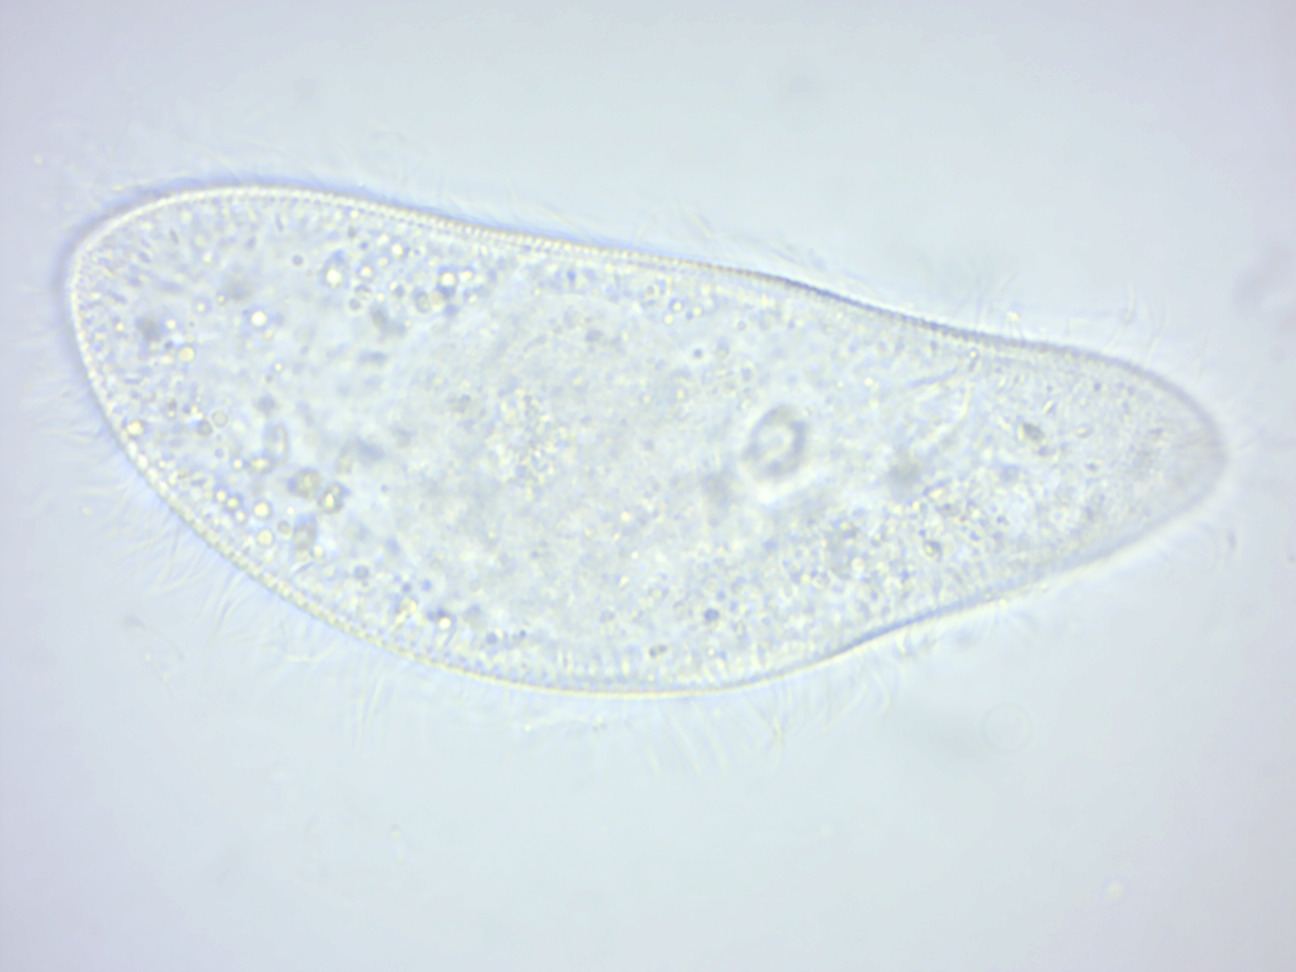
\includegraphics[width=0.7\linewidth]{./figures/protists/Paramecium_caudatum} 

}

\caption{Paramecium caudatum.}\label{fig:paramecium}
\end{figure}

\subsection{Euglena}\label{euglena}

\href{https://en.wikipedia.org/wiki/Euglena}{\emph{Euglena}} (Figure
\ref{fig:euglena}) is a genus of single-celled flagellate eukaryotes. It
is the best known and most widely studied member of the class
Euglenoidea, a diverse group containing some 54 genera and at least 800
species. Species of Euglena are found in fresh and salt waters. They are
often abundant in quiet inland waters where they may bloom in numbers
sufficient to color the surface of ponds and ditches green (E. viridis)
or red (E. sanguinea). When feeding as a heterotroph, Euglena takes in
nutrients by osmotrophy, and can survive without light on a diet of
organic matter, such as beef extract, peptone, acetate, ethanol or
carbohydrates. When there is sufficient sunlight for it to feed by
phototrophy, it uses chloroplasts containing the pigments chlorophyll a
and chlorophyll b to produce sugars by photosynthesis. Euglena's
chloroplasts are surrounded by three membranes, while those of plants
and the green algae (among which earlier taxonomists often placed
Euglena) have only two membranes. This fact has been taken as
morphological evidence that Euglena's chloroplasts evolved from a
eukaryotic green alga. Thus, the intriguing similarities between Euglena
and the plants would have arisen not because of kinship but because of a
secondary endosymbiosis. Molecular phylogenetic analysis has lent
support to this hypothesis, and it is now generally accepted.

\begin{figure}

{\centering 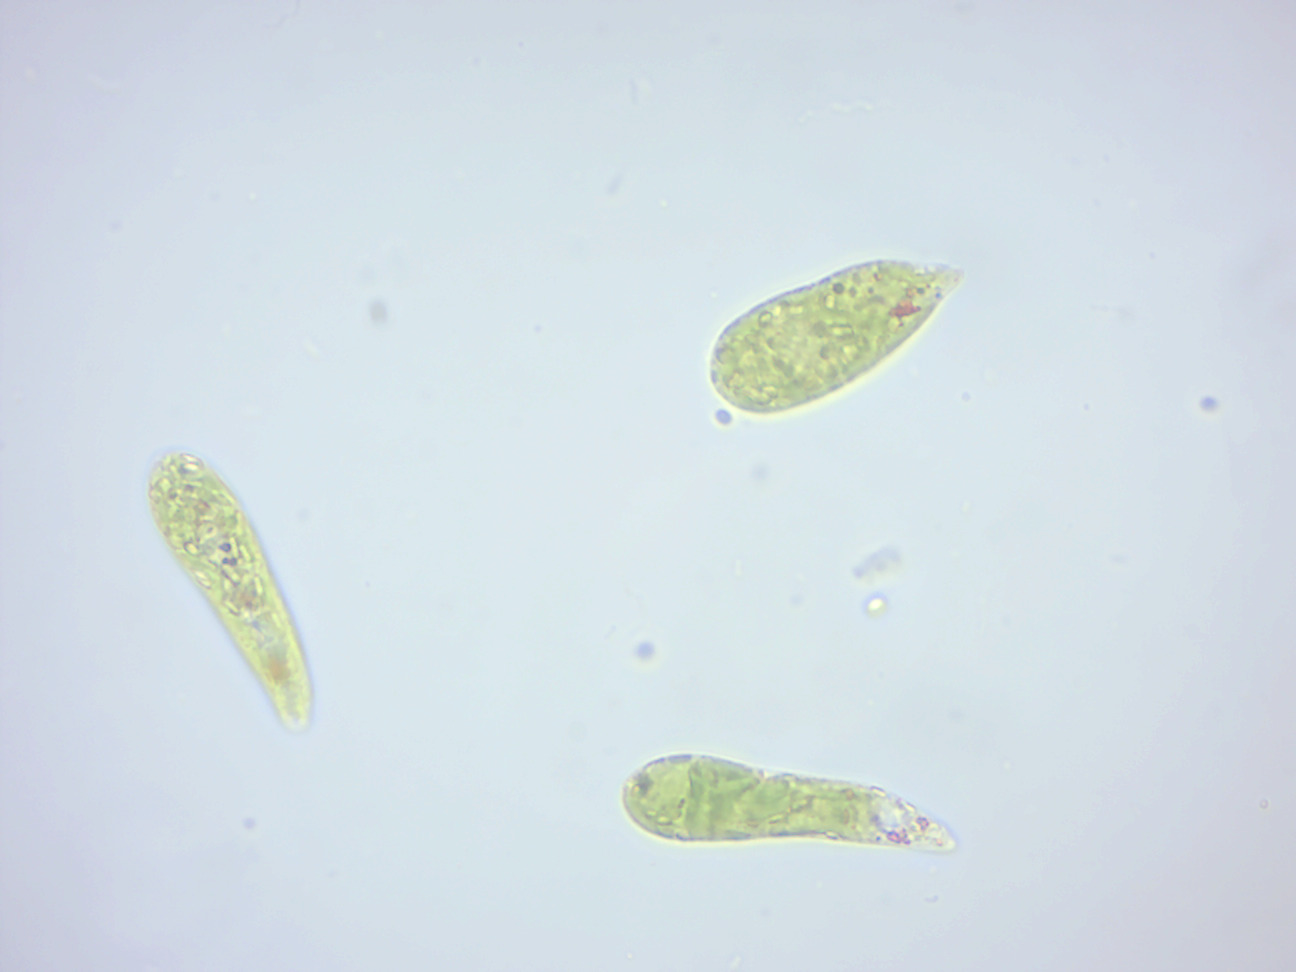
\includegraphics[width=0.7\linewidth]{./figures/protists/euglena} 

}

\caption{Euglena.}\label{fig:euglena}
\end{figure}

\subsection{Peranema}\label{peranema}

\href{https://en.wikipedia.org/wiki/Peranema}{\emph{Peranema}} (Figure
\ref{fig:peranema}) is a genus of free-living flagellate, with more than
20 accepted species, varying in size between 8 and 200 micrometers. They
are found in freshwater lakes, ponds and ditches, and are often abundant
at the bottom of stagnant pools rich in decaying organic material.
Although they belong to the class Euglenoidea, and are morphologically
similar to the green Euglena, Peranema have no chloroplasts, and cannot
feed by autotrophy. Instead, they capture live prey, such as yeast,
bacteria and other flagellates, consuming them with the help of a rigid
feeding apparatus called a ``rod-organ.'' Unlike the green Euglenids,
they lack both an eyespot (stigma), and the paraflagellar body
(photoreceptor) that is normally coupled with that organelle. However,
while Peranema lack a localized photoreceptor, they do possess the
light-sensitive protein rhodopsin, and respond to changes in light with
a characteristic ``curling behavior.''

\begin{figure}

{\centering 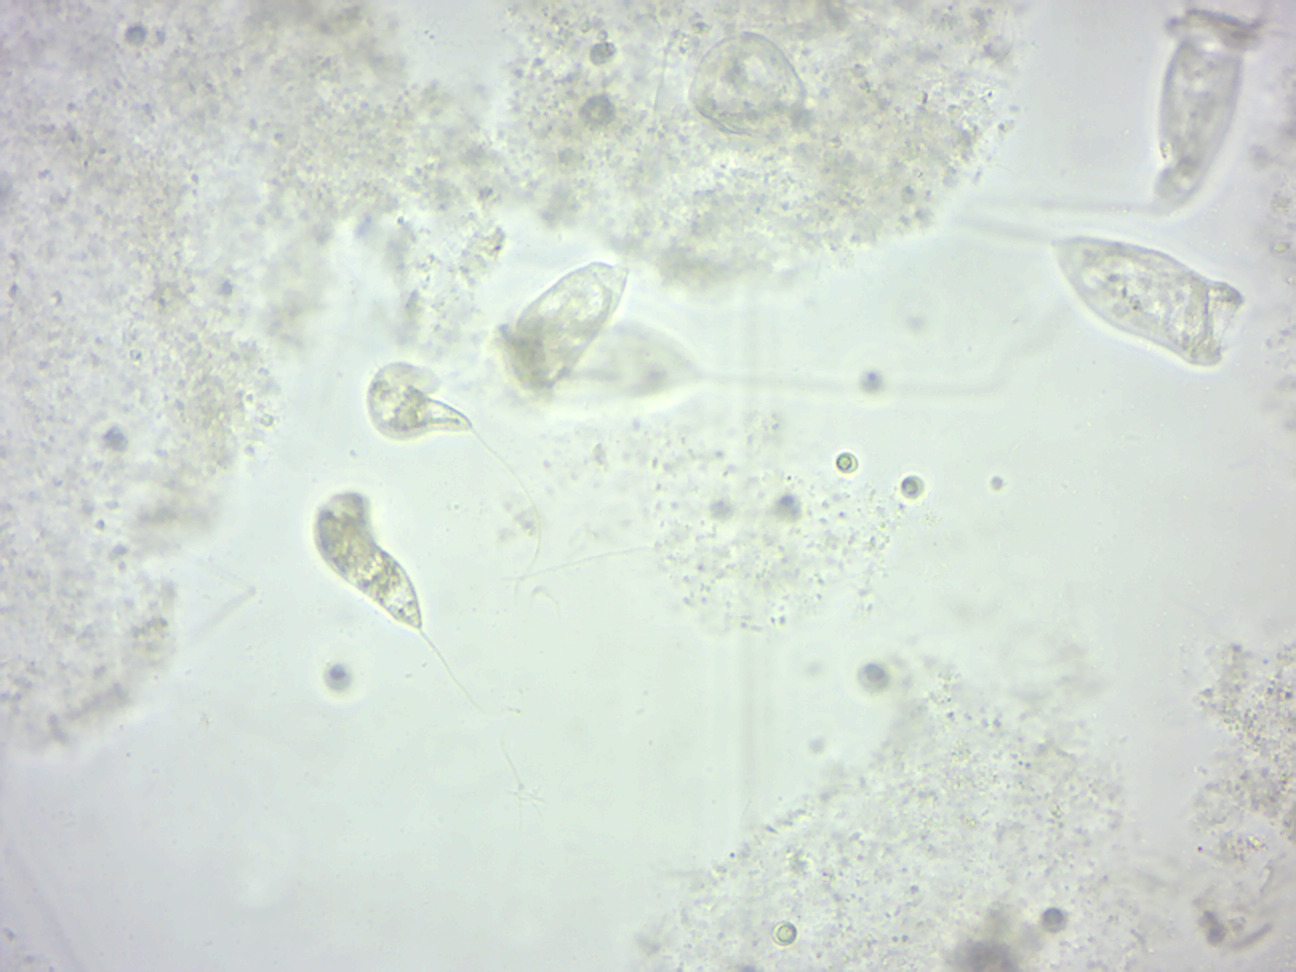
\includegraphics[width=0.7\linewidth]{./figures/protists/peranema} 

}

\caption{Peranema.}\label{fig:peranema}
\end{figure}

\subsection{Chlamydomonas}\label{chlamydomonas}

\href{https://en.wikipedia.org/wiki/Chlamydomonas}{\emph{Chlamydomonas}}
(Figure \ref{fig:chlamydomonaslive}) is a genus of green algae
consisting of unicellular flagellates, found in stagnant water and on
damp soil, in freshwater, seawater, and even in snow as ``snow algae''.
Chlamydomonas is used as a model organism for molecular biology,
especially studies of flagellar motility and chloroplast dynamics,
biogeneses, and genetics. One of the many striking features of
Chlamydomonas is that it contains ion channels, (channelrhodopsins),
that are directly activated by light. These proteins are used in
optogenetics.

\begin{figure}

{\centering 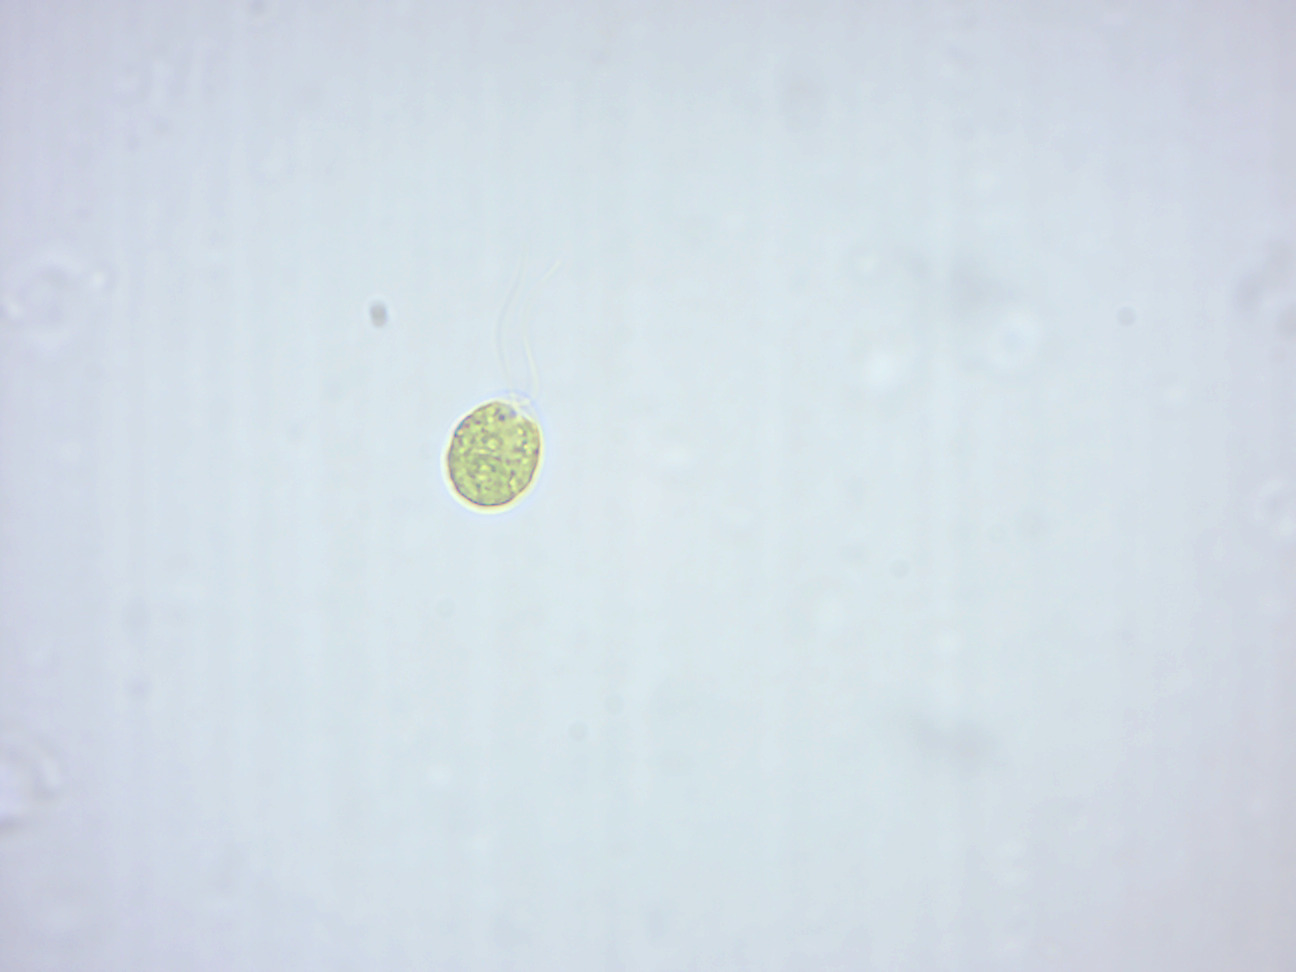
\includegraphics[width=0.7\linewidth]{./figures/protists/chlamydomonas_live} 

}

\caption{Chlamydomonas. Note the flagella.}\label{fig:chlamydomonaslive}
\end{figure}

\subsection{Gymnodinium}\label{gymnodinium}

\href{https://en.wikipedia.org/wiki/Gymnodinium}{\emph{Gymnodinium}} is
a genus of
\href{https://en.wikipedia.org/wiki/Dinoflagellate}{dinoflagellates} It
is one of the few naked dinoflagellates, or species lacking armor
(cellulosic plates). The dinoflagellates (Greek dinos ``whirling'' and
Latin flagellum ``whip, scourge'') are a large group of flagellate
eukaryotes that constitute the phylum Dinoflagellata. Most are marine
plankton, but they are common in freshwater habitats, as well. Their
populations are distributed depending on temperature, salinity, or
depth. Many dinoflagellates are known to be photosynthetic, but a large
fraction of these are in fact mixotrophic, combining photosynthesis with
ingestion of prey (phagotrophy). In terms of number of species,
dinoflagellates form one of the largest groups of marine eukaryotes,
although this group is substantially smaller than the diatoms. Some
species are endosymbionts of marine animals and play an important part
in the biology of coral reefs. Other dinoflagellates are unpigmented
predators on other protozoa, and a few forms are parasitic.

\subsection{Pandorina}\label{pandorina}

\href{https://en.wikipedia.org/wiki/Pandorina}{\emph{Pandorina}} (Figure
\ref{fig:pandorina}) is a genus of green algae composed of 8, 16, or
sometimes 32 cells, held together at their bases to form a sack globular
colony surrounded by mucilage. The cells are ovoid or slightly narrowed
at one end to appear keystone- or pear-shaped. Each cell has two
flagella with two contractile vacuoles at their base, an eyespot, and a
large cup-shaped chloroplast with at least one pyrenoid. The colonies
co-ordinate their flagellar movement to create a rolling, swimming
motion. Pandorina shows the beginnings of the colony polarity and
differentiation seen in Volvox since the anterior cells have larger
eyespots. Asexual reproduction is by simultaneous division of all cells
of the colony to form autocolonies that are liberated by a
gelatinization of the colonial envelope. Sexual reproduction occurs by
division of each cell of the colony into 16-32 zoogametes. Zoogametes
show indications of heterogamy, a slight difference in the size and
motility of the pairs that fuse to form the smooth walled zygote.

\begin{figure}

{\centering 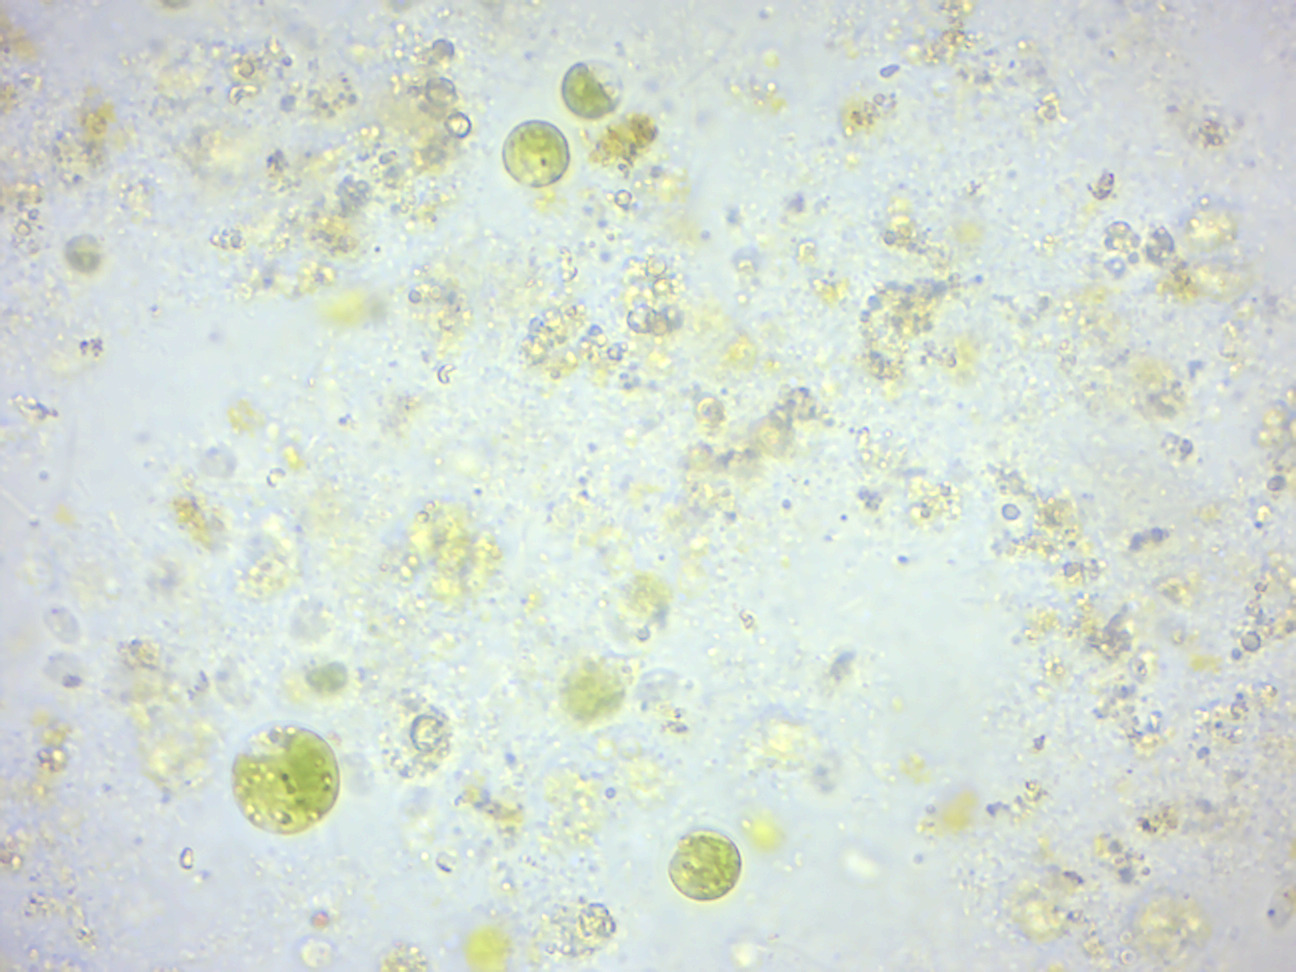
\includegraphics[width=0.7\linewidth]{./figures/protists/Pandorina} 

}

\caption{Pandorina.}\label{fig:pandorina}
\end{figure}

\subsection{Volvox}\label{volvox}

\href{https://en.wikipedia.org/wiki/Volvox}{\emph{Volvox}} (Figure
\ref{fig:volvox}) is a genus of freshwater algae found in ponds and
ditches, even in shallow puddles. It forms spherical colonies of up to
50,000 cells that were first reported by Antonie van Leeuwenhoek in
1700. Volvox diverged from unicellular ancestors approximately 200
million years ago. Each mature Volvox colony is composed of up to
thousands of cells from two differentiated cell types: numerous
flagellate somatic cells and a smaller number of germ cells lacking in
soma that are embedded in the surface of a hollow sphere or coenobium
containing an extracellular matrix made of glycoproteins. Adult somatic
cells comprise a single layer with the flagella facing outward. The
cells swim in a coordinated fashion, with distinct anterior and
posterior poles. The cells have anterior eyespots that enable the colony
to swim towards light. An asexual colony includes both somatic
(vegetative) cells, which do not reproduce, and large, non-motile
gonidia in the interior, which produce new colonies through repeated
division. In sexual reproduction two types of gametes are produced.
Volvox species can be monoecious or dioecious. Male colonies release
numerous sperm packets, while in female colonies single cells enlarge to
become oogametes, or eggs. Volvox is facultatively sexual and can
reproduce both sexually and asexually. The switch from asexual to sexual
reproduction can be triggered by environmental conditions and by the
production of a sex-inducing pheremone. Desiccation-resistant diploid
zygotes are produced following successful fertilization.

\begin{figure}

{\centering 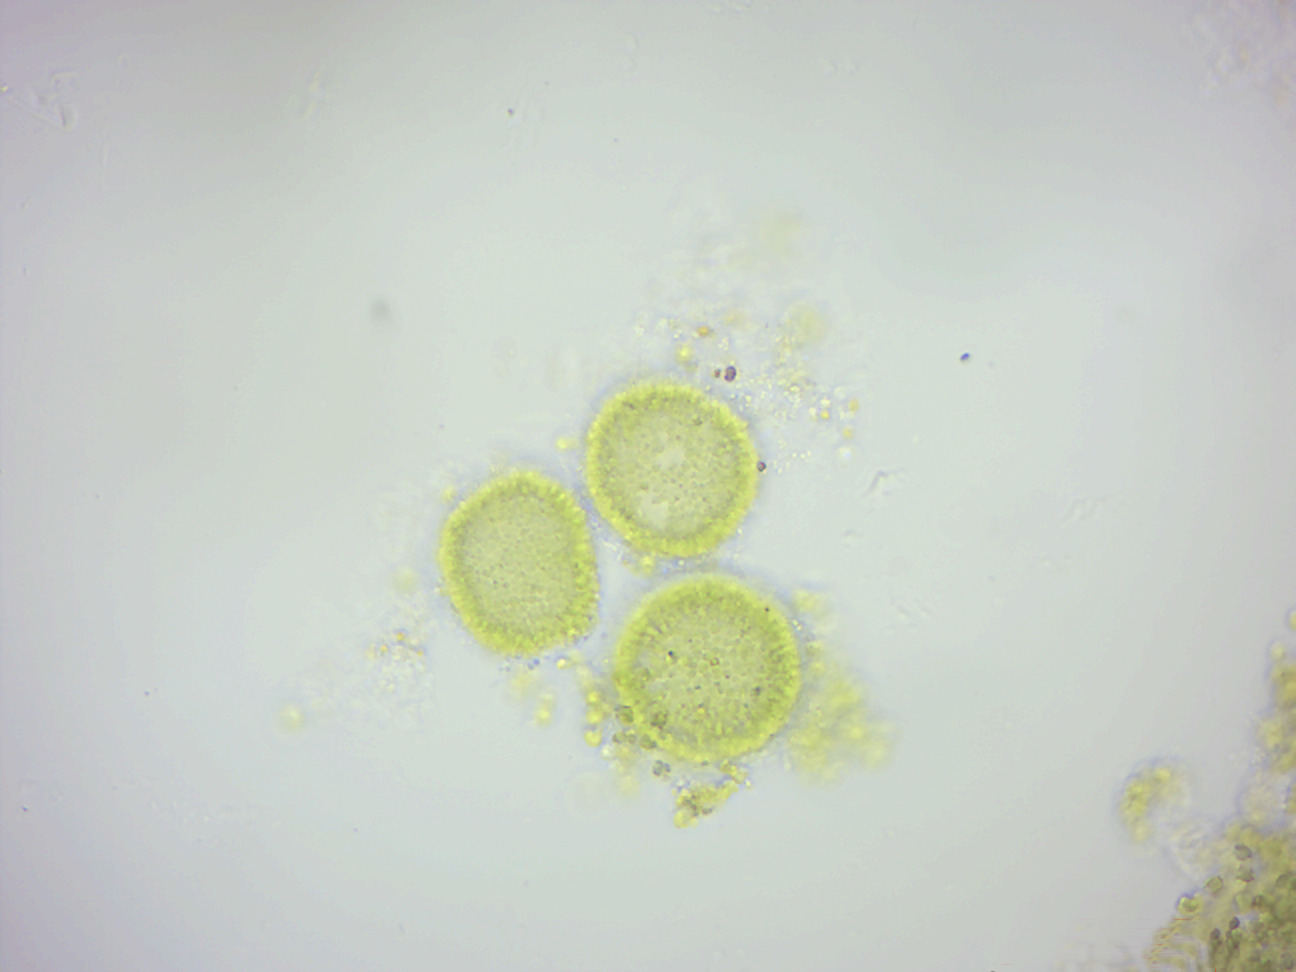
\includegraphics[width=0.7\linewidth]{./figures/protists/Volvox} 

}

\caption{Volvox.}\label{fig:volvox}
\end{figure}

\subsection{Oedogonium}\label{oedogonium}

\href{https://en.wikipedia.org/wiki/Oedogonium}{\emph{Oedogonium}}
(Figure \ref{fig:oedogonium}) is a genus of filamentous green algae,
with unbranched filaments that are one cell thick. Oedogonium can be
free-floating, though it is usually attached to aquatic plants by a
holdfast. It appears greenish and inhabits calm, fresh water. Oedogonium
can reproduce asexually by fragmentation of the filaments, through some
other types of non-motile spores, and also through zoospores, which have
many flagella. These develop in a zoosporangium cell, one zoospore per
zoosporangium. After settling and losing its flagella, a zoospore grows
into a filament. Oedogonium can also reproduce sexually. Its sexual life
cycle is haplontic, i.e., the zygote undergoes meiosis. Antheridia
produce and release sperm, and oogonia produce and release an egg,. The
egg and sperm then fuse and form a zygote which is diploid (2n). The
zygote then undergoes meiosis to produce the filamentous green alga
which is haploid (1n).

\begin{figure}

{\centering 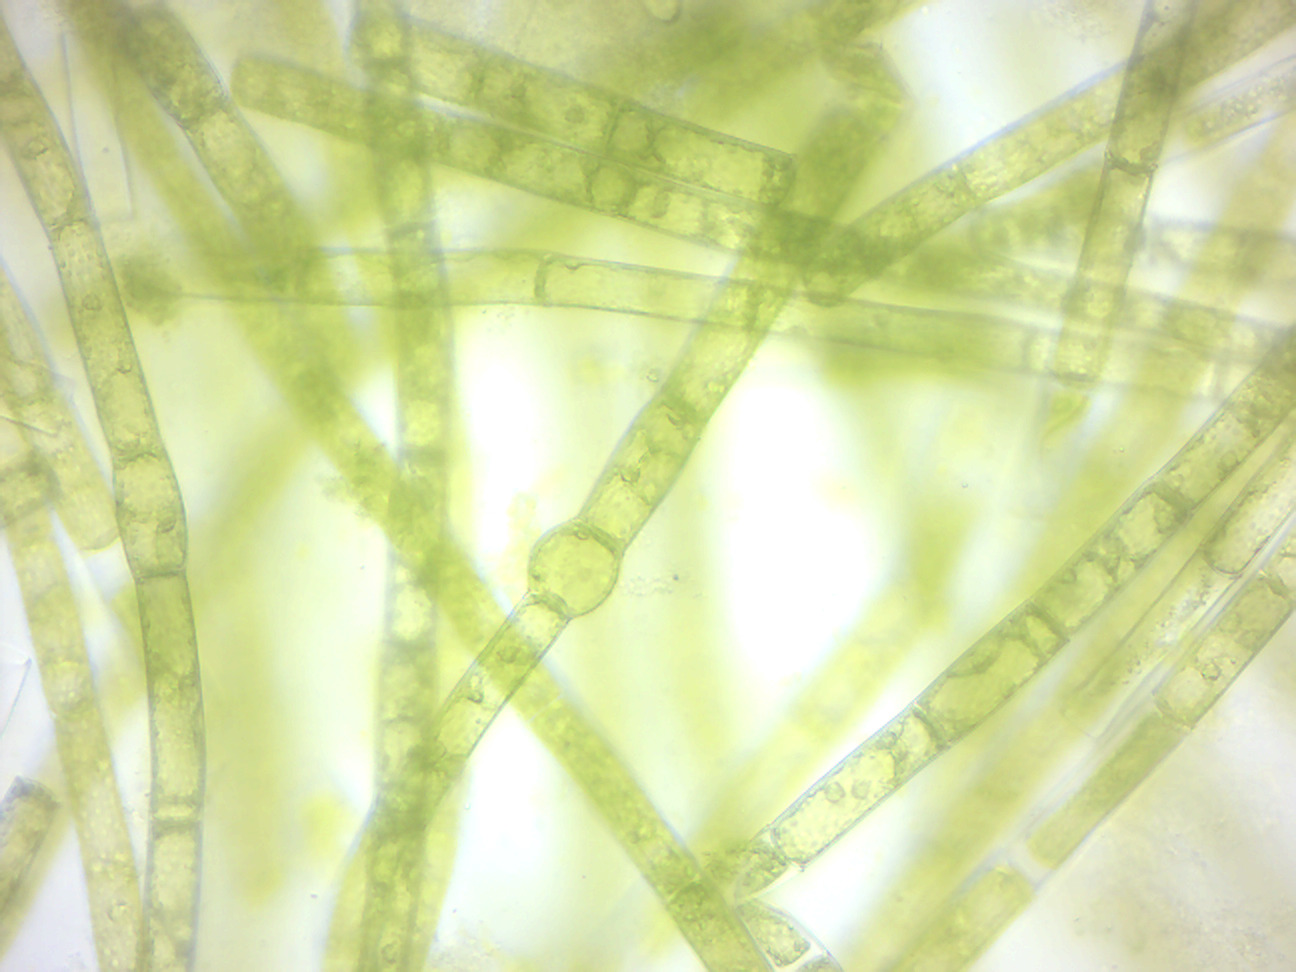
\includegraphics[width=0.7\linewidth]{./figures/protists/oedogonium} 

}

\caption{Oedogonium.}\label{fig:oedogonium}
\end{figure}

\subsection{Spirogyra}\label{spirogyra}

\href{https://en.wikipedia.org/wiki/Spirogyra}{\emph{Spirogyra}} (Figure
\ref{fig:spiro}; common names include water silk, mermaid's tresses, and
blanket weed) is a genus of filamentous chlorophyte green algae of the
order Zygnematales, named for the helical or spiral arrangement of the
chloroplasts that is diagnostic of the genus. It is commonly found in
freshwater areas, and there are more than 400 species of Spirogyra in
the world. Spirogyra measures approximately 10 to 100 μm in width and
may grow to several centimeters in length. Spirogyra can reproduce both
sexually and asexually. In vegetative reproduction, fragmentation takes
place, and Spirogyra simply undergoes the intercalary mitosis to form
new filaments. Sexual Reproduction is of two types: 1. Scalariform
conjugation requires association of two different filaments lined side
by side either partially or throughout their length. One cell each from
opposite lined filaments emits tubular protuberances known as
conjugation tubes, which elongate and fuse, to make a passage called the
conjugation canal. The cytoplasm of the cell acting as the male travels
through this tube and fuses with the female cytoplasm, and the gametes
fuse to form a zygospore. 2. In lateral conjugation, gametes are formed
in a single filament. Two adjoining cells near the common transverse
wall give out protuberances known as conjugation tubes, which further
form the conjugation canal upon contact. The male cytoplasm migrates
through the conjugation canal, fusing with the female. The rest of the
process proceeds as in scalariform conjugation. The essential difference
is that scalariform conjugation occurs between two filaments and lateral
conjugation occurs between two adjacent cells on the same filament.

\begin{figure}

{\centering 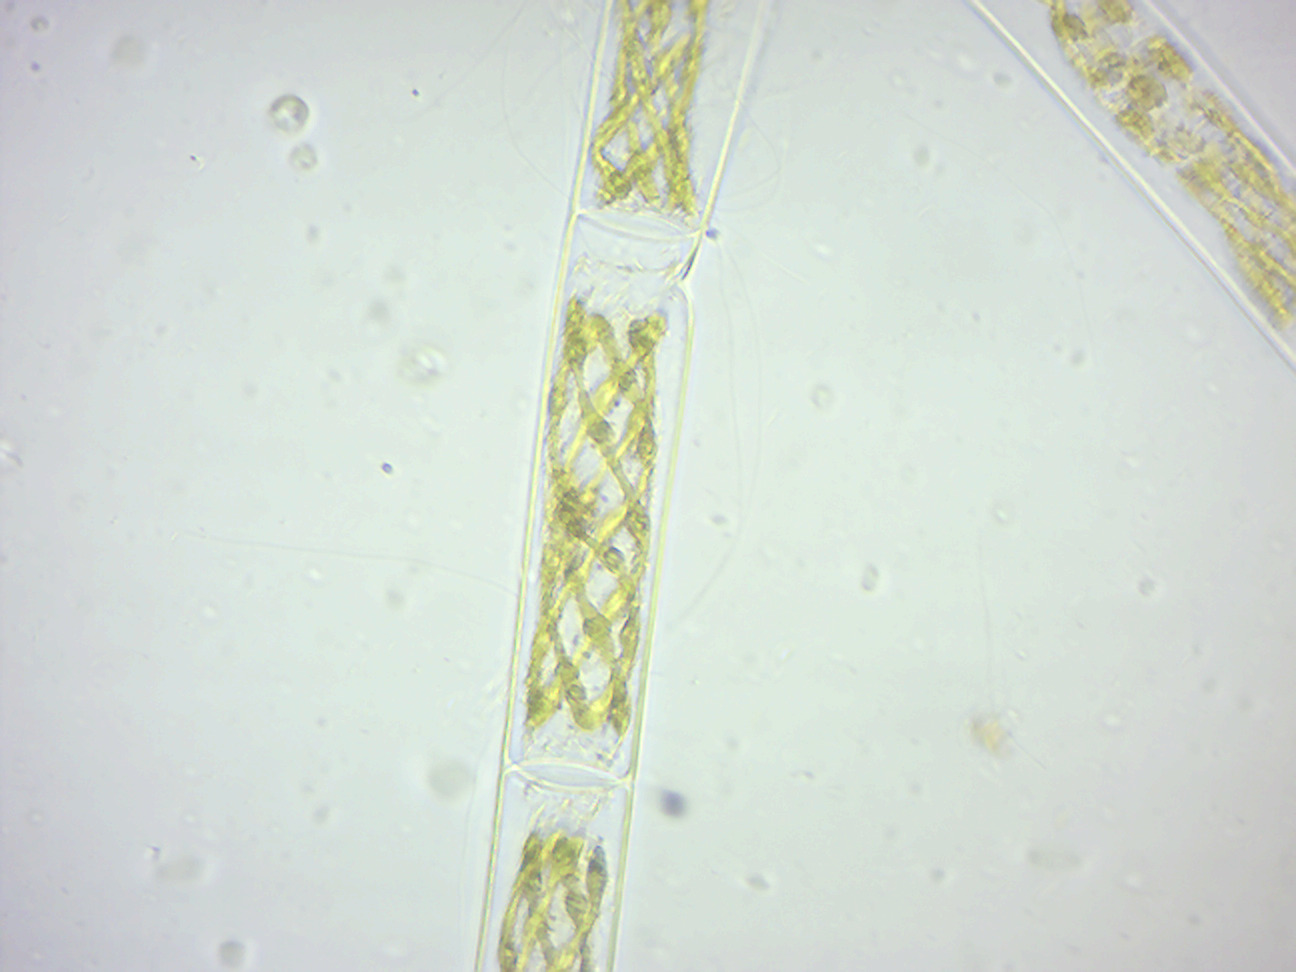
\includegraphics[width=0.7\linewidth]{./figures/protists/Spirogyra} 

}

\caption{Spirogyra.}\label{fig:spiro}
\end{figure}

\section{View Prepared Slides}\label{view-prepared-slides-3}

\subsection{Amoeba proteus (Figure
\ref{fig:amoebaprepared})}\label{amoeba-proteus-figure-reffigamoebaprepared}

\begin{figure}

{\centering 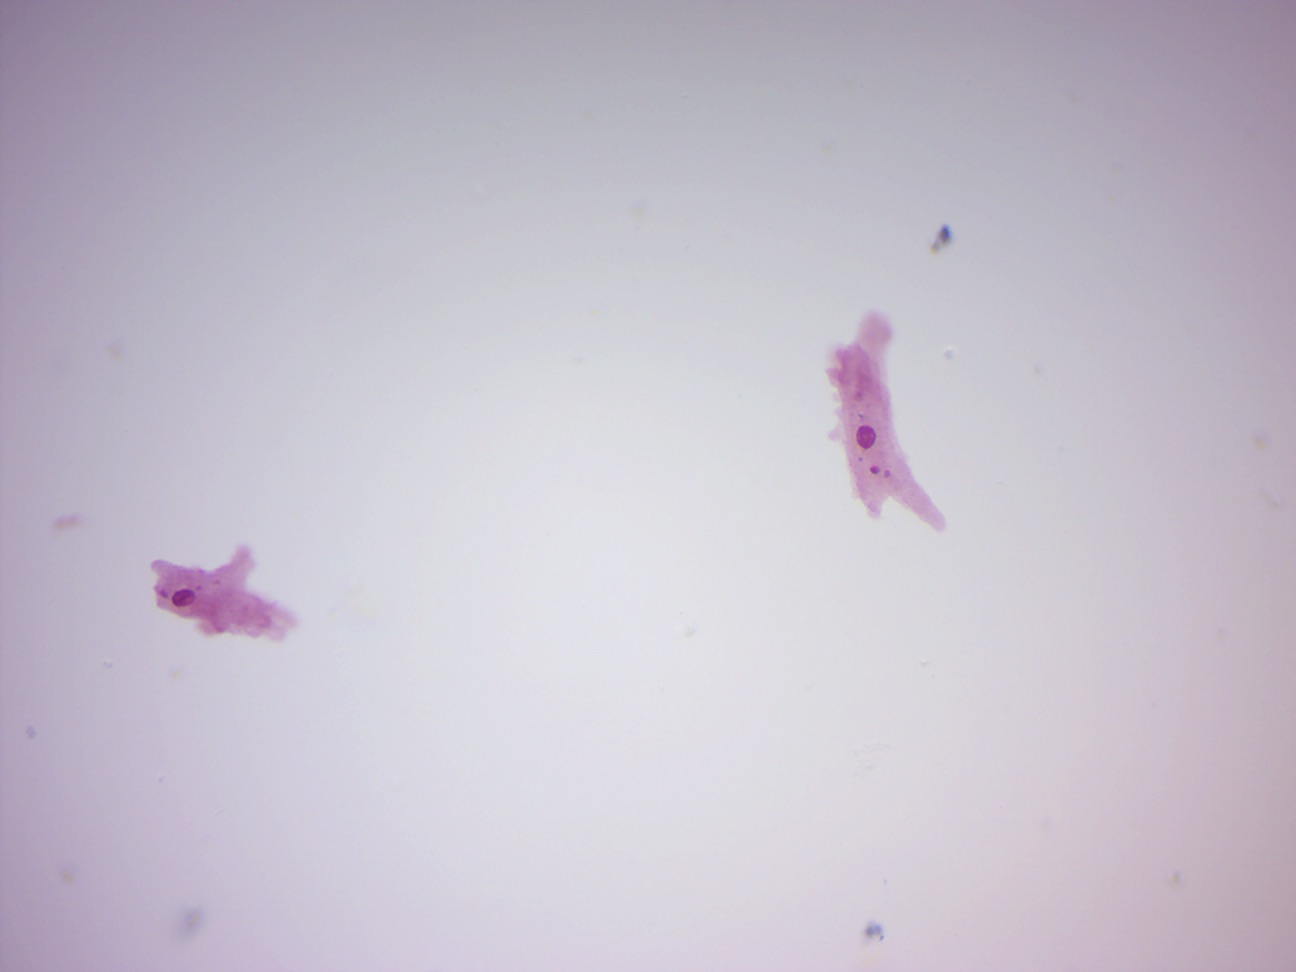
\includegraphics[width=0.7\linewidth]{./figures/protists/Amoeba_proteus_prepared} 

}

\caption{Amoeba proteus.}\label{fig:amoebaprepared}
\end{figure}

\subsection{Paramecium 4 types of protista (Figure
\ref{fig:fourtypes})}\label{paramecium-4-types-of-protista-figure-reffigfourtypes}

\begin{figure}

{\centering 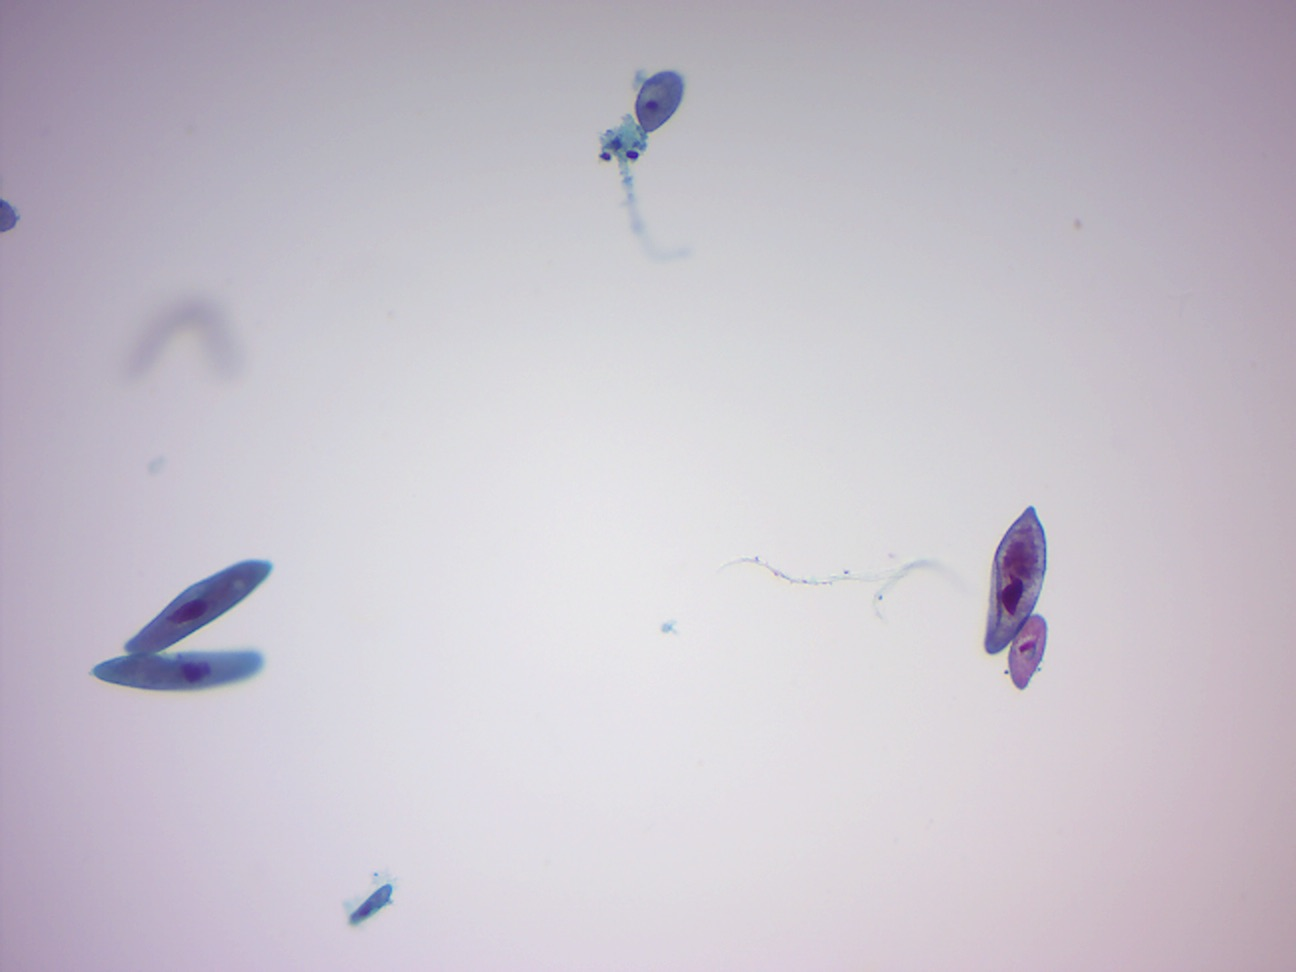
\includegraphics[width=0.7\linewidth]{./figures/protists/Four_types_protista} 

}

\caption{Paramecia and other protists.}\label{fig:fourtypes}
\end{figure}

\subsection{Paramecium caudatum (Figure
\ref{fig:parameciumprepared})}\label{paramecium-caudatum-figure-reffigparameciumprepared}

\begin{figure}

{\centering 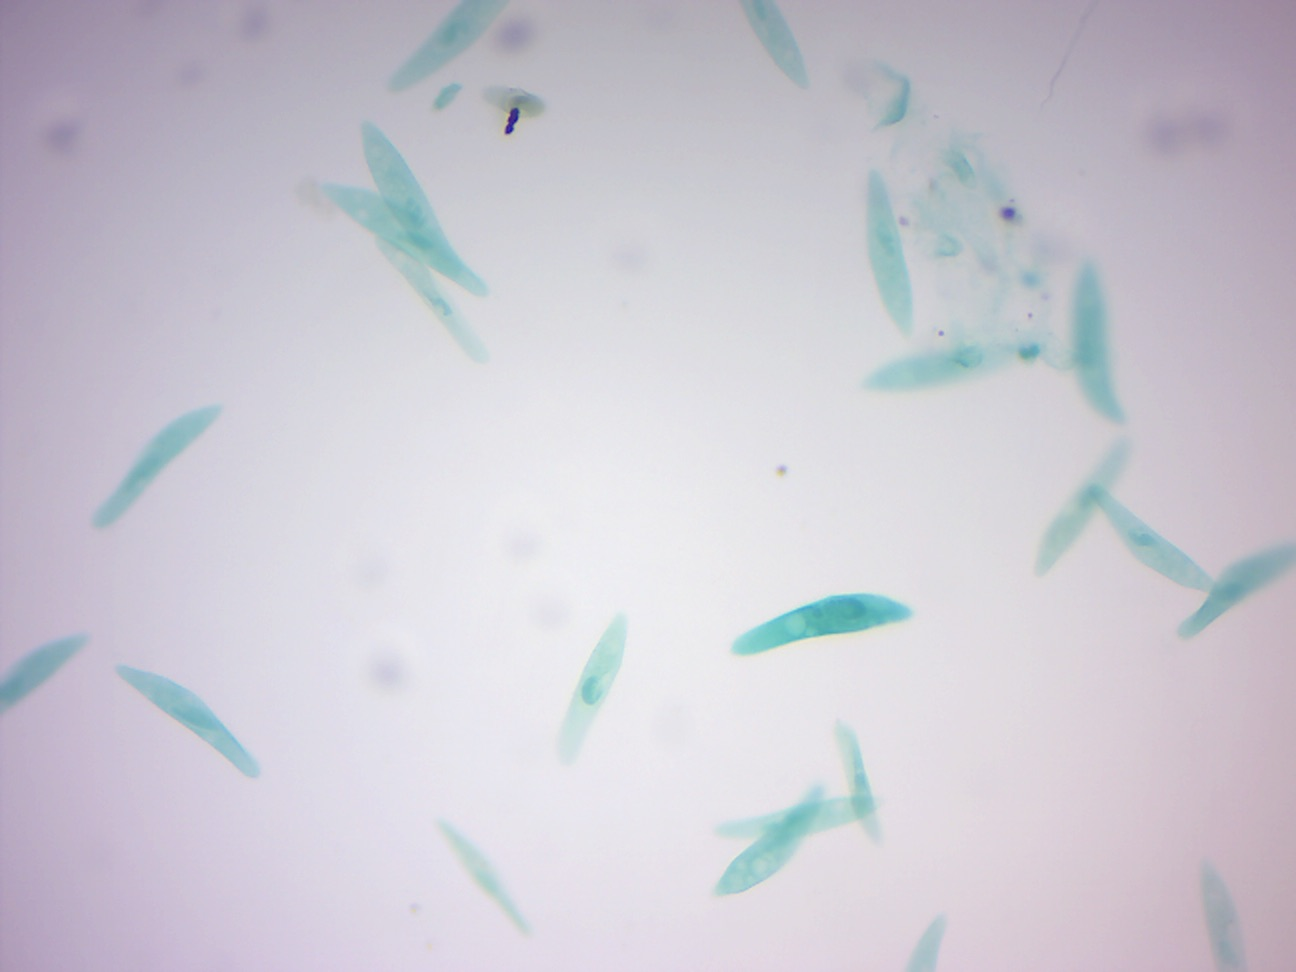
\includegraphics[width=0.7\linewidth]{./figures/protists/Paramecium_prepared} 

}

\caption{Paramecium.}\label{fig:parameciumprepared}
\end{figure}

\subsection{Paramecium in conjugation (Figure
\ref{fig:conjugation})}\label{paramecium-in-conjugation-figure-reffigconjugation}

\begin{figure}

{\centering 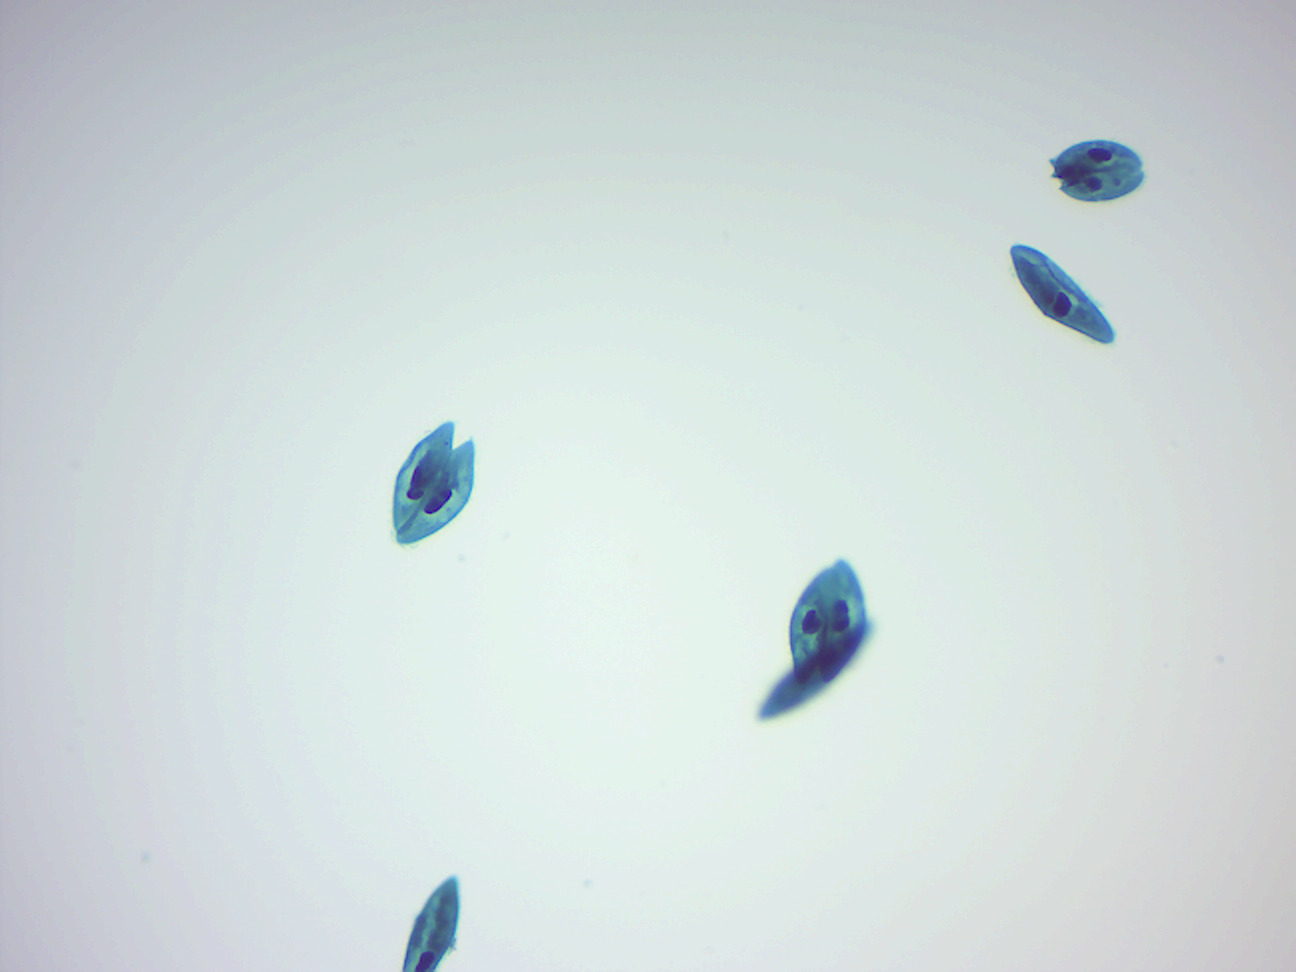
\includegraphics[width=0.7\linewidth]{./figures/protists/paramecium_conjugation} 

}

\caption{Paramecium in conjugation.}\label{fig:conjugation}
\end{figure}

\subsection{Euglena (Figure
\ref{fig:euglenaprepared})}\label{euglena-figure-reffigeuglenaprepared}

\begin{figure}

{\centering 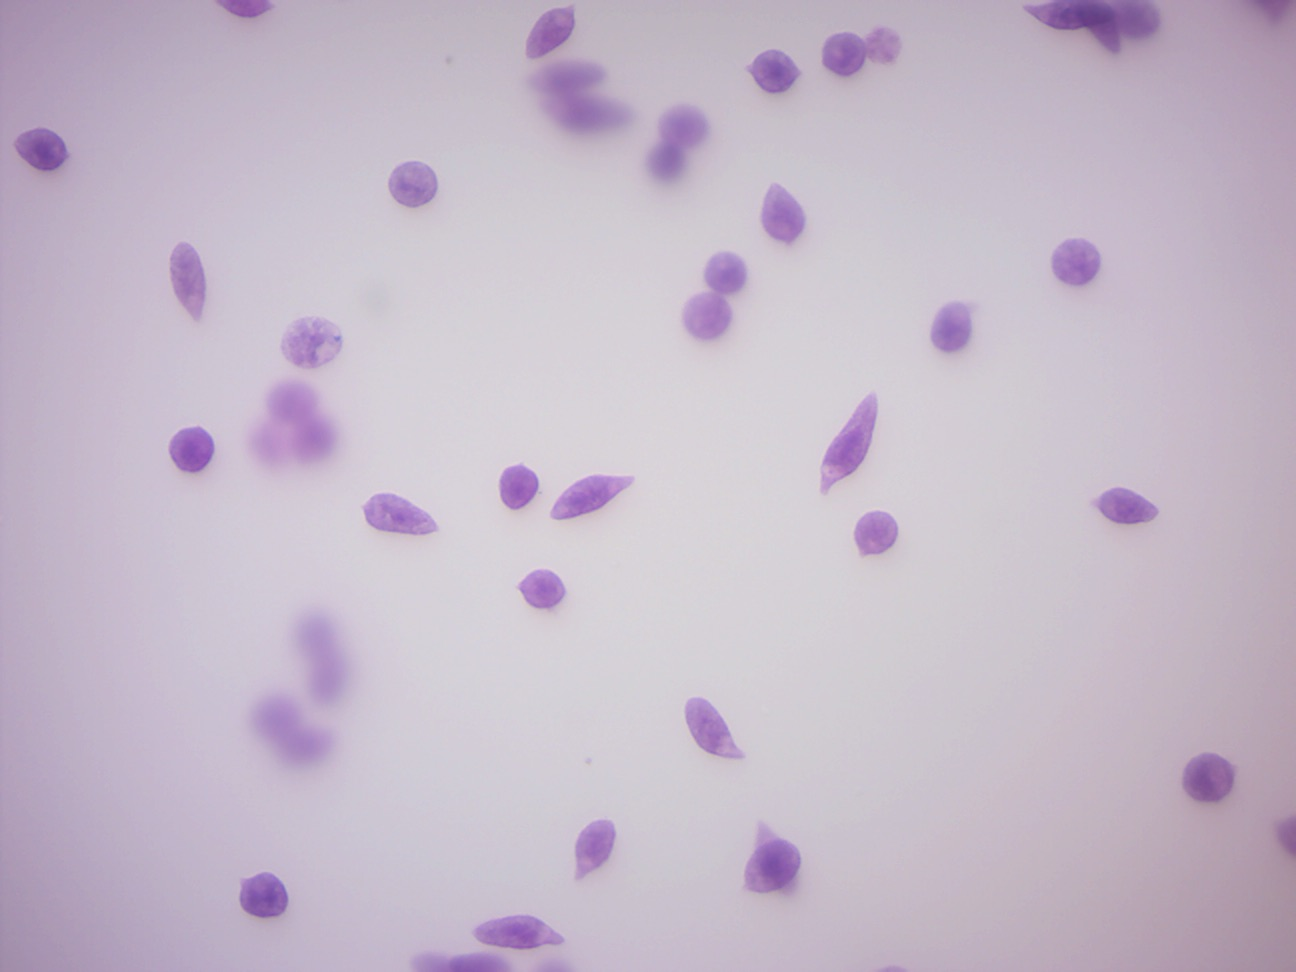
\includegraphics[width=0.7\linewidth]{./figures/protists/Euglena_prepared} 

}

\caption{Euglena.}\label{fig:euglenaprepared}
\end{figure}

\subsection{Dinoflagellate (Figure
\ref{fig:dinoflagellateprepared})}\label{dinoflagellate-figure-reffigdinoflagellateprepared}

\begin{figure}

{\centering 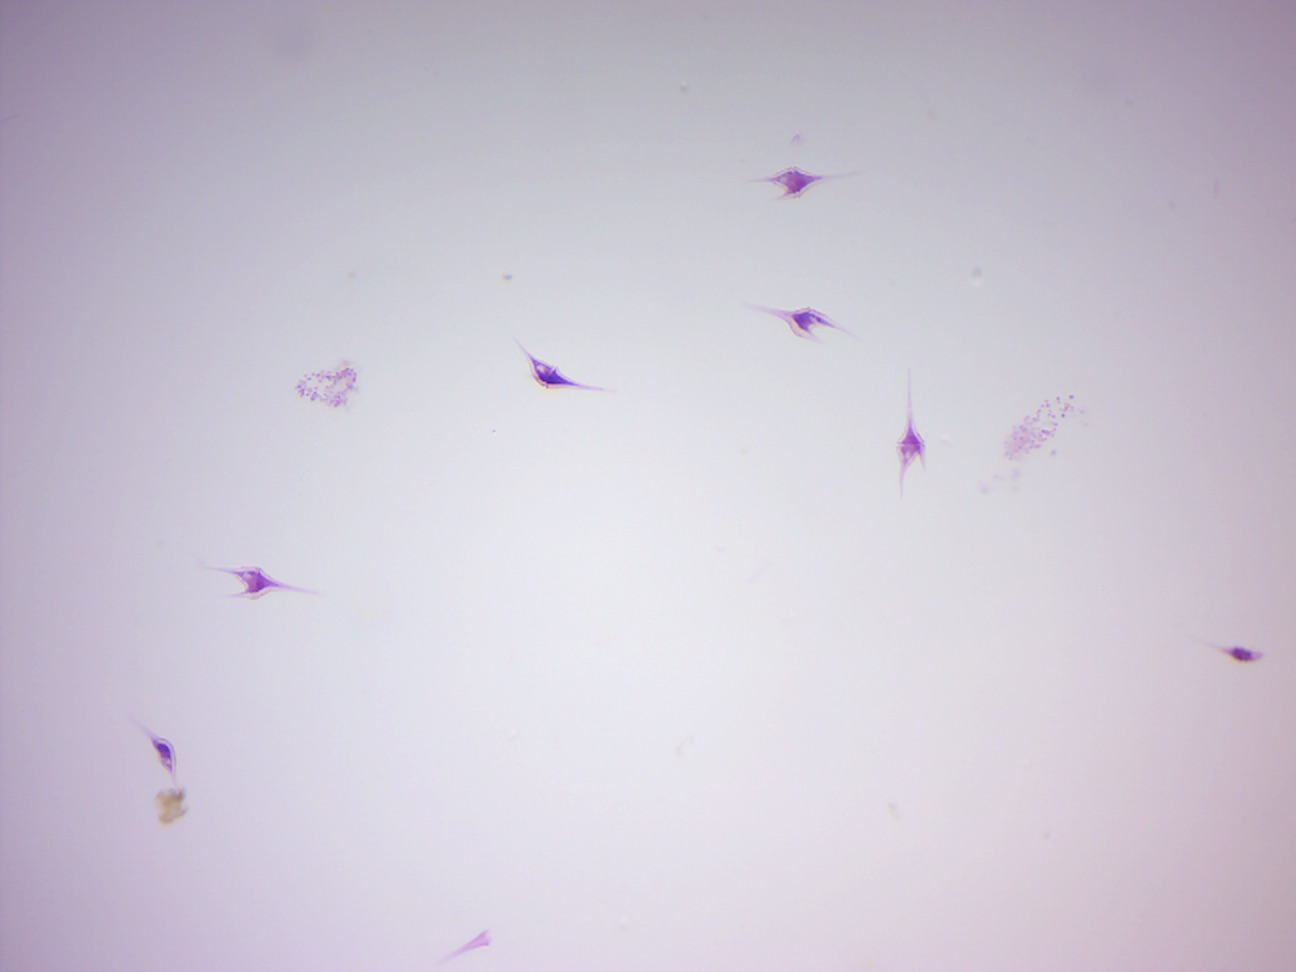
\includegraphics[width=0.7\linewidth]{./figures/protists/Dinoflagellates_prepared} 

}

\caption{Dinoflagellates.}\label{fig:dinoflagellateprepared}
\end{figure}

\subsection{Ceratium (Figure
\ref{fig:ceratium})}\label{ceratium-figure-reffigceratium}

\begin{figure}

{\centering 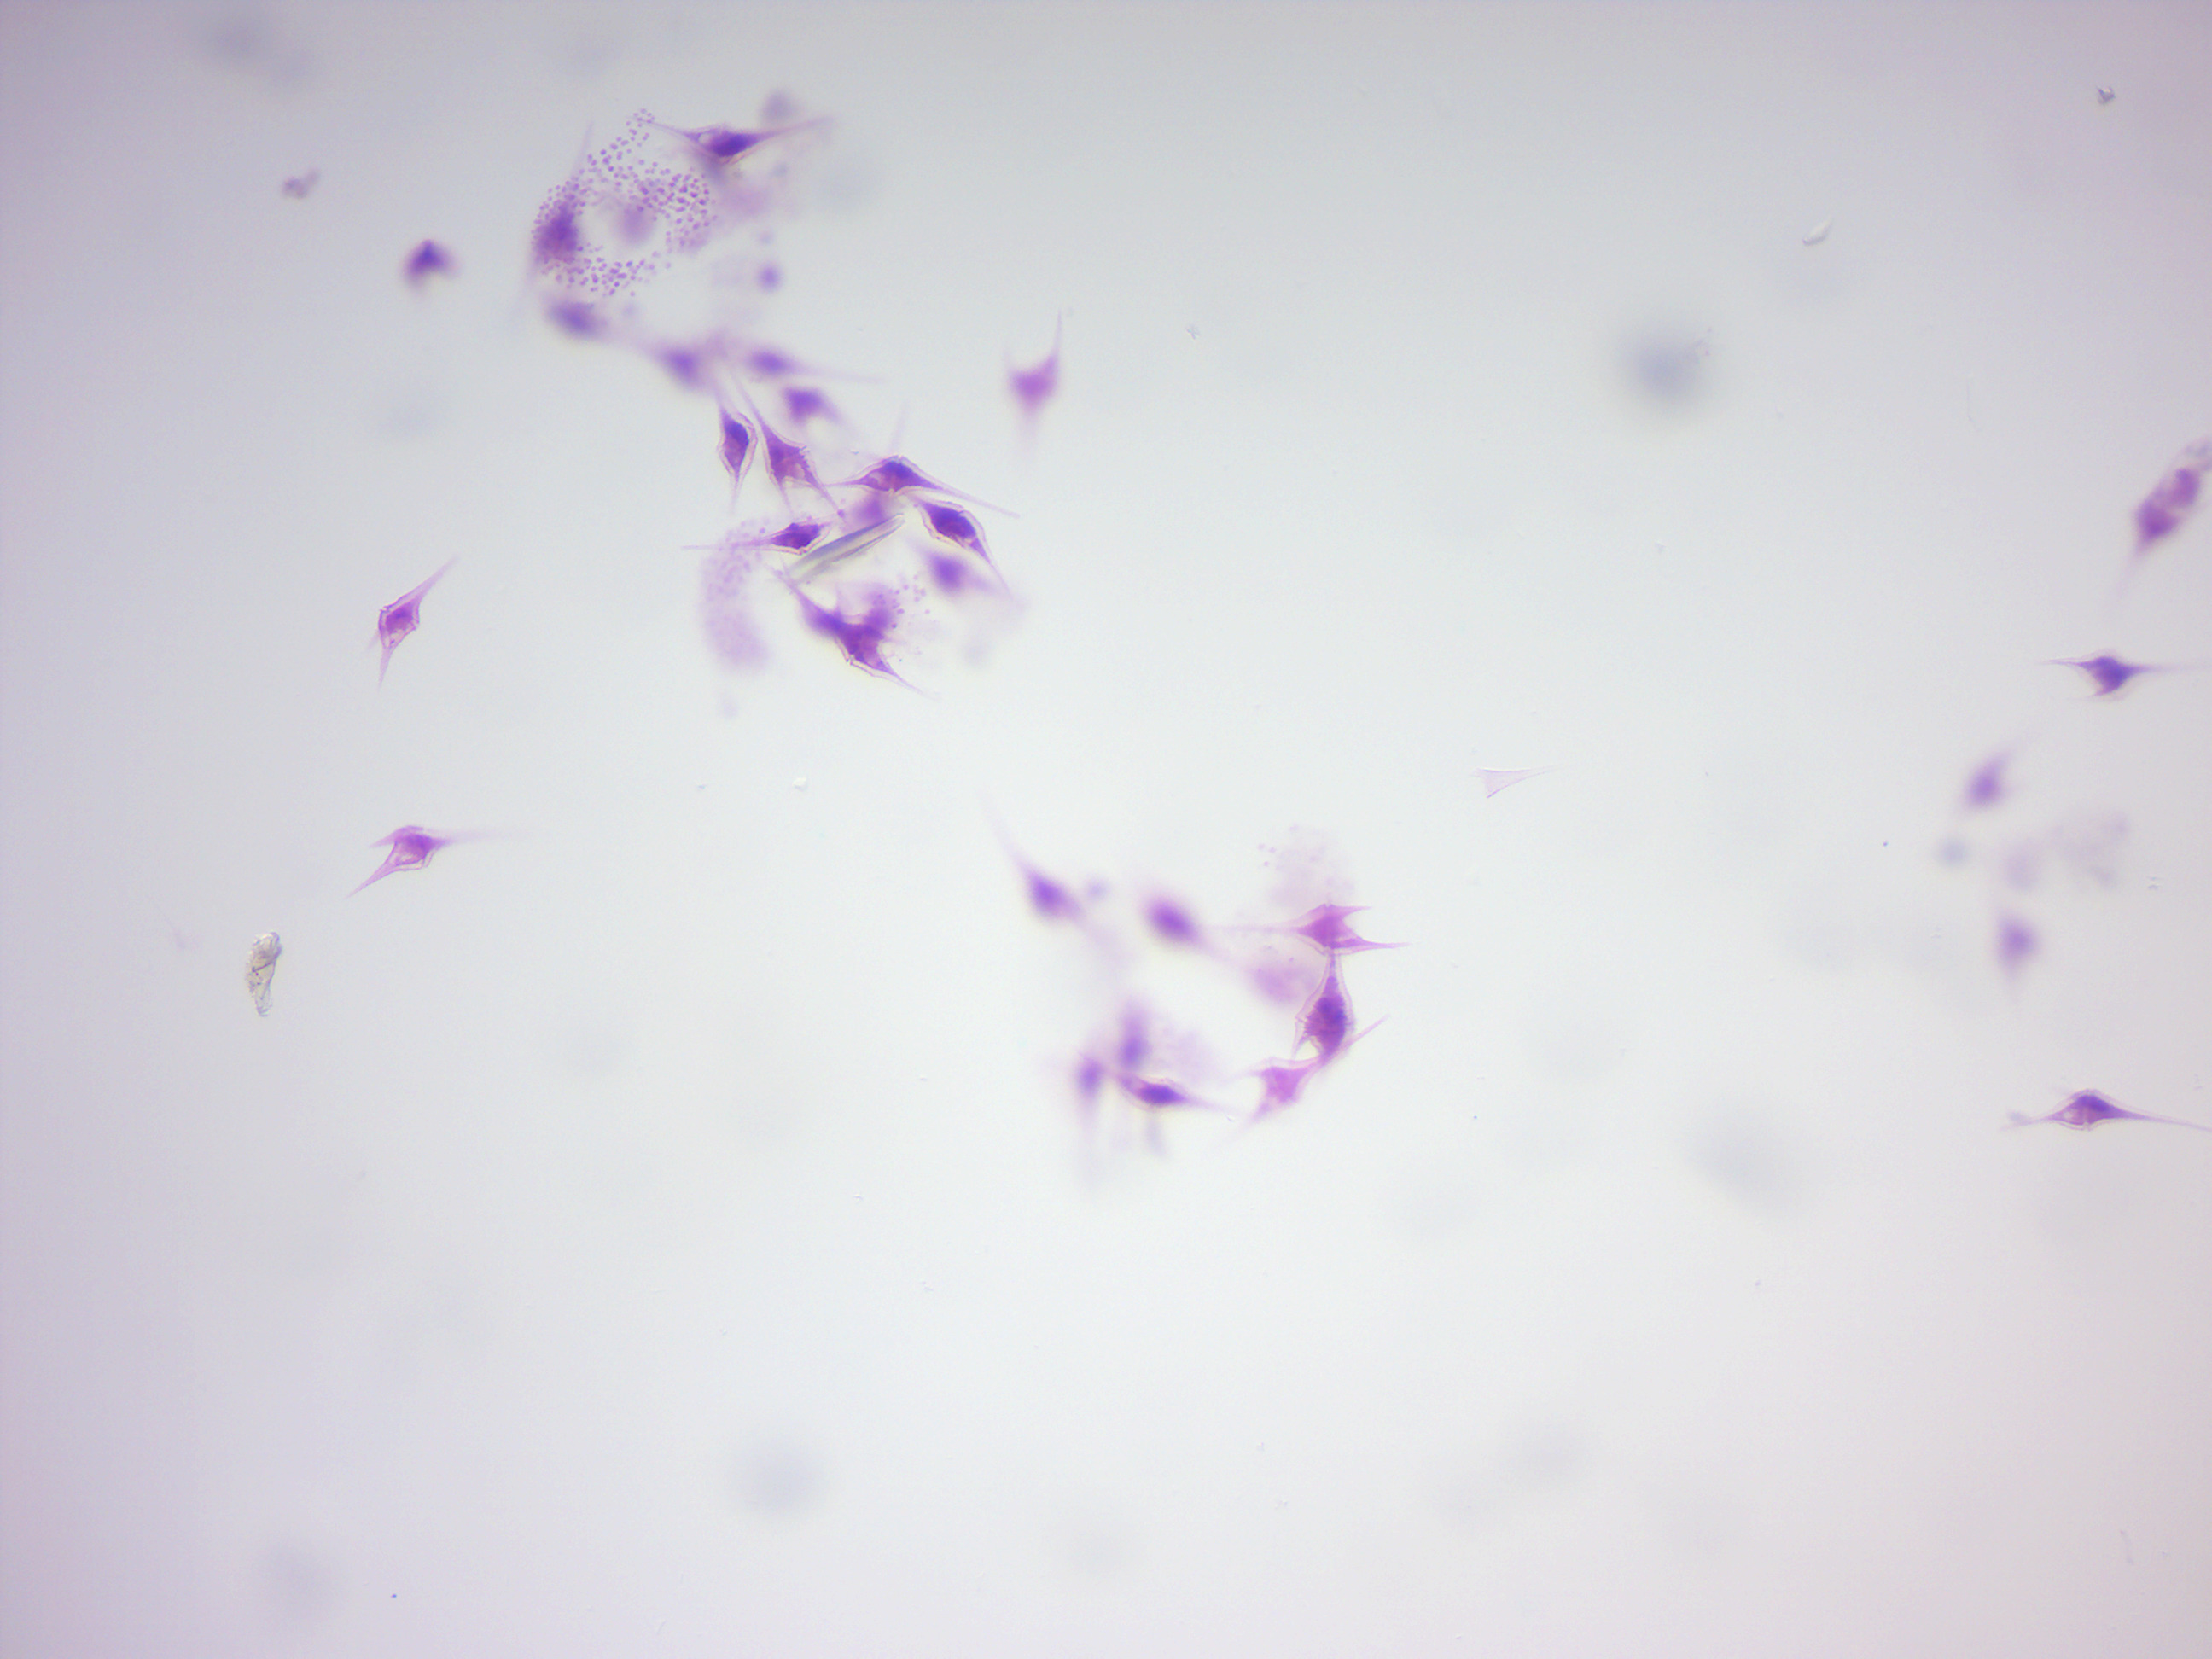
\includegraphics[width=0.7\linewidth]{./figures/protists/ceratium} 

}

\caption{Ceratium, a dinoflagellate.}\label{fig:ceratium}
\end{figure}

\subsection{Peridinium (Figure
\ref{fig:peridinium})}\label{peridinium-figure-reffigperidinium}

\begin{figure}

{\centering 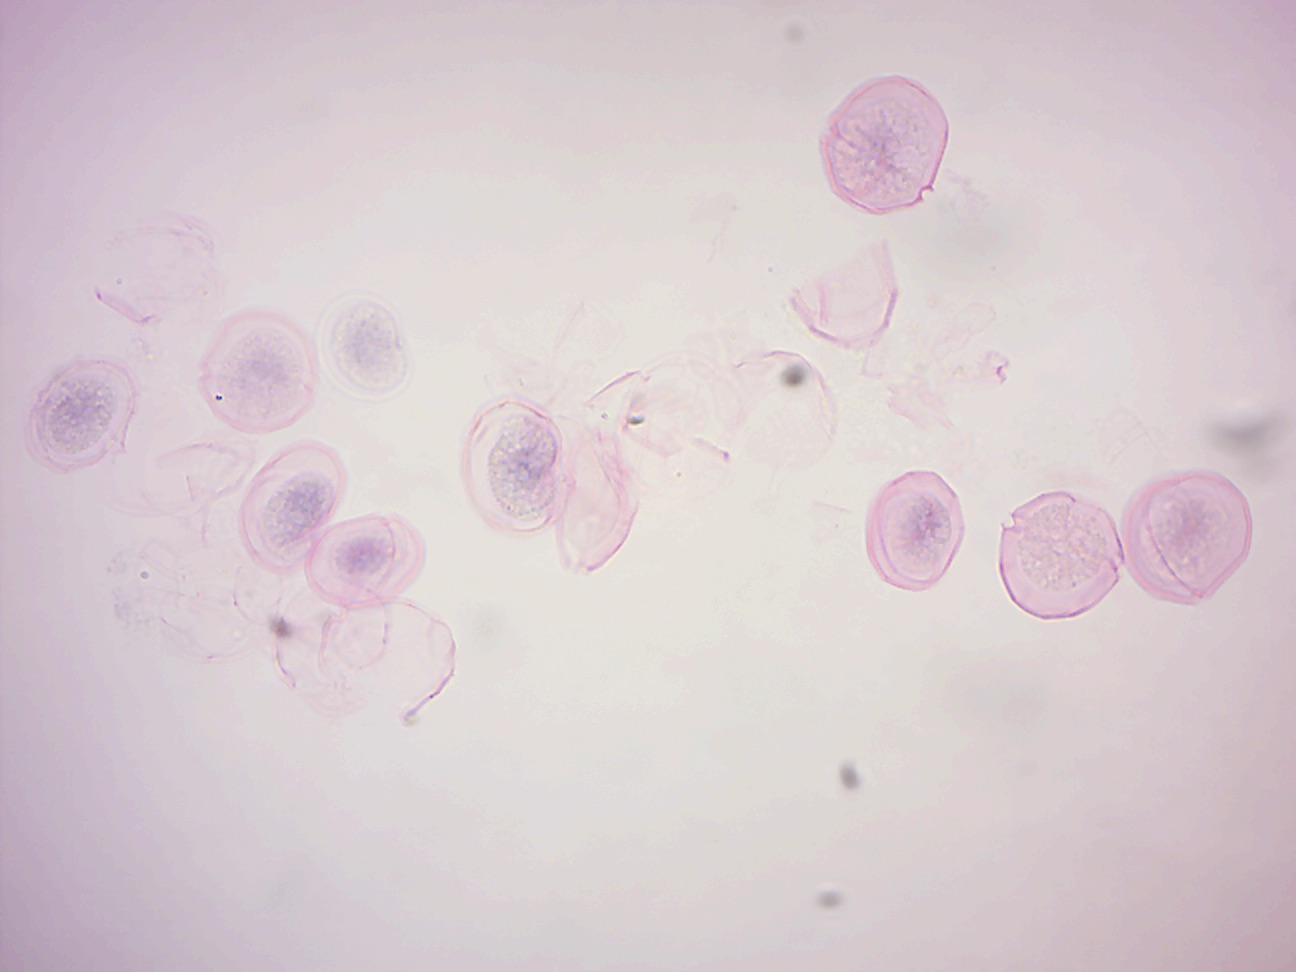
\includegraphics[width=0.7\linewidth]{./figures/protists/Peridinium} 

}

\caption{Peridinium, a dinoflagellate.}\label{fig:peridinium}
\end{figure}

\subsection{Foraminifera}\label{foraminifera}

\href{https://en.wikipedia.org/wiki/Foraminifera}{\emph{Foraminifera}}
(Figure \ref{fig:foraminifera}; Latin meaning hole bearers; informally
called ``forams'') are members of a phylum or class of amoeboid protists
characterized by: streaming granular ectoplasm for catching food and
other uses; and commonly an external shell (called a ``test'') of
diverse forms and materials. Most foraminifera are marine, the majority
of which live on or within the seafloor sediment (i.e., are benthic),
while a smaller variety float in the water column at various depths
(i.e., are planktonic). These shells are commonly made of calcium
carbonate (CaCO\textsubscript{3}) or agglutinated sediment particles.
Over 50,000 species are recognized, both living (10,000) and fossil
(40,000).

\begin{figure}

{\centering 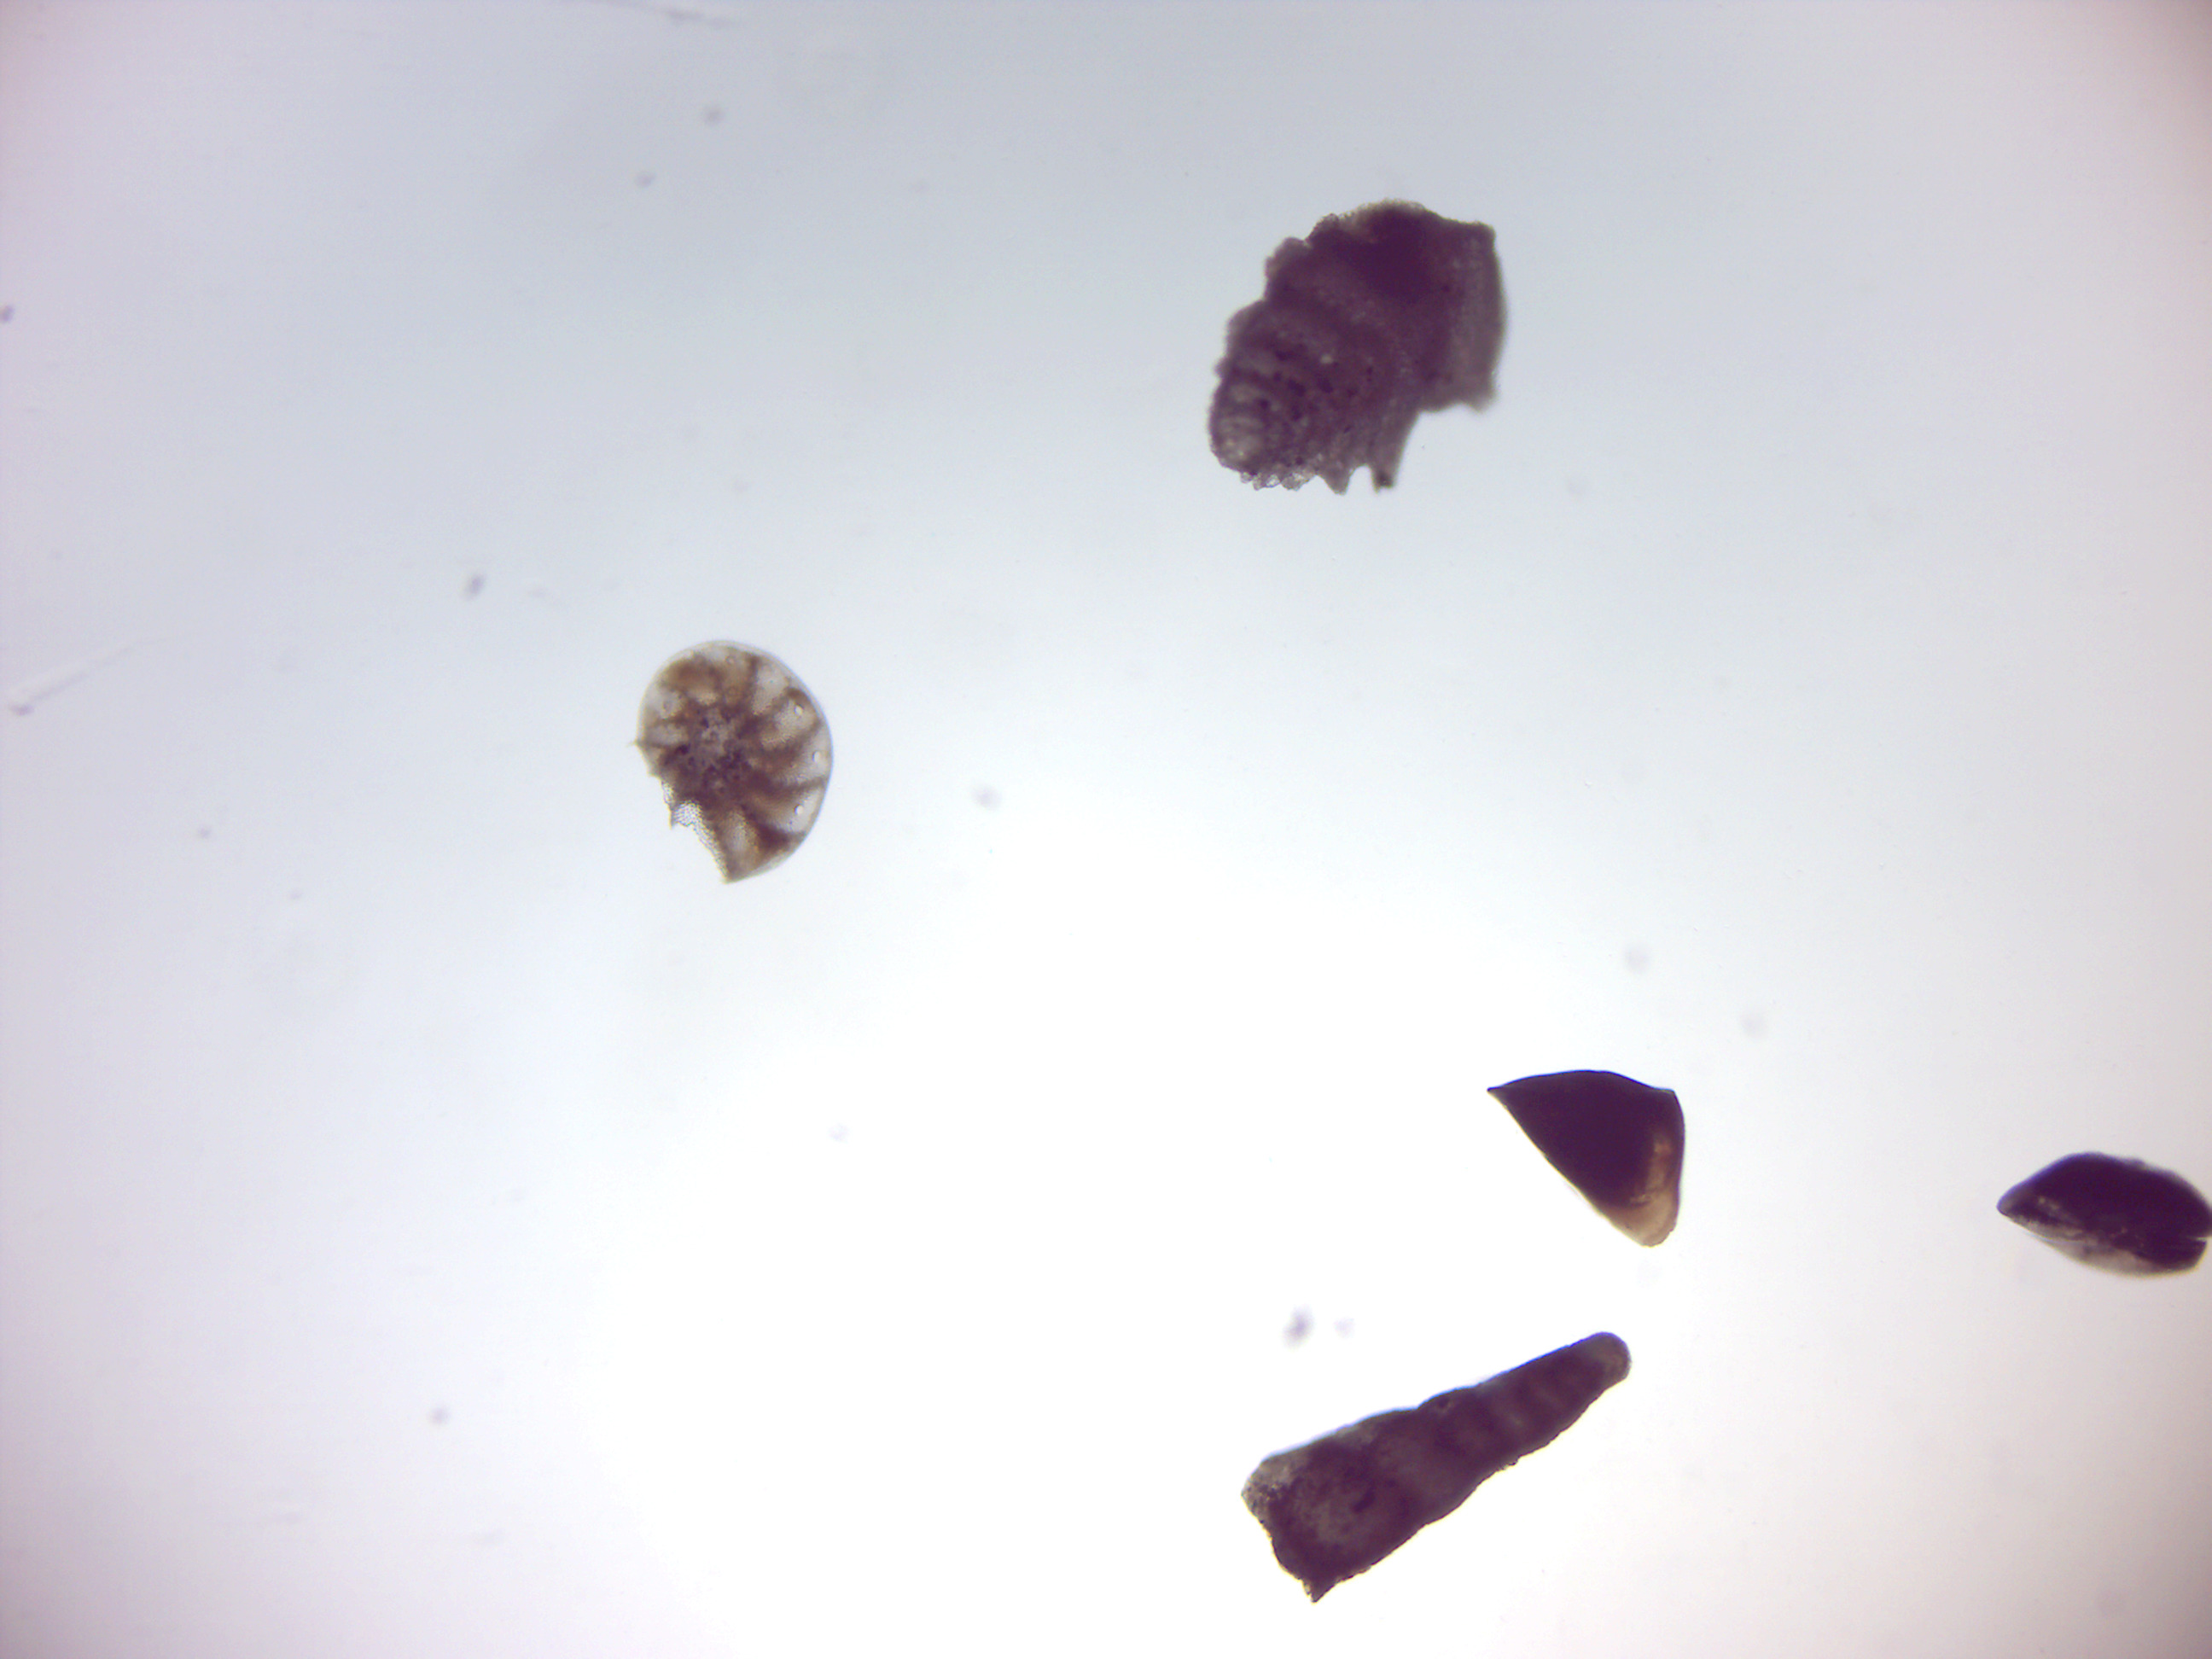
\includegraphics[width=0.7\linewidth]{./figures/protists/foraminifera} 

}

\caption{Foraminifera.}\label{fig:foraminifera}
\end{figure}

\subsection{Radiolaria}\label{radiolaria}

\href{https://en.wikipedia.org/wiki/Radiolaria}{\emph{Radiolaria}}
(Figure \ref{fig:radiolaria}), also called Radiozoa, are protozoa of
diameter 0.1-0.2 mm that produce intricate mineral skeletons, typically
with a central capsule dividing the cell into the inner and outer
portions of endoplasm and ectoplasm.The elaborate mineral skeleton is
usually made of silica. They are found as zooplankton throughout the
ocean, and their skeletal remains make up a large part of the cover of
the ocean floor as siliceous ooze.

\begin{figure}

{\centering 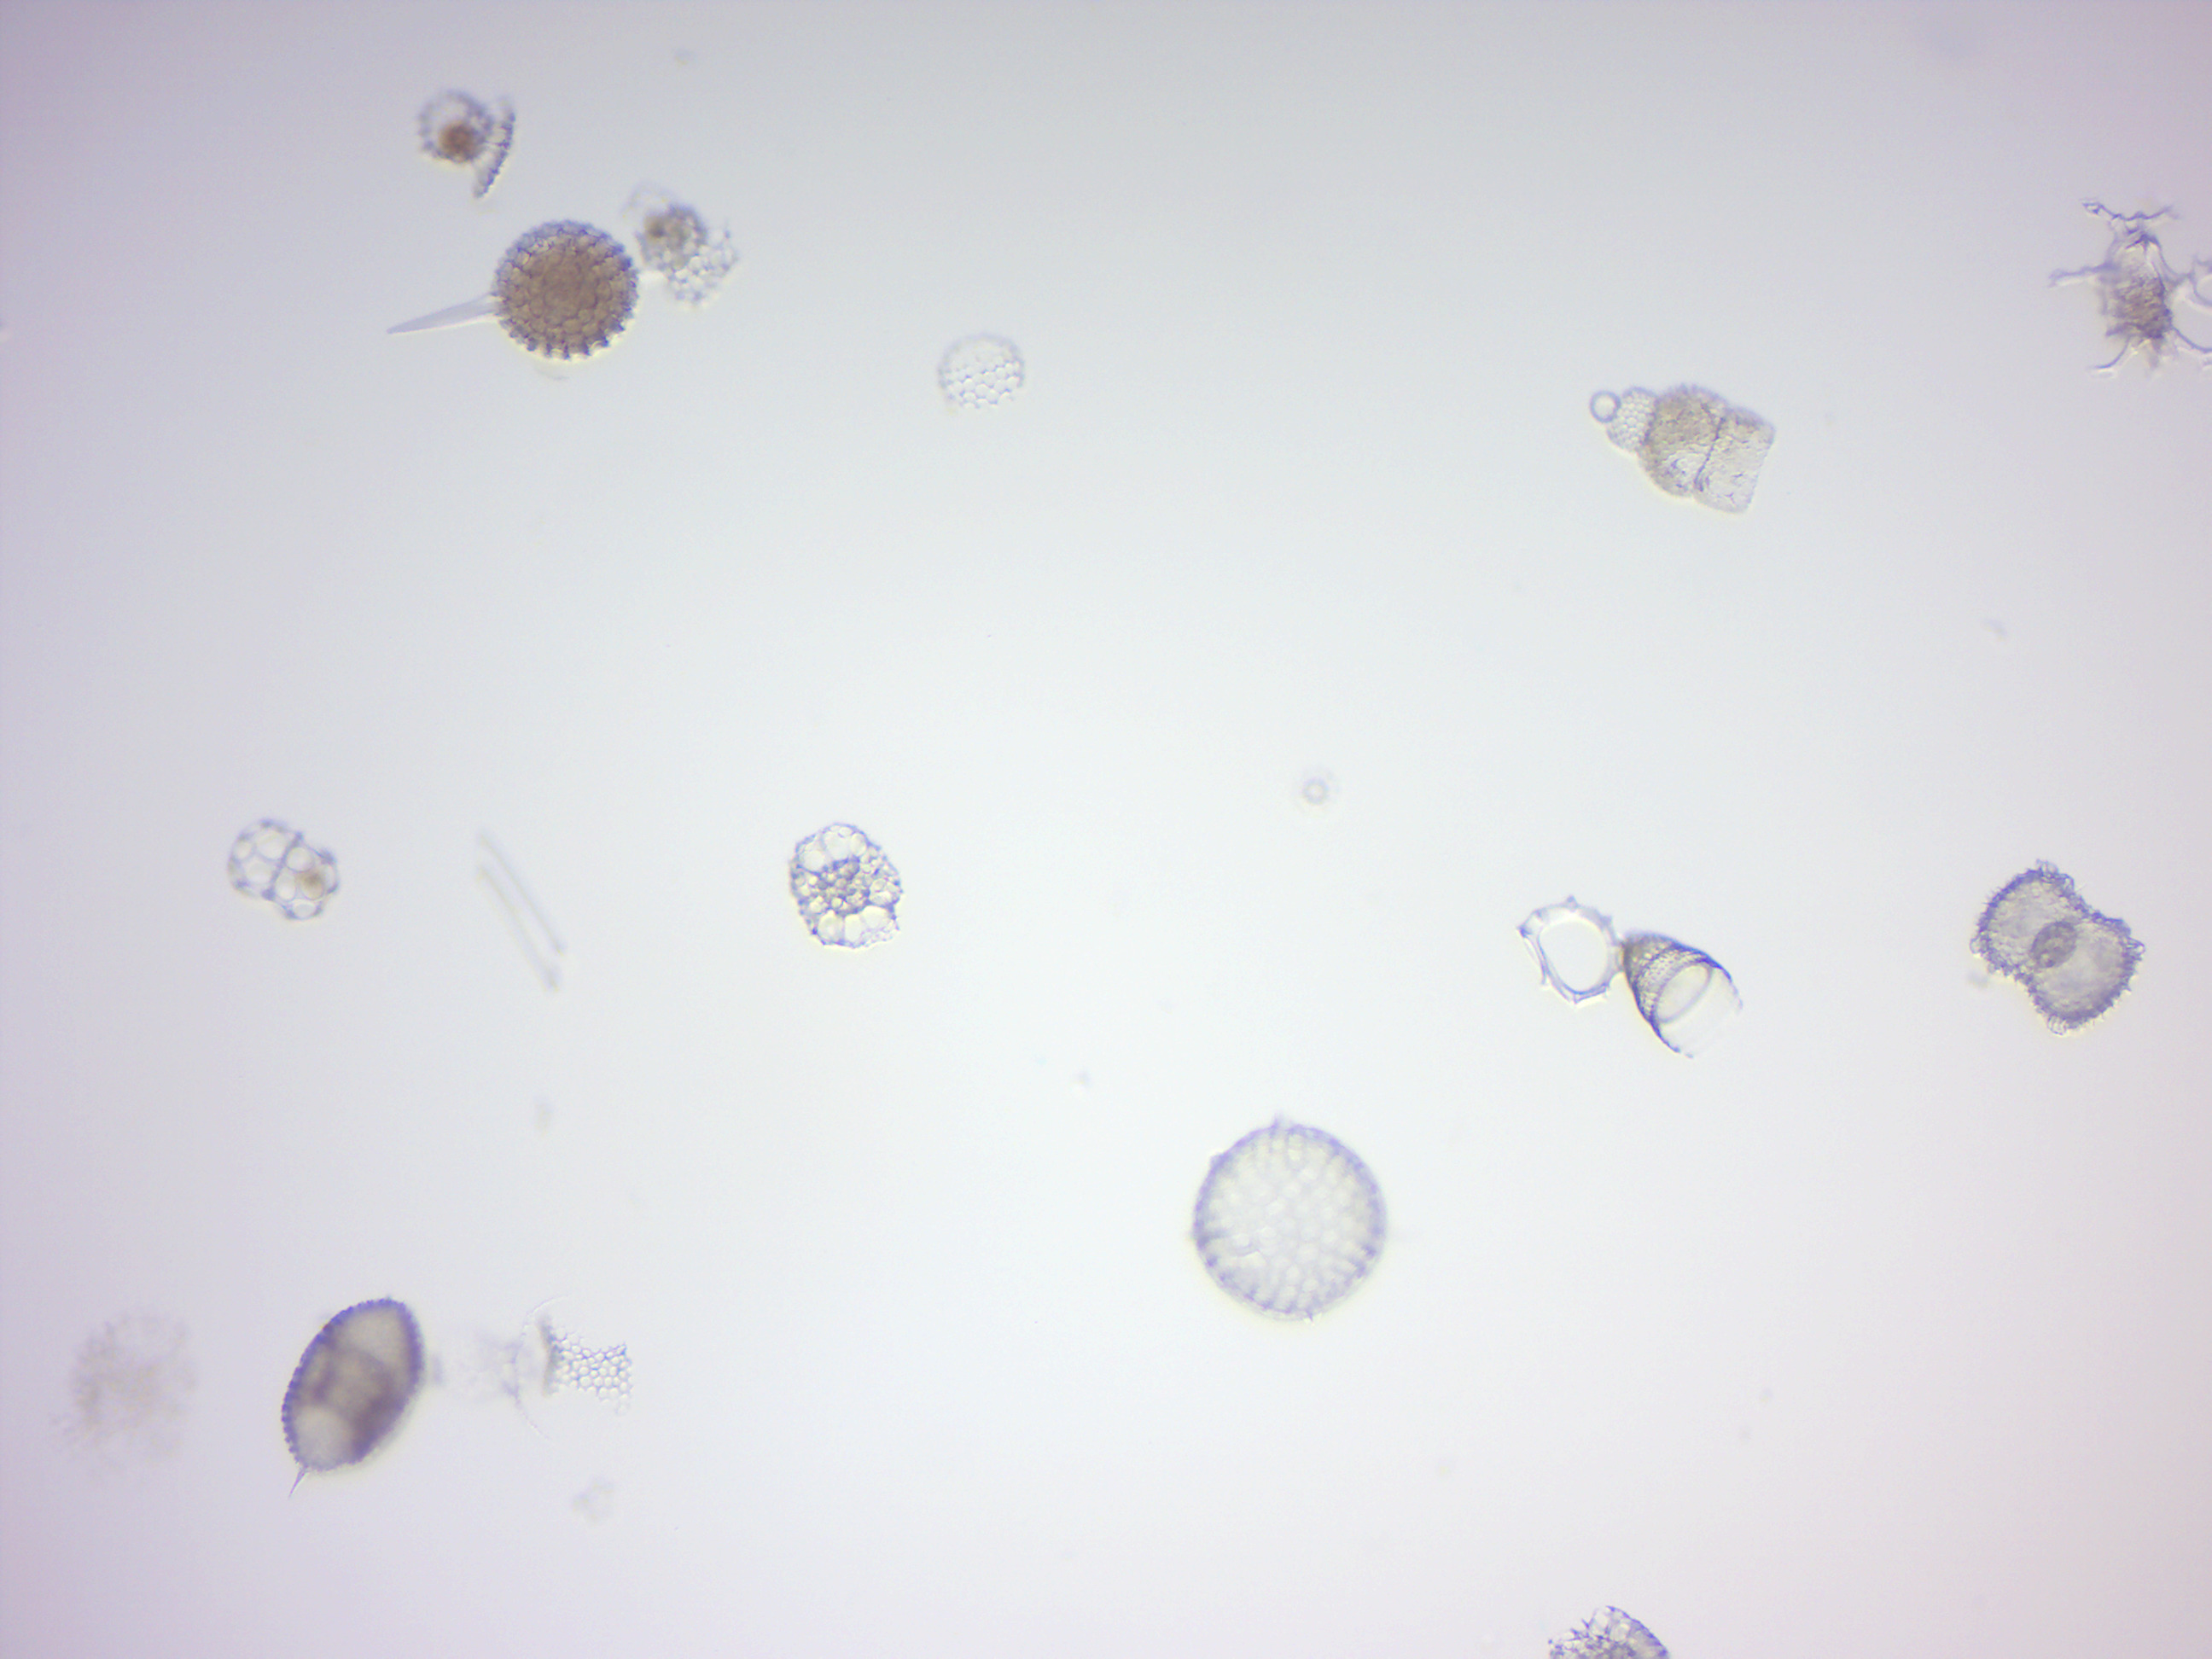
\includegraphics[width=0.7\linewidth]{./figures/protists/radiolaria} 

}

\caption{Radiolaria.}\label{fig:radiolaria}
\end{figure}

\subsection{Diatoms}\label{diatoms}

\href{https://en.wikipedia.org/wiki/Diatom}{\emph{Diatoms}} (Figure
\ref{fig:diatomes}) are a major group of microalgae and are among the
most common types of phytoplankton. Diatoms are producers within the
food chain. A unique feature of diatom cells is that they are enclosed
within a cell wall made of silica (hydrated silicon dioxide) called a
frustule. These frustules show a wide diversity in form, but are usually
almost bilaterally symmetrical, hence the group name. These shells are
used by humans as diatomaceous earth, also known as diatomite. Fossil
evidence suggests that they originated during, or before, the early
Jurassic period. Only male gametes of centric diatoms are capable of
movement by means of flagella. Diatom communities are a popular tool for
monitoring environmental conditions, past and present, and are commonly
used in studies of water quality.

\begin{figure}

{\centering 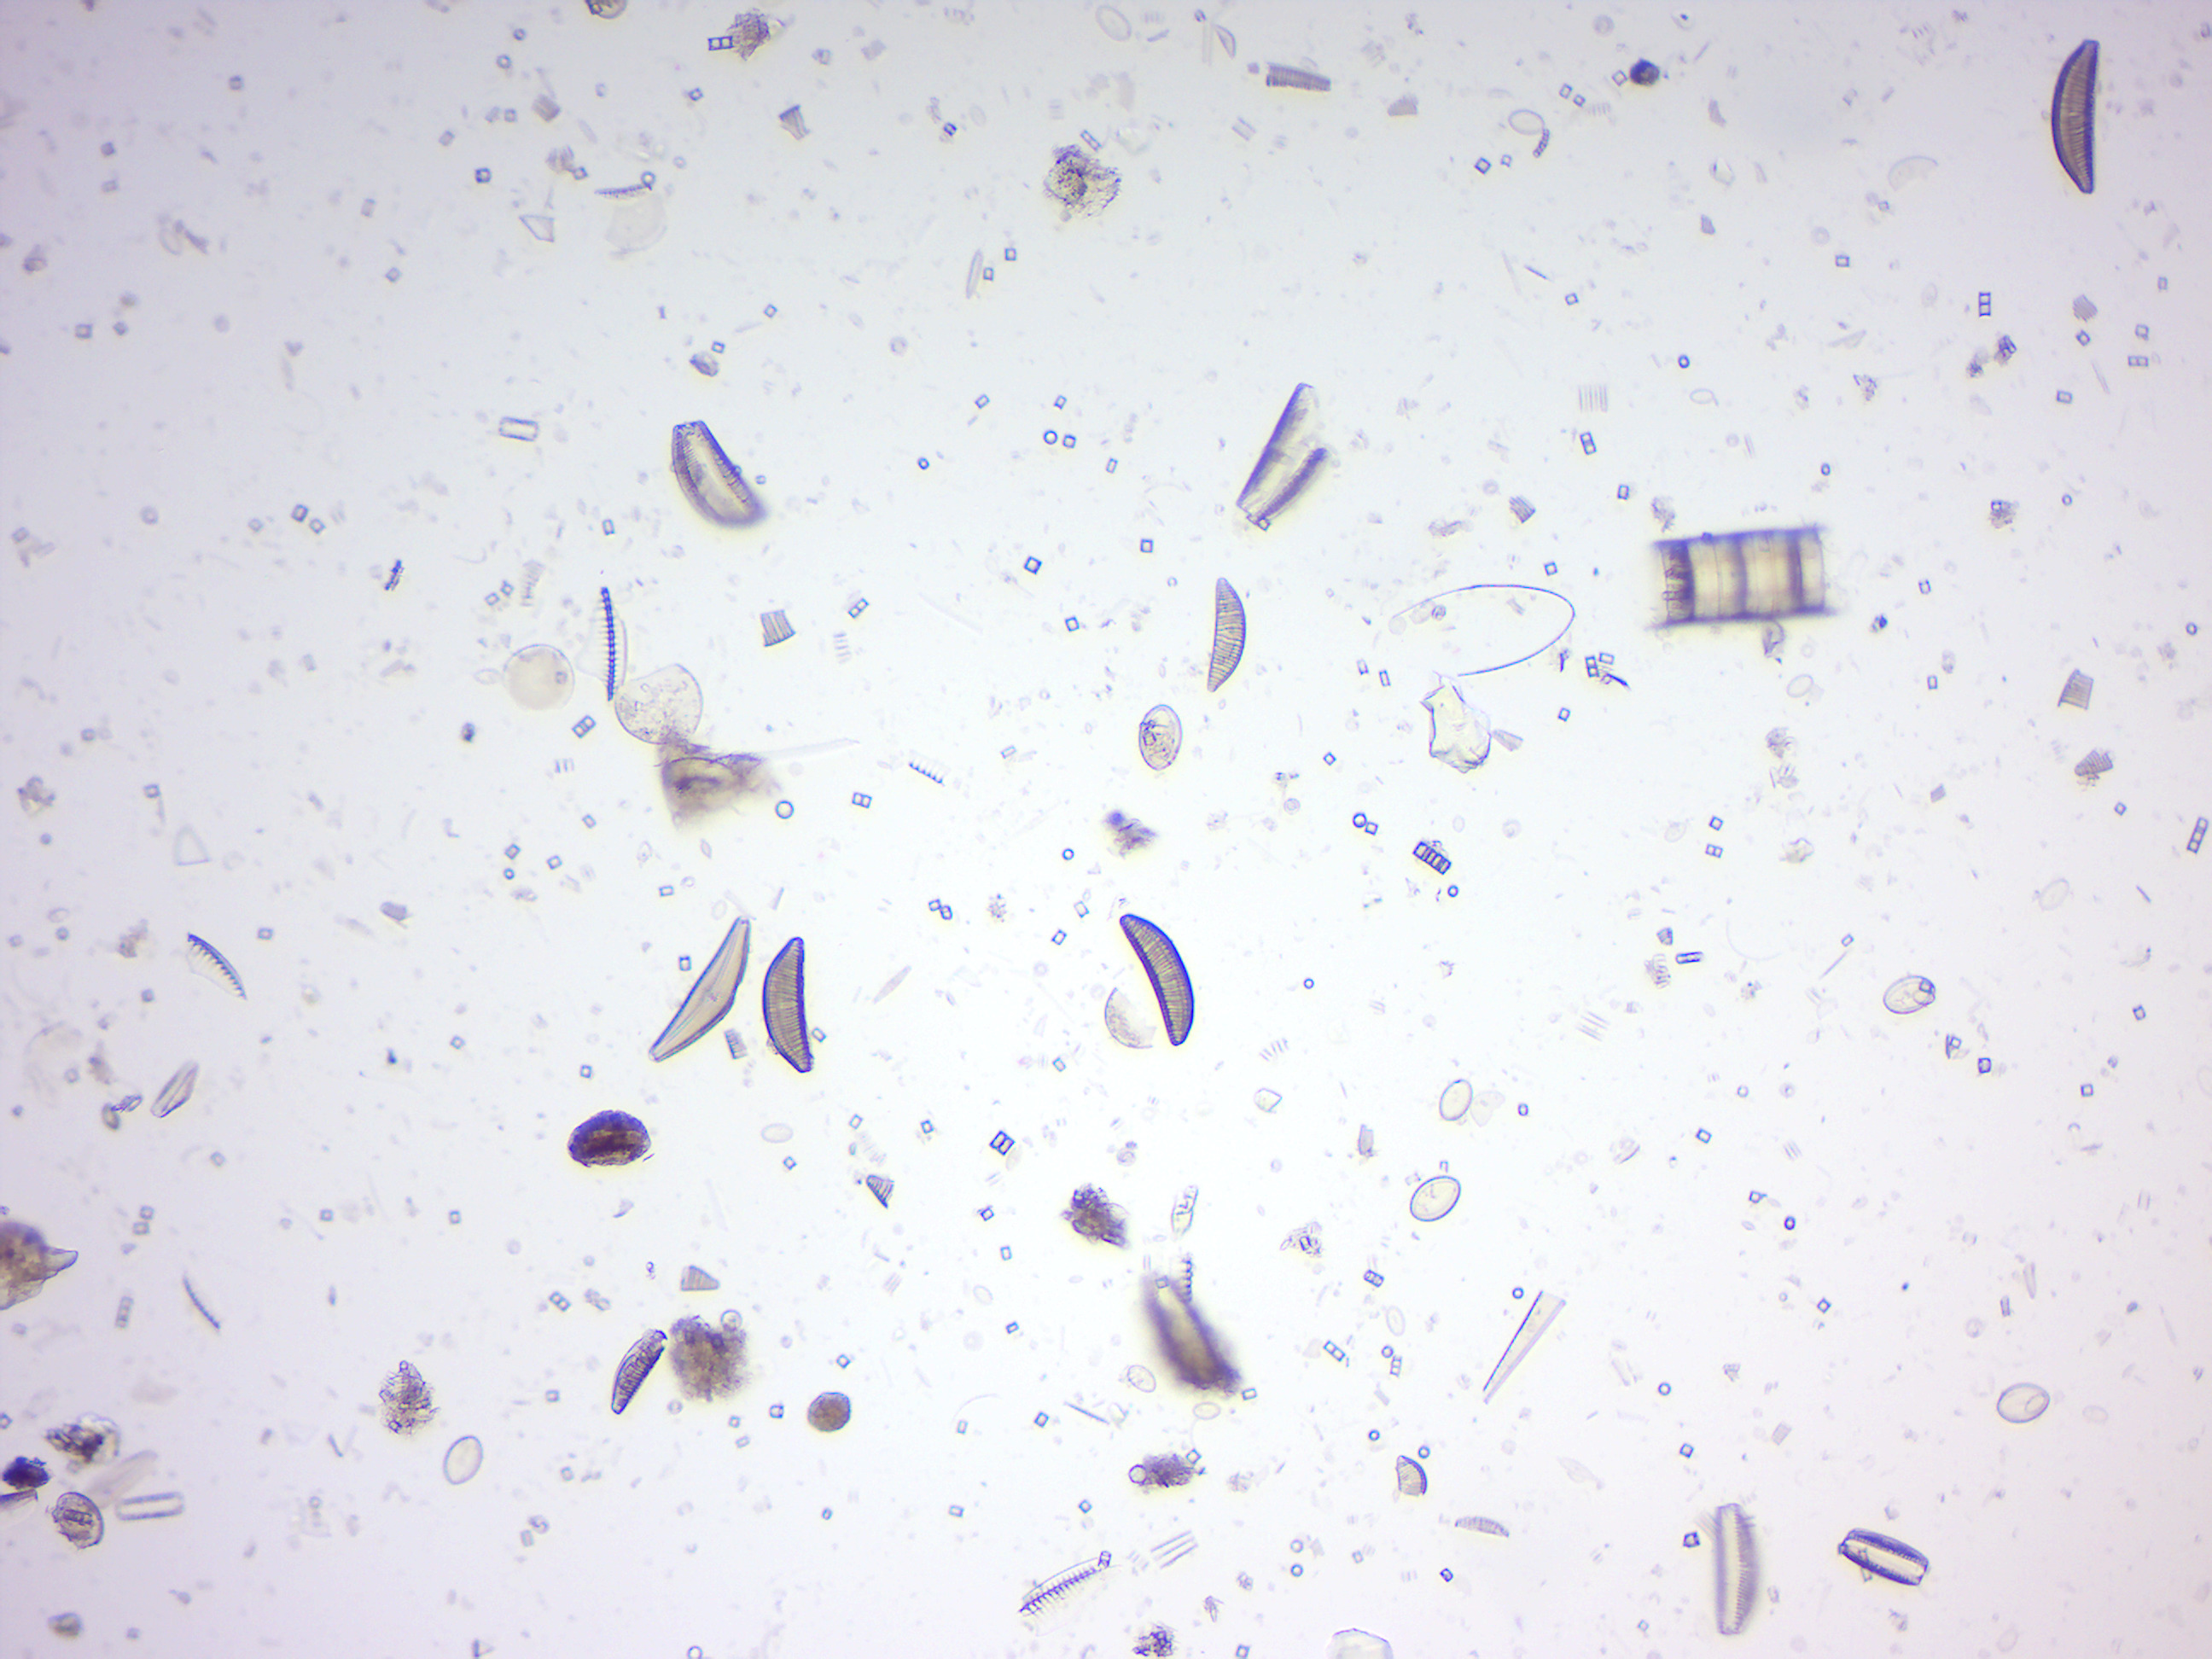
\includegraphics[width=0.7\linewidth]{./figures/protists/diatomes} 

}

\caption{Diatomes.}\label{fig:diatomes}
\end{figure}

\subsection{\texorpdfstring{\emph{Trypanosoma cruzi} and
\emph{Trypanosoma brucei
gambiense}}{Trypanosoma cruzi and Trypanosoma brucei gambiense}}\label{trypanosoma-cruzi-and-trypanosoma-brucei-gambiense}

\href{https://en.wikipedia.org/wiki/Trypanosoma_cruzi}{\emph{Trypanosoma
cruzi}} is a species of parasitic euglenoids. Amongst the protozoa, the
trypanosomes characteristically bore tissue in another organism and feed
on blood (primarily) and also lymph. This behaviour causes disease or
the likelihood of disease that varies with the organism: for example,
trypanosomiasis in humans (Chagas disease in South America). Parasites
need a host body and the haematophagous insect triatomine (descriptions
``assassin bug'', ``cone-nose bug'', and ``kissing bug'') is the major
vector in accord with a mechanism of infection. The triatomine likes the
nests of vertebrate animals for shelter, where it bites and sucks blood
for food. Individual triatomines infected with protozoa from other
contact with animals transmit trypanosomes when the triatomine deposits
its faeces on the host's skin surface and then bites. Penetration of the
infected faeces is further facilitated by the scratching of the bite
area by the human or animal host.

\href{https://en.wikipedia.org/wiki/Trypanosoma_brucei}{\emph{Trypanosoma
brucei}} (Figure \ref{fig:gambiense}) is a species of parasitic
kinetoplastid belonging to the genus Trypanosoma. The parasite is the
cause of a vector-borne disease of vertebrate animals, including humans,
carried by genera of tsetse fly in sub-Saharan Africa. In humans
\emph{T. brucei} causes African trypanosomiasis, or sleeping sickness.
In animals it causes animal trypanosomiasis, also called nagana in
cattle and horses. \emph{T. brucei} has traditionally been grouped into
three subspecies: \emph{T. b. brucei}, \emph{T. b. gambiense} and
\emph{T. b. rhodesiense}. The first is a parasite of non-human
vertebrates, while the latter two are the known parasites of humans.

\begin{figure}

{\centering 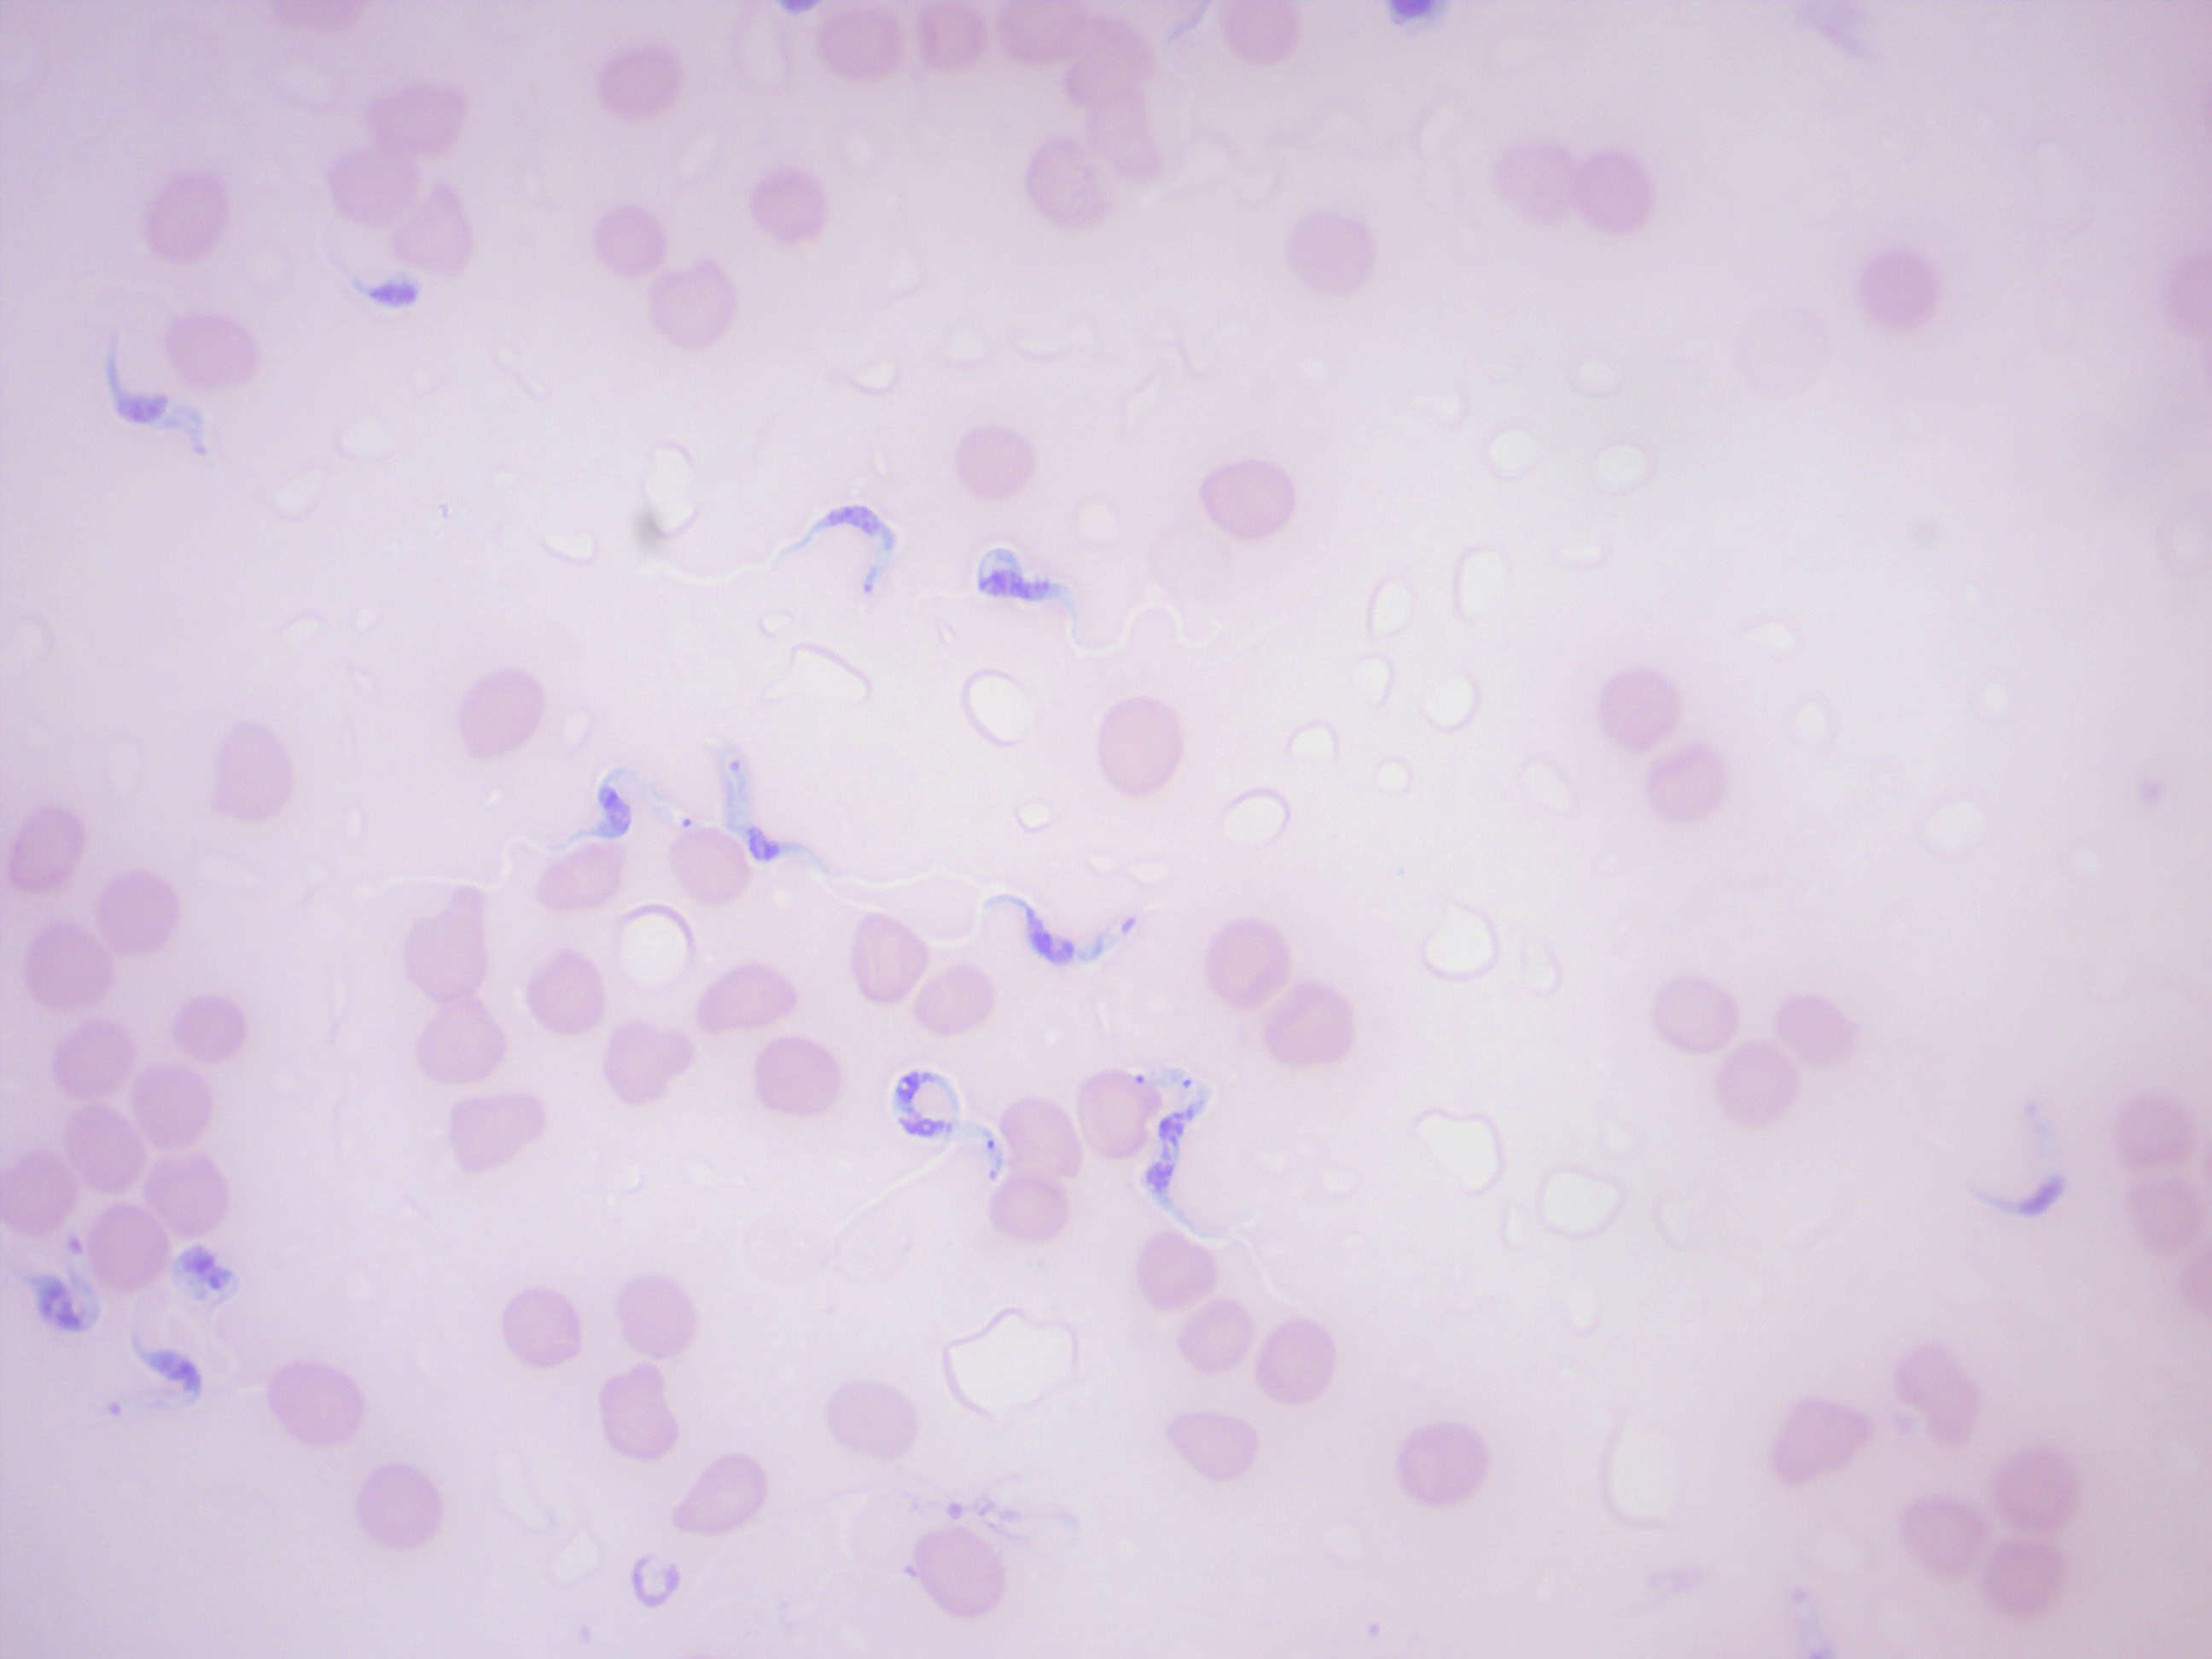
\includegraphics[width=0.7\linewidth]{./figures/protists/gambiense} 

}

\caption{Trypanosoma brucei gambiense among red blood cells.}\label{fig:gambiense}
\end{figure}

\subsection{Plasmodium vivax}\label{plasmodium-vivax}

\href{https://en.wikipedia.org/wiki/Plasmodium_vivax}{\emph{Plasmodium
vivax}} (Figure \ref{fig:plasmodium}) is a protozoal parasite and a
human pathogen. This parasite is the most frequent and widely
distributed cause of recurring (benign tertian) malaria, P. vivax is one
of the five species of malaria parasites that commonly infect humans.
Although it is less virulent than Plasmodium falciparum, the deadliest
of the five human malaria parasites, P. vivax malaria infections can
lead to severe disease and death, often due to a pathologically enlarged
spleen. P. vivax is carried by the female Anopheles mosquito, since it
is only the female of the species that bites.

\begin{figure}

{\centering 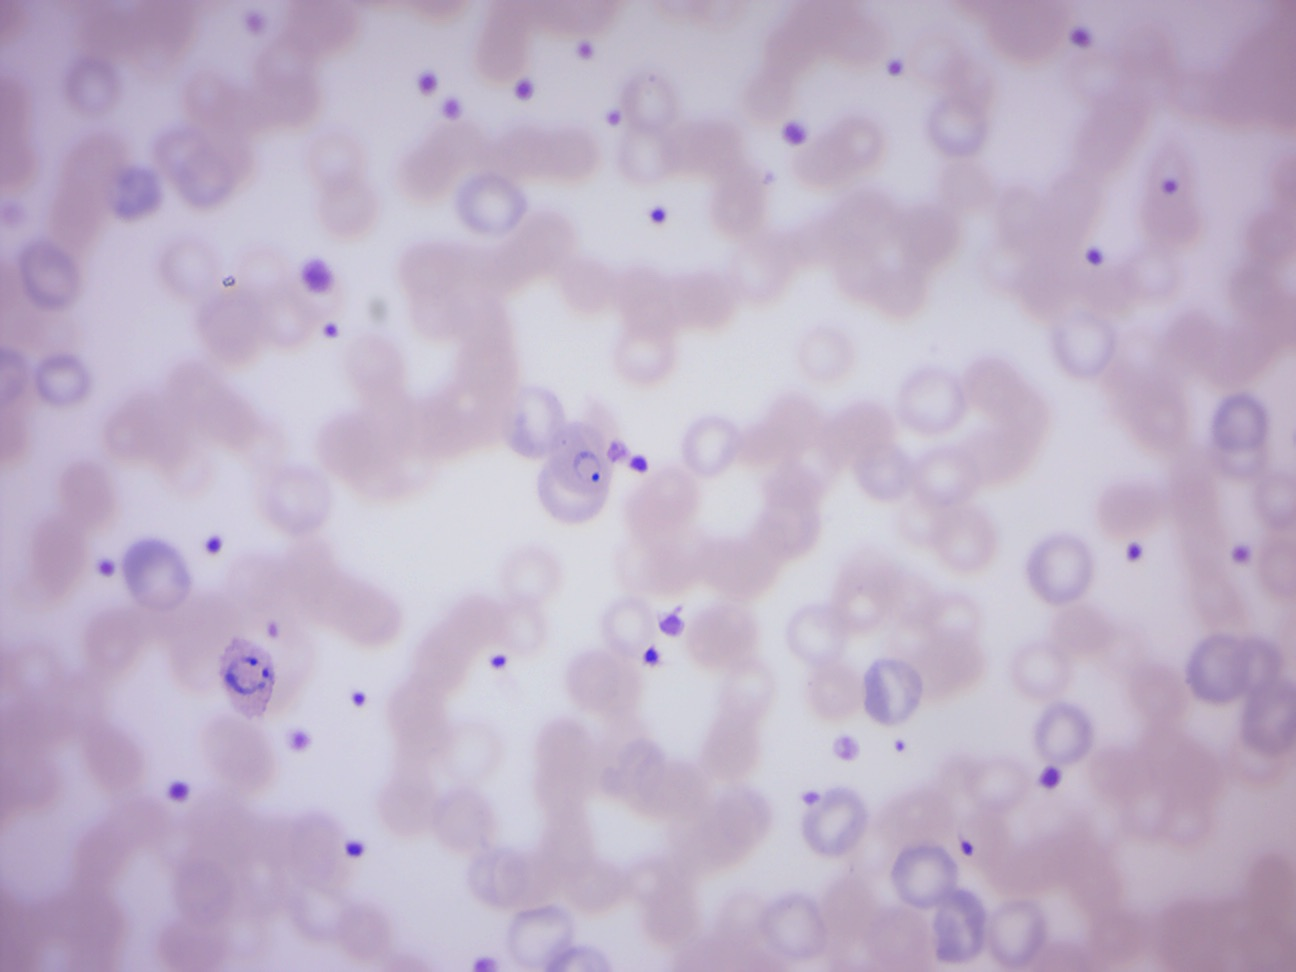
\includegraphics[width=0.7\linewidth]{./figures/protists/Plasmodium_vivax} 

}

\caption{Plasmodium vivax merozoites and trophozoites (ring stage).}\label{fig:plasmodium}
\end{figure}

\subsection{Mixed green algae (Figure
\ref{fig:mixedalgae})}\label{mixed-green-algae-figure-reffigmixedalgae}

\begin{figure}

{\centering 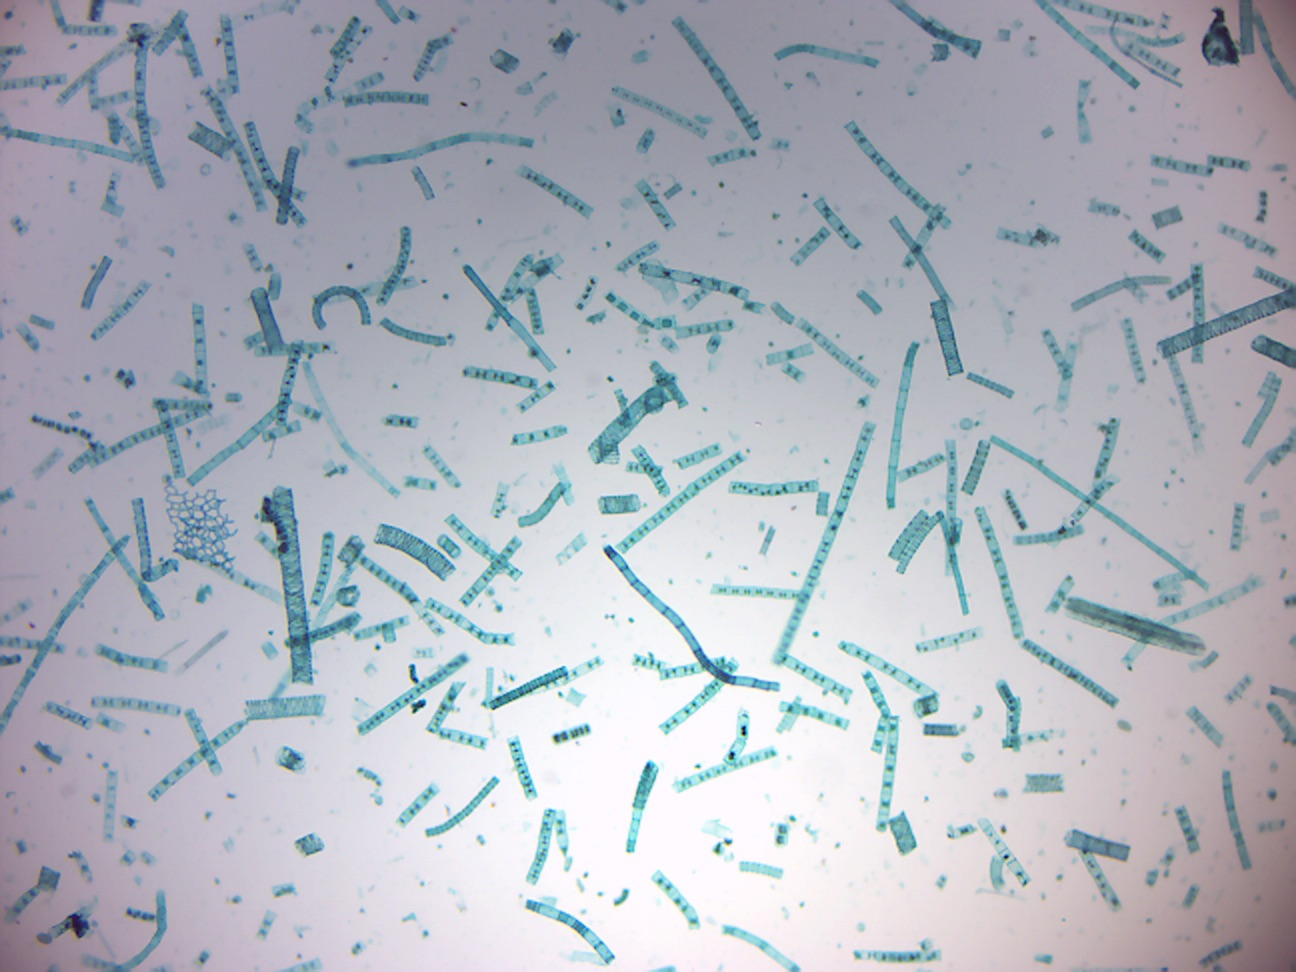
\includegraphics[width=0.7\linewidth]{./figures/protists/Mixed_green_algae} 

}

\caption{Various green algae.}\label{fig:mixedalgae}
\end{figure}

\subsection{Chlamydomonas (Figure
\ref{fig:chlamydomonas})}\label{chlamydomonas-figure-reffigchlamydomonas}

\begin{figure}

{\centering 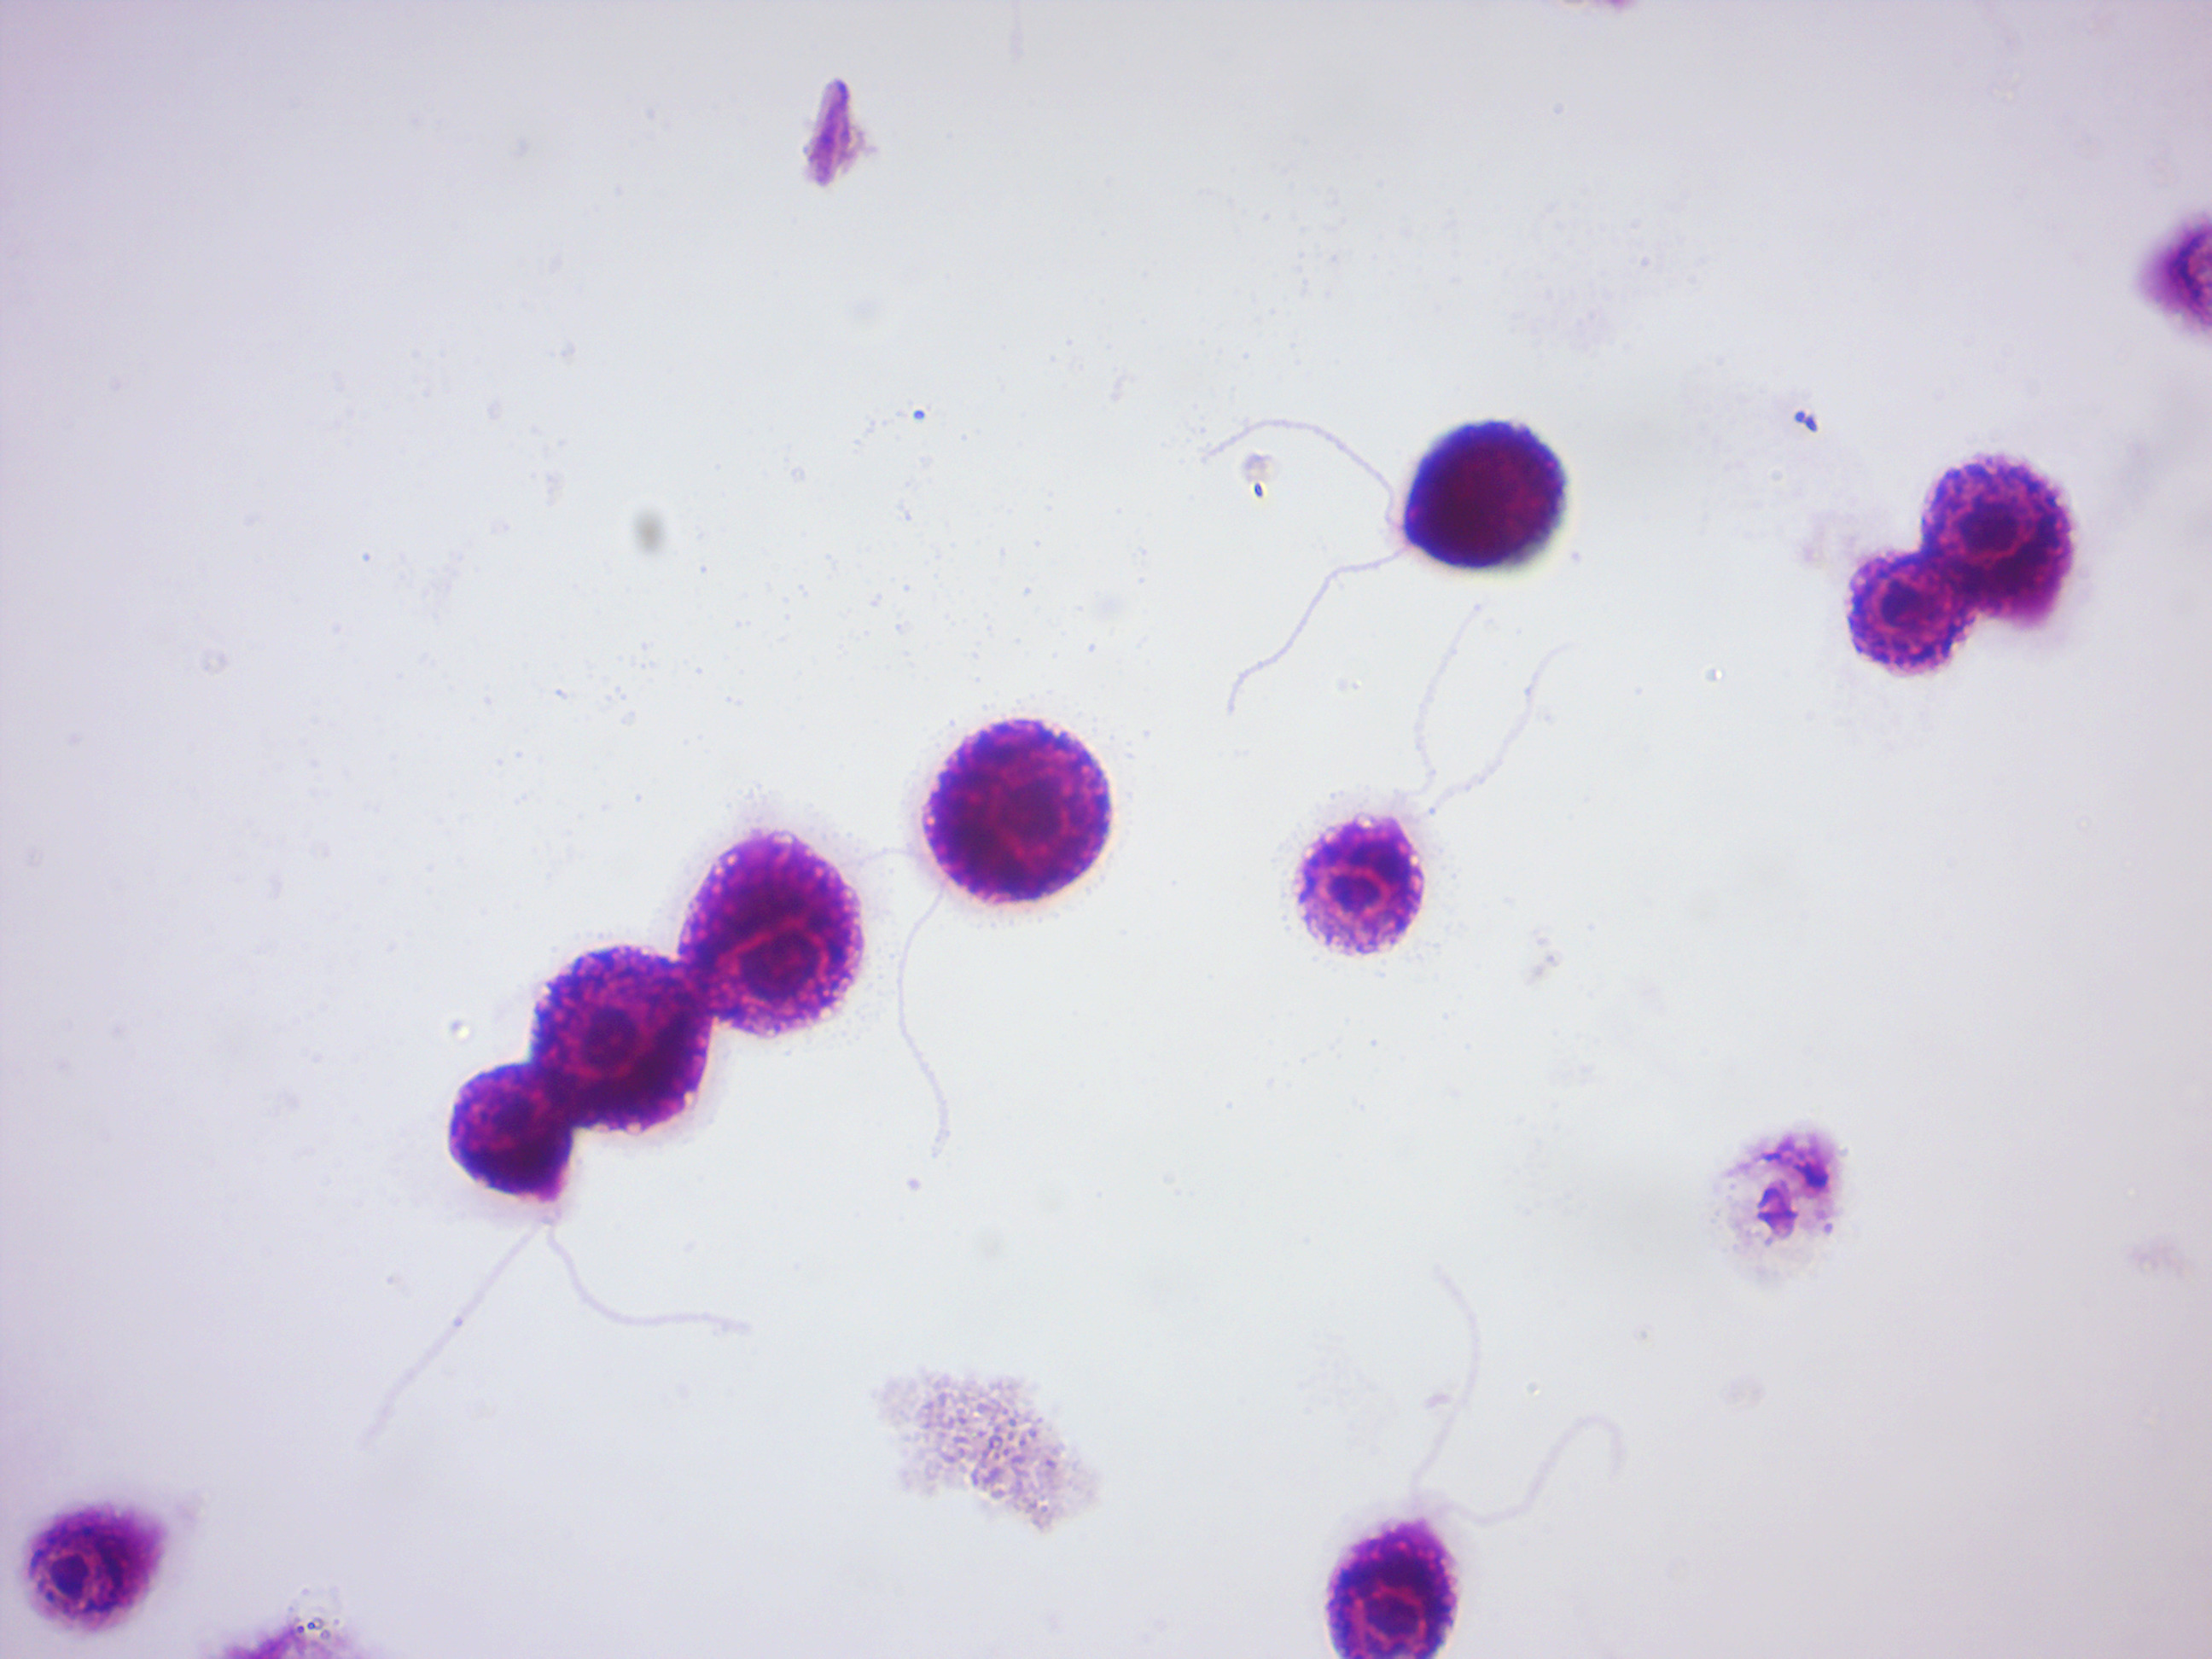
\includegraphics[width=0.7\linewidth]{./figures/protists/chlamydomonas} 

}

\caption{Chlamydomonas. Note the flagella.}\label{fig:chlamydomonas}
\end{figure}

\subsection{Pandorina (Figure
\ref{fig:pandorinadead})}\label{pandorina-figure-reffigpandorinadead}

\begin{figure}

{\centering 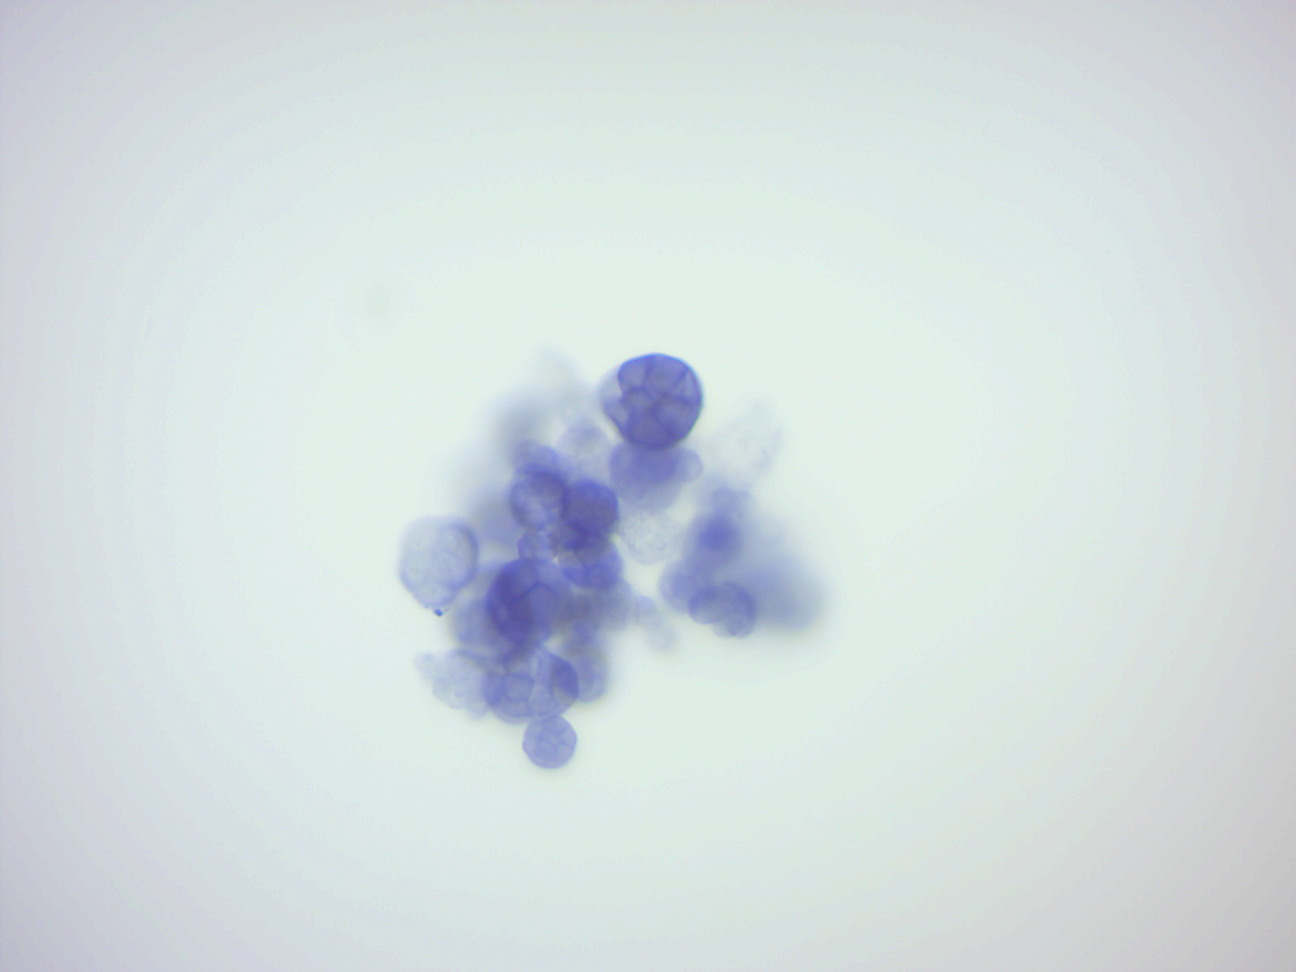
\includegraphics[width=0.7\linewidth]{./figures/protists/pandorinadead} 

}

\caption{Pandorina.}\label{fig:pandorinadead}
\end{figure}

\subsection{Volvox (Figure
\ref{fig:volvoxdead})}\label{volvox-figure-reffigvolvoxdead}

\begin{figure}

{\centering 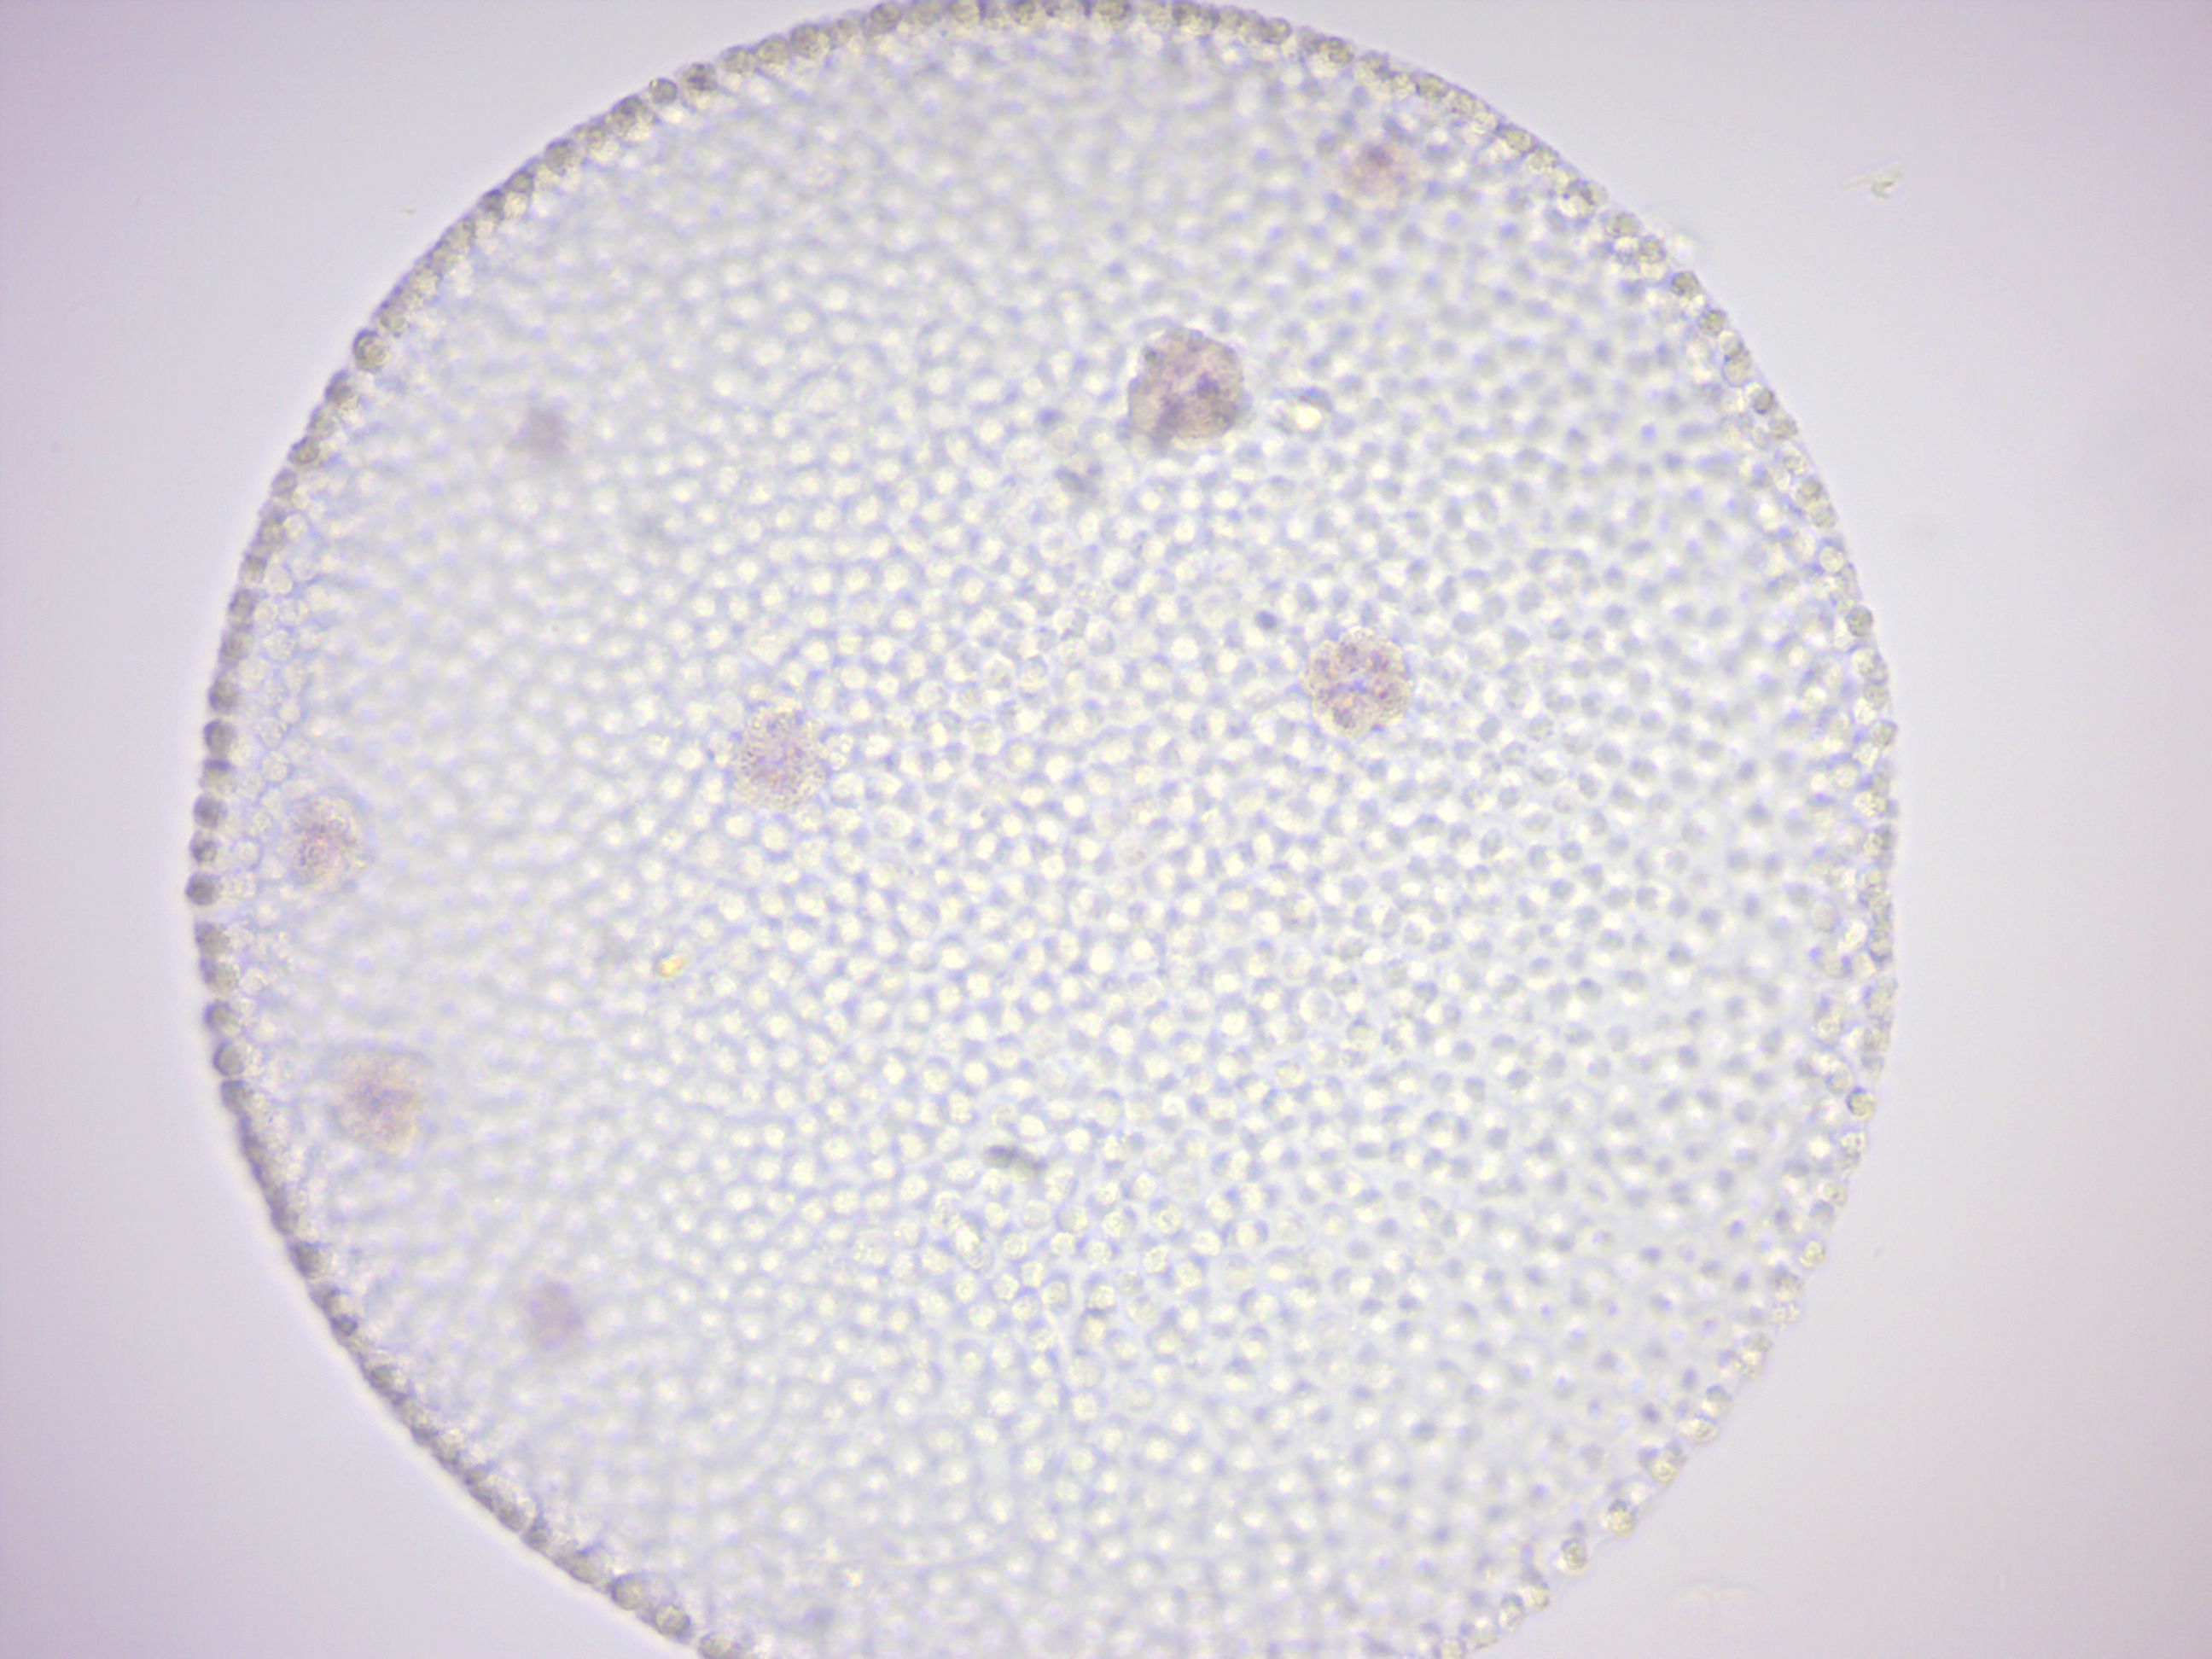
\includegraphics[width=0.7\linewidth]{./figures/protists/volvox_dead} 

}

\caption{Volvox.}\label{fig:volvoxdead}
\end{figure}

\subsection{Volvox sexual stages (Figure
\ref{fig:volvoxsex})}\label{volvox-sexual-stages-figure-reffigvolvoxsex}

\begin{figure}

{\centering 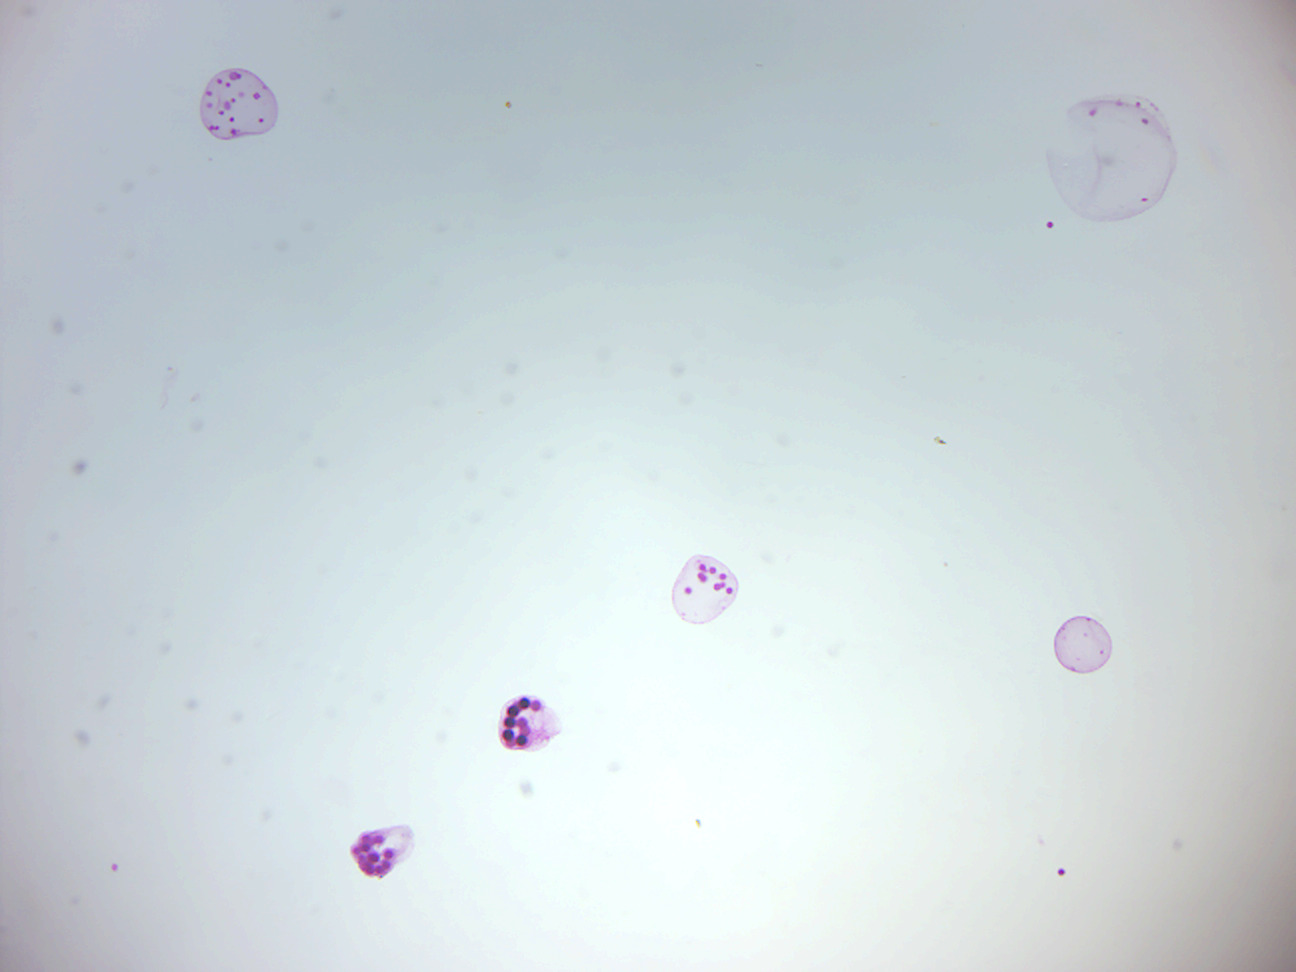
\includegraphics[width=0.7\linewidth]{./figures/protists/volvox_sex} 

}

\caption{Volvox sexual stages.}\label{fig:volvoxsex}
\end{figure}

\subsection{Spirogyra (Figure
\ref{fig:spirogyraprepared})}\label{spirogyra-figure-reffigspirogyraprepared}

\begin{figure}

{\centering 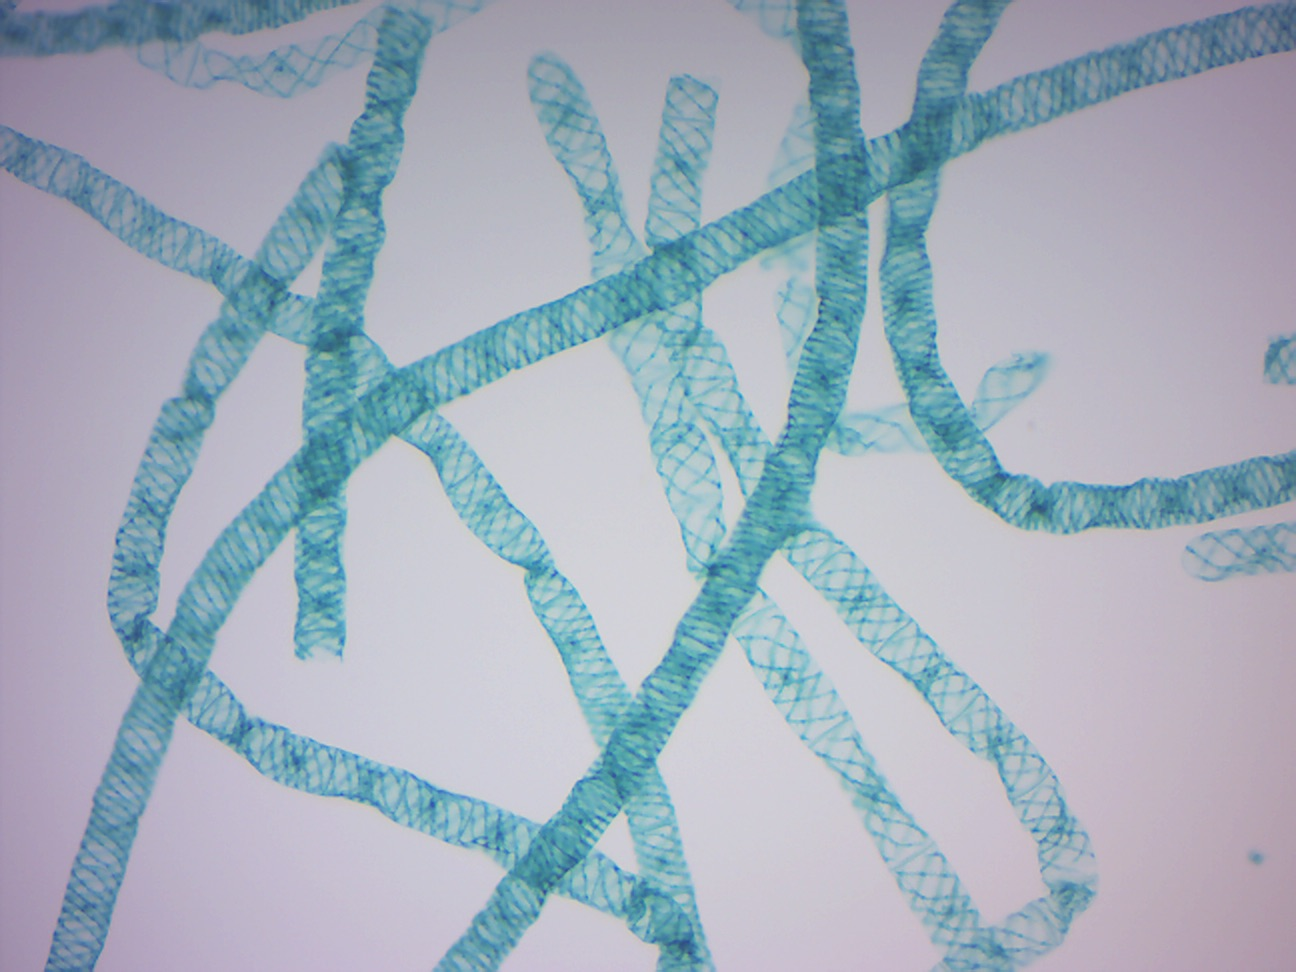
\includegraphics[width=0.7\linewidth]{./figures/protists/Spirogyra_prepared} 

}

\caption{Spirogyra.}\label{fig:spirogyraprepared}
\end{figure}

\subsection{Oedogonium zoospores (Figure
\ref{fig:oedogoniumzoospores}}\label{oedogonium-zoospores-figure-reffigoedogoniumzoospores}

\begin{figure}

{\centering 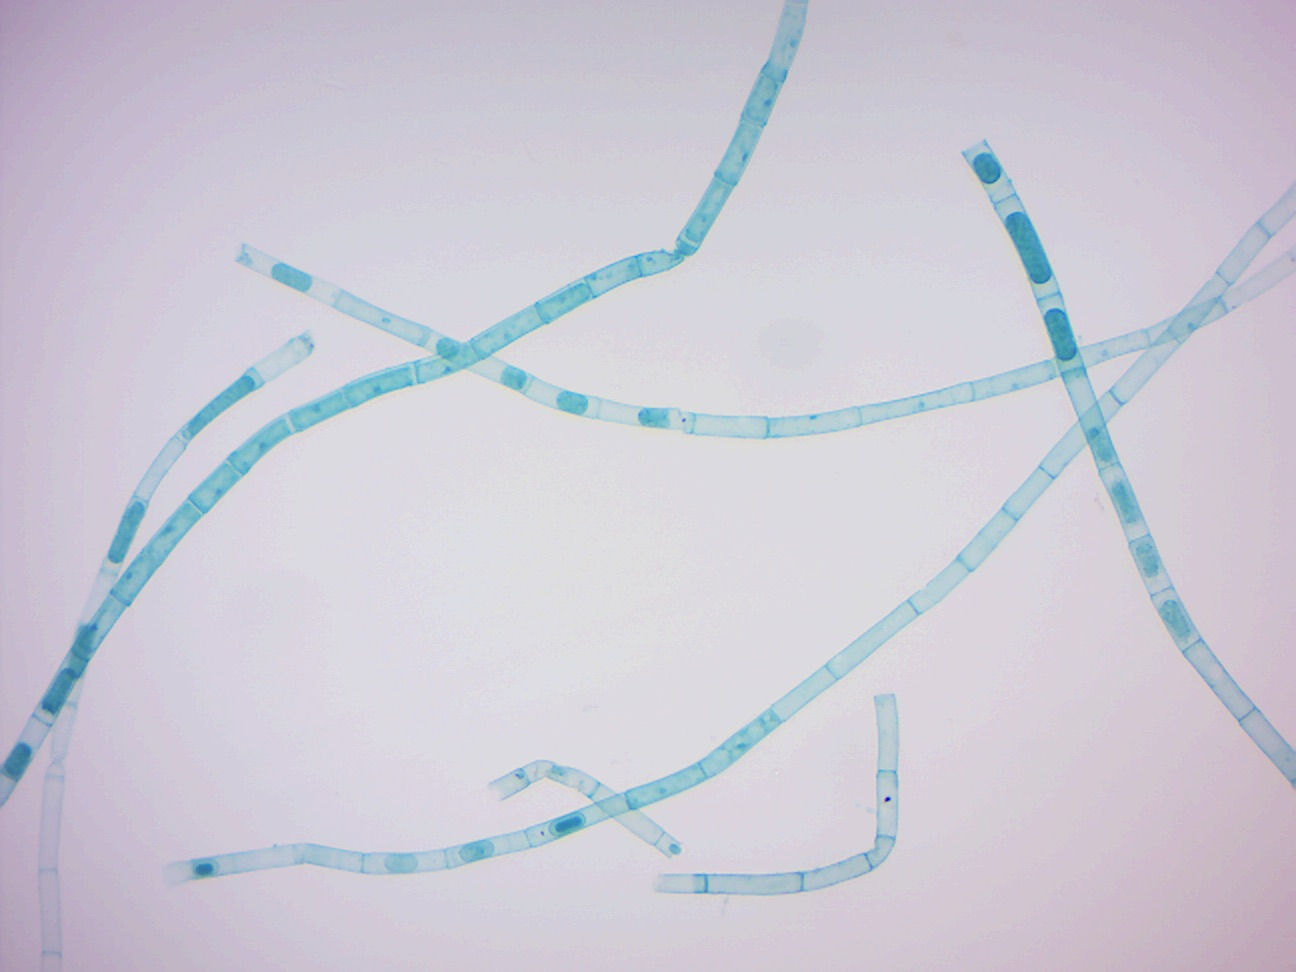
\includegraphics[width=0.7\linewidth]{./figures/protists/Oedogonium_zoospore_formation} 

}

\caption{Oedogonium zoospores.}\label{fig:oedogoniumzoospores}
\end{figure}

\subsection{Oedogonium macrandous (Figure
\ref{fig:oedogoniumprepared})}\label{oedogonium-macrandous-figure-reffigoedogoniumprepared}

\begin{figure}

{\centering 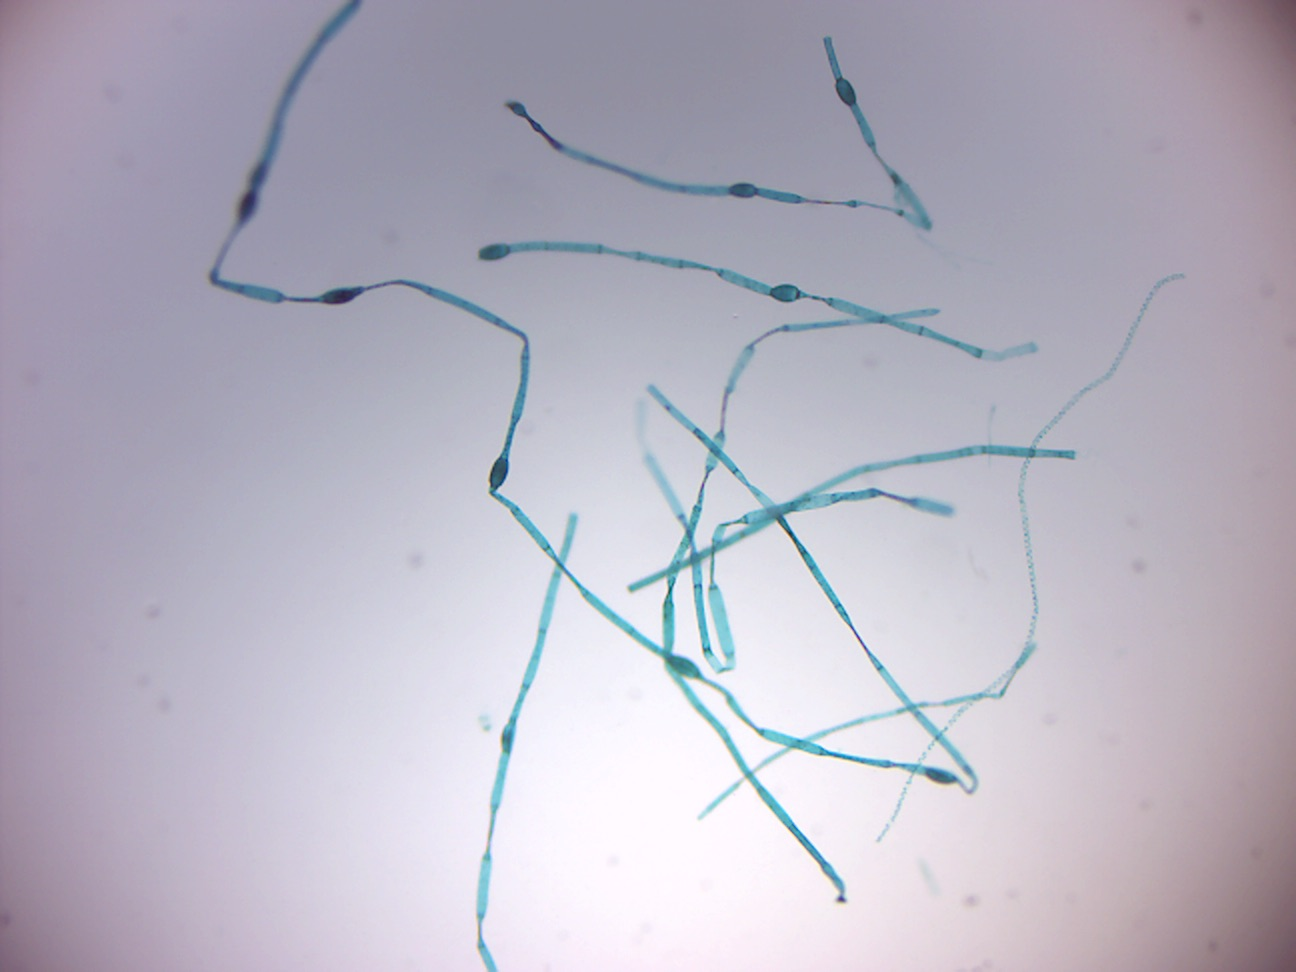
\includegraphics[width=0.7\linewidth]{./figures/protists/Oedogonium_macrandrous} 

}

\caption{Oedogonium.}\label{fig:oedogoniumprepared}
\end{figure}

\subsection{Fucus male and female
conceptacle}\label{fucus-male-and-female-conceptacle}

\href{https://en.wikipedia.org/wiki/Fucus}{\emph{Fucus}} is a genus of
brown algae found in the intertidal zones of rocky seashores almost
throughout the world. It has a relatively simple life cycle and produce
only one type of thallus which grows to a maximum size of 2 m. The
thallus is perennial with an irregular or disc-shaped holdfast or with
haptera. The erect portion of the thallus is dichotomous or subpinnately
branched, flattened and with a distinct midrib. Gas-filled pneumatocysts
(air-vesicles) are present in pairs in some species, one on either side
of the midrib. The gametangia develop in conceptacles embedded in
receptacles in the apices of the final branches. They may be monoecious
or dioecious. Fertile cavities, the conceptacles, containing the
reproductive cells are immersed in the receptacles near the ends of the
branches. After meiosis oogonia and antheridia are produced and
released, fertilisation follows and the zygote develops directly into
the diploid plant. It may be considered to be analogous to the life
cycle of the flowering plant, but in algae the oogonia are released and
fertilised in the sea while in flowering plants the ovules are
fertilised while attached to the parent plant and then released as a
seed.

\subsection{Fucus male conceptacle (Figure
\ref{fig:malefucus})}\label{fucus-male-conceptacle-figure-reffigmalefucus}

\begin{figure}

{\centering 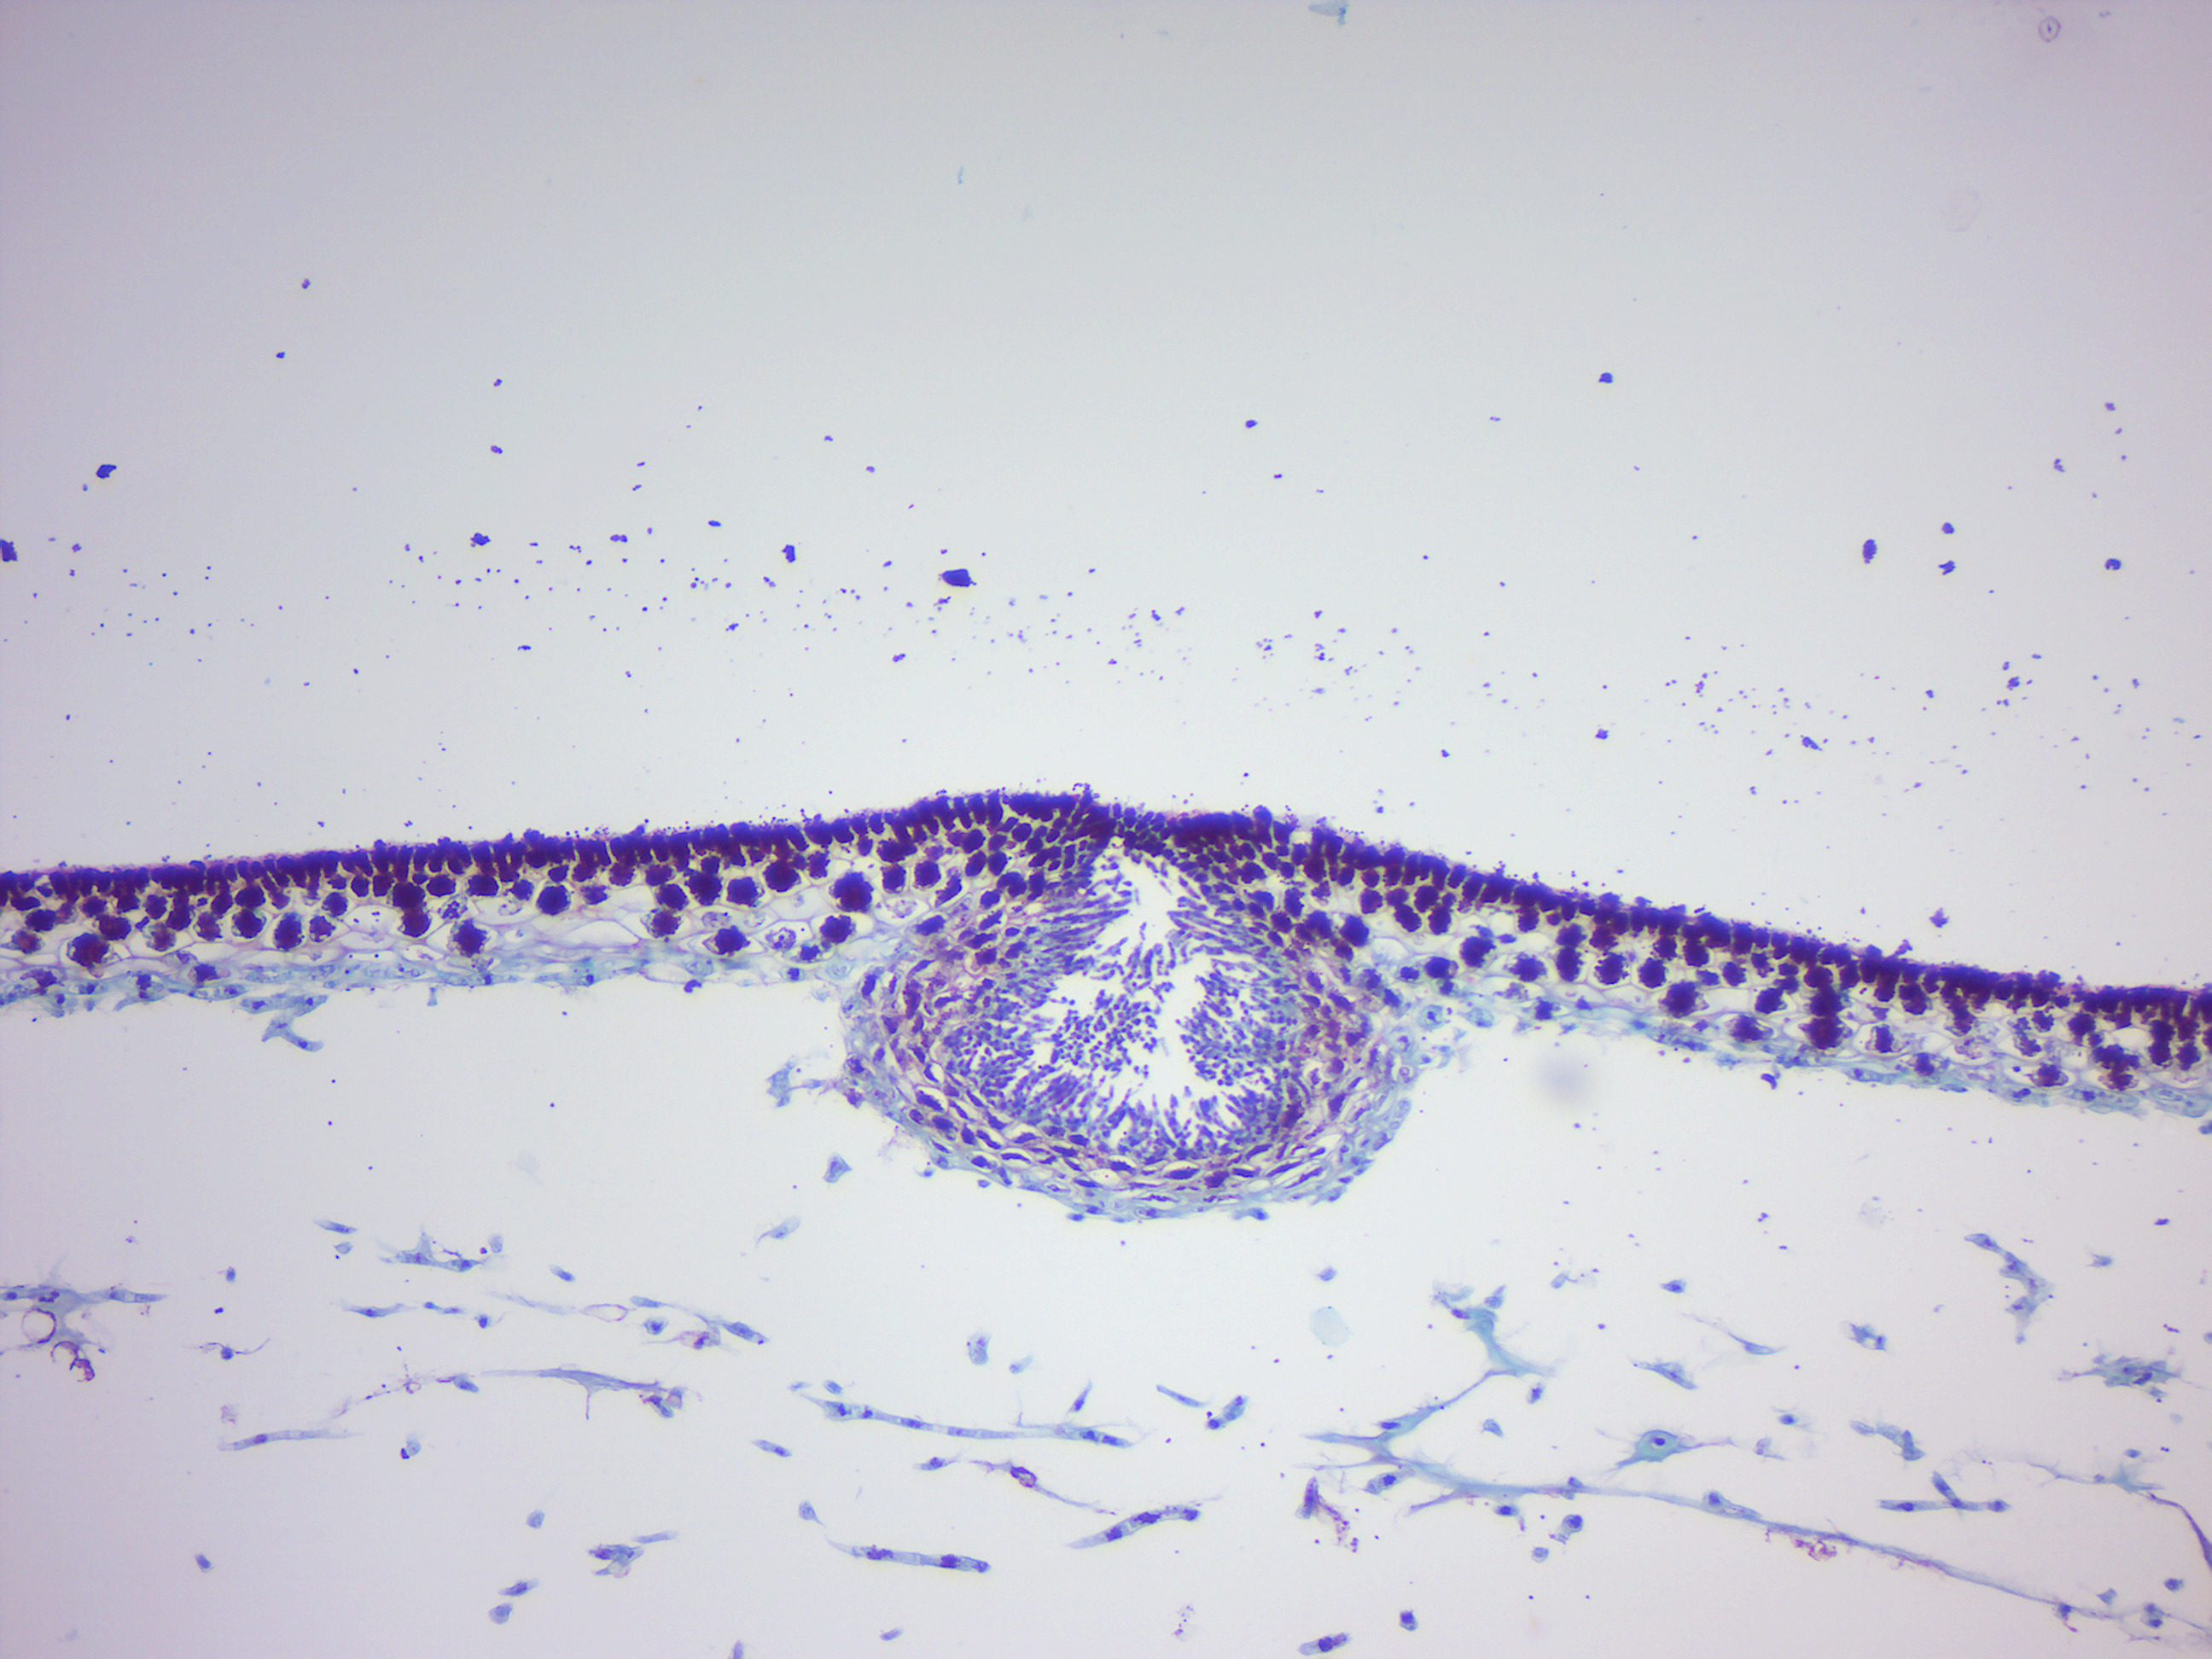
\includegraphics[width=0.7\linewidth]{./figures/protists/male_fucus} 

}

\caption{Fucus male conceptacle}\label{fig:malefucus}
\end{figure}

\subsection{Fucus female conceptacle (Figure
\ref{fig:femalefucus})}\label{fucus-female-conceptacle-figure-reffigfemalefucus}

\begin{figure}

{\centering 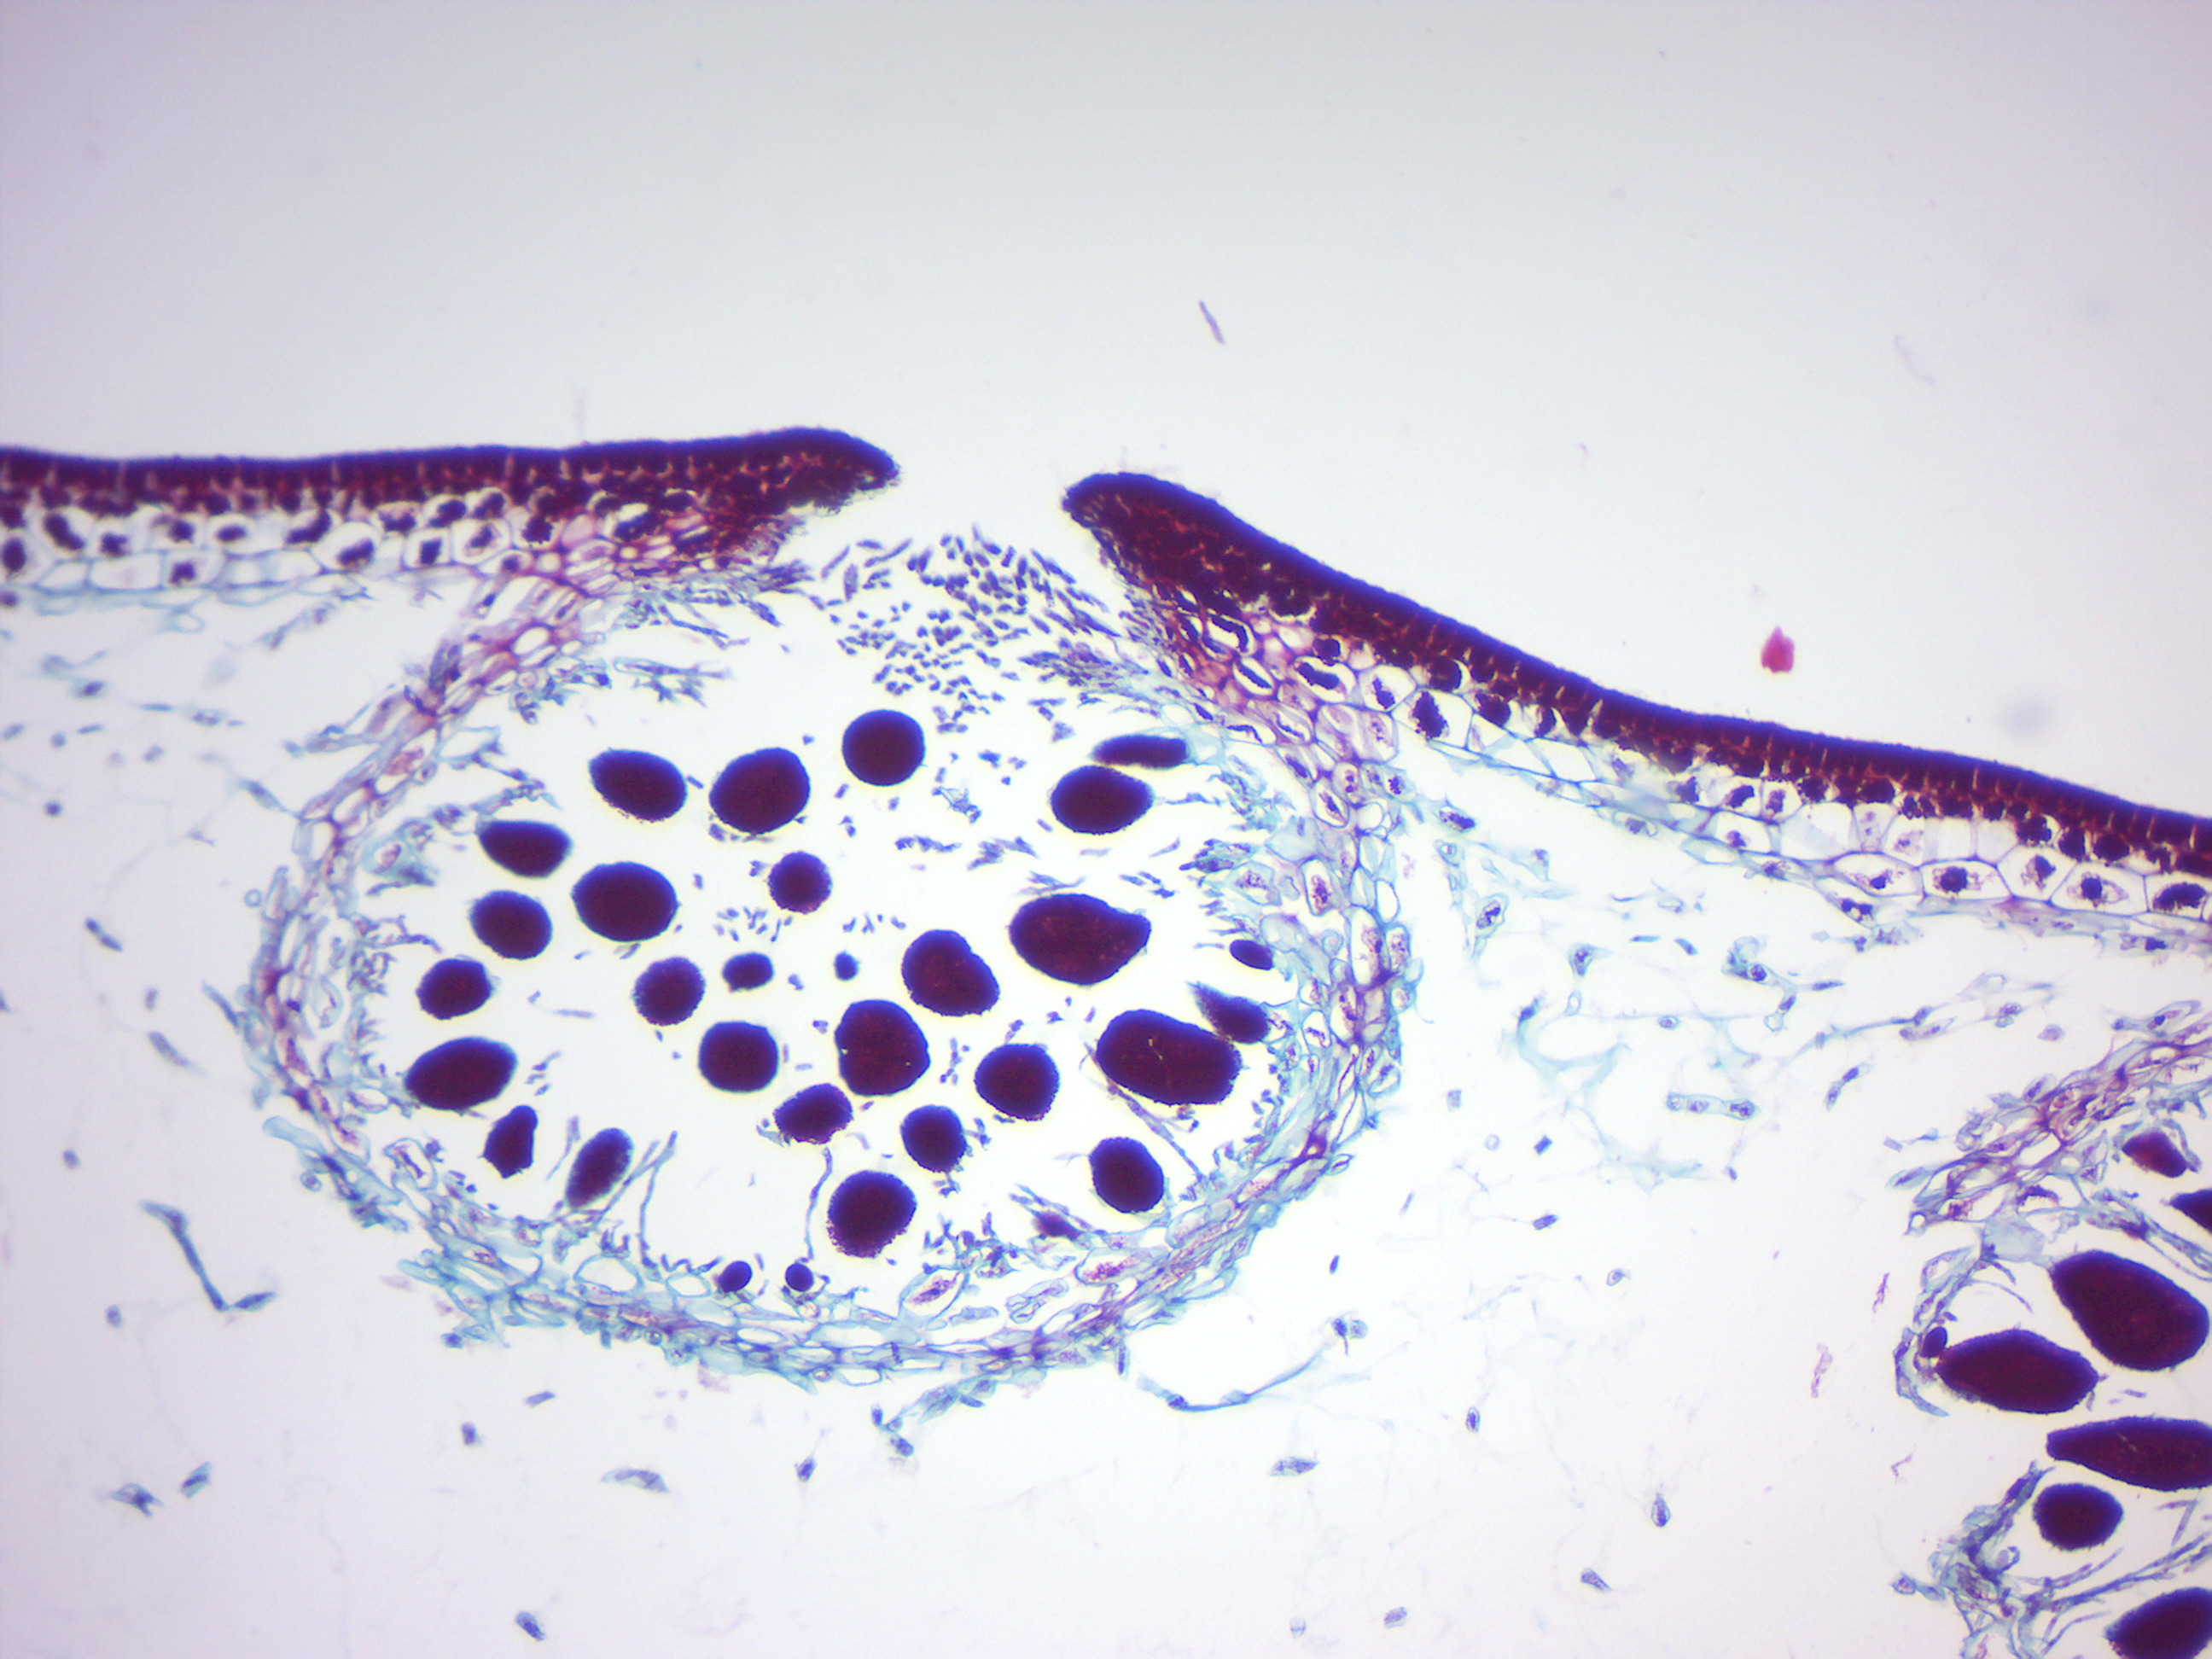
\includegraphics[width=0.7\linewidth]{./figures/protists/female_fucus} 

}

\caption{Fucus female conceptacle}\label{fig:femalefucus}
\end{figure}

\subsection{\texorpdfstring{\emph{Polysiphonia}}{Polysiphonia}}\label{polysiphonia}

\href{https://en.wikipedia.org/wiki/Polysiphonia}{\emph{Polysiphonia}}
(Figure \ref{fig:polysiphonia}) is a genus of filamentous red algae with
about 19 species on the coasts of the British Isles and about 200
species worldwide.

\begin{figure}

{\centering 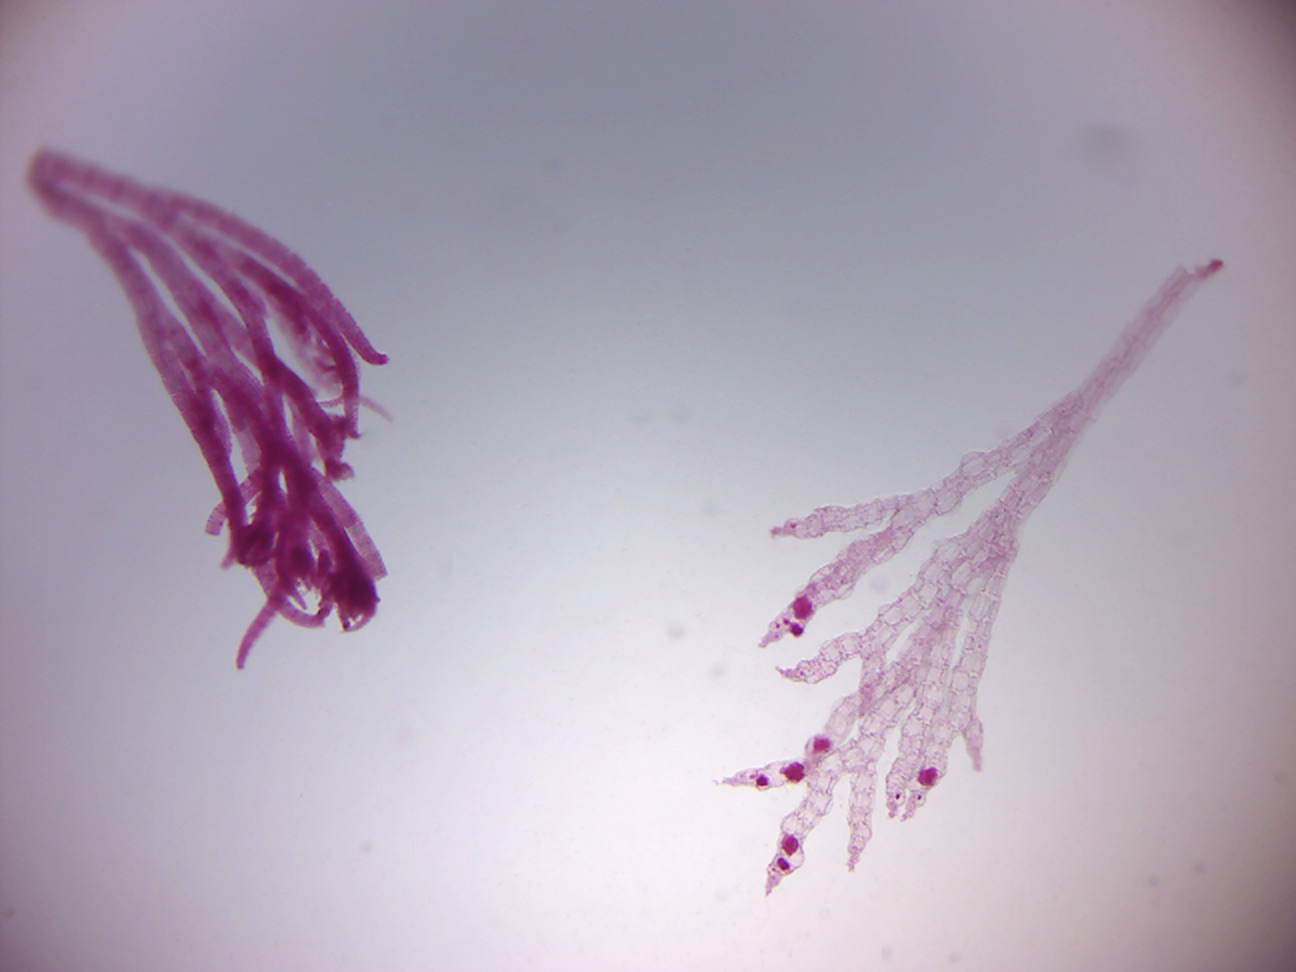
\includegraphics[width=0.7\linewidth]{./figures/protists/Polysiphonia_prepared} 

}

\caption{Polysiphonia.}\label{fig:polysiphonia}
\end{figure}

\subsection{\texorpdfstring{\emph{Stemonitis}}{Stemonitis}}\label{stemonitis}

\href{https://en.wikipedia.org/wiki/Stemonitis}{\emph{Stemonitis}}
(Figure \ref{fig:stemonitis}) is a distinctive genus of slime moulds
found throughout the world (except Antarctica). They are characterized
by the tall brown sporangia, supported on slender stalks, which grow in
clusters on rotting wood.

\begin{figure}

{\centering 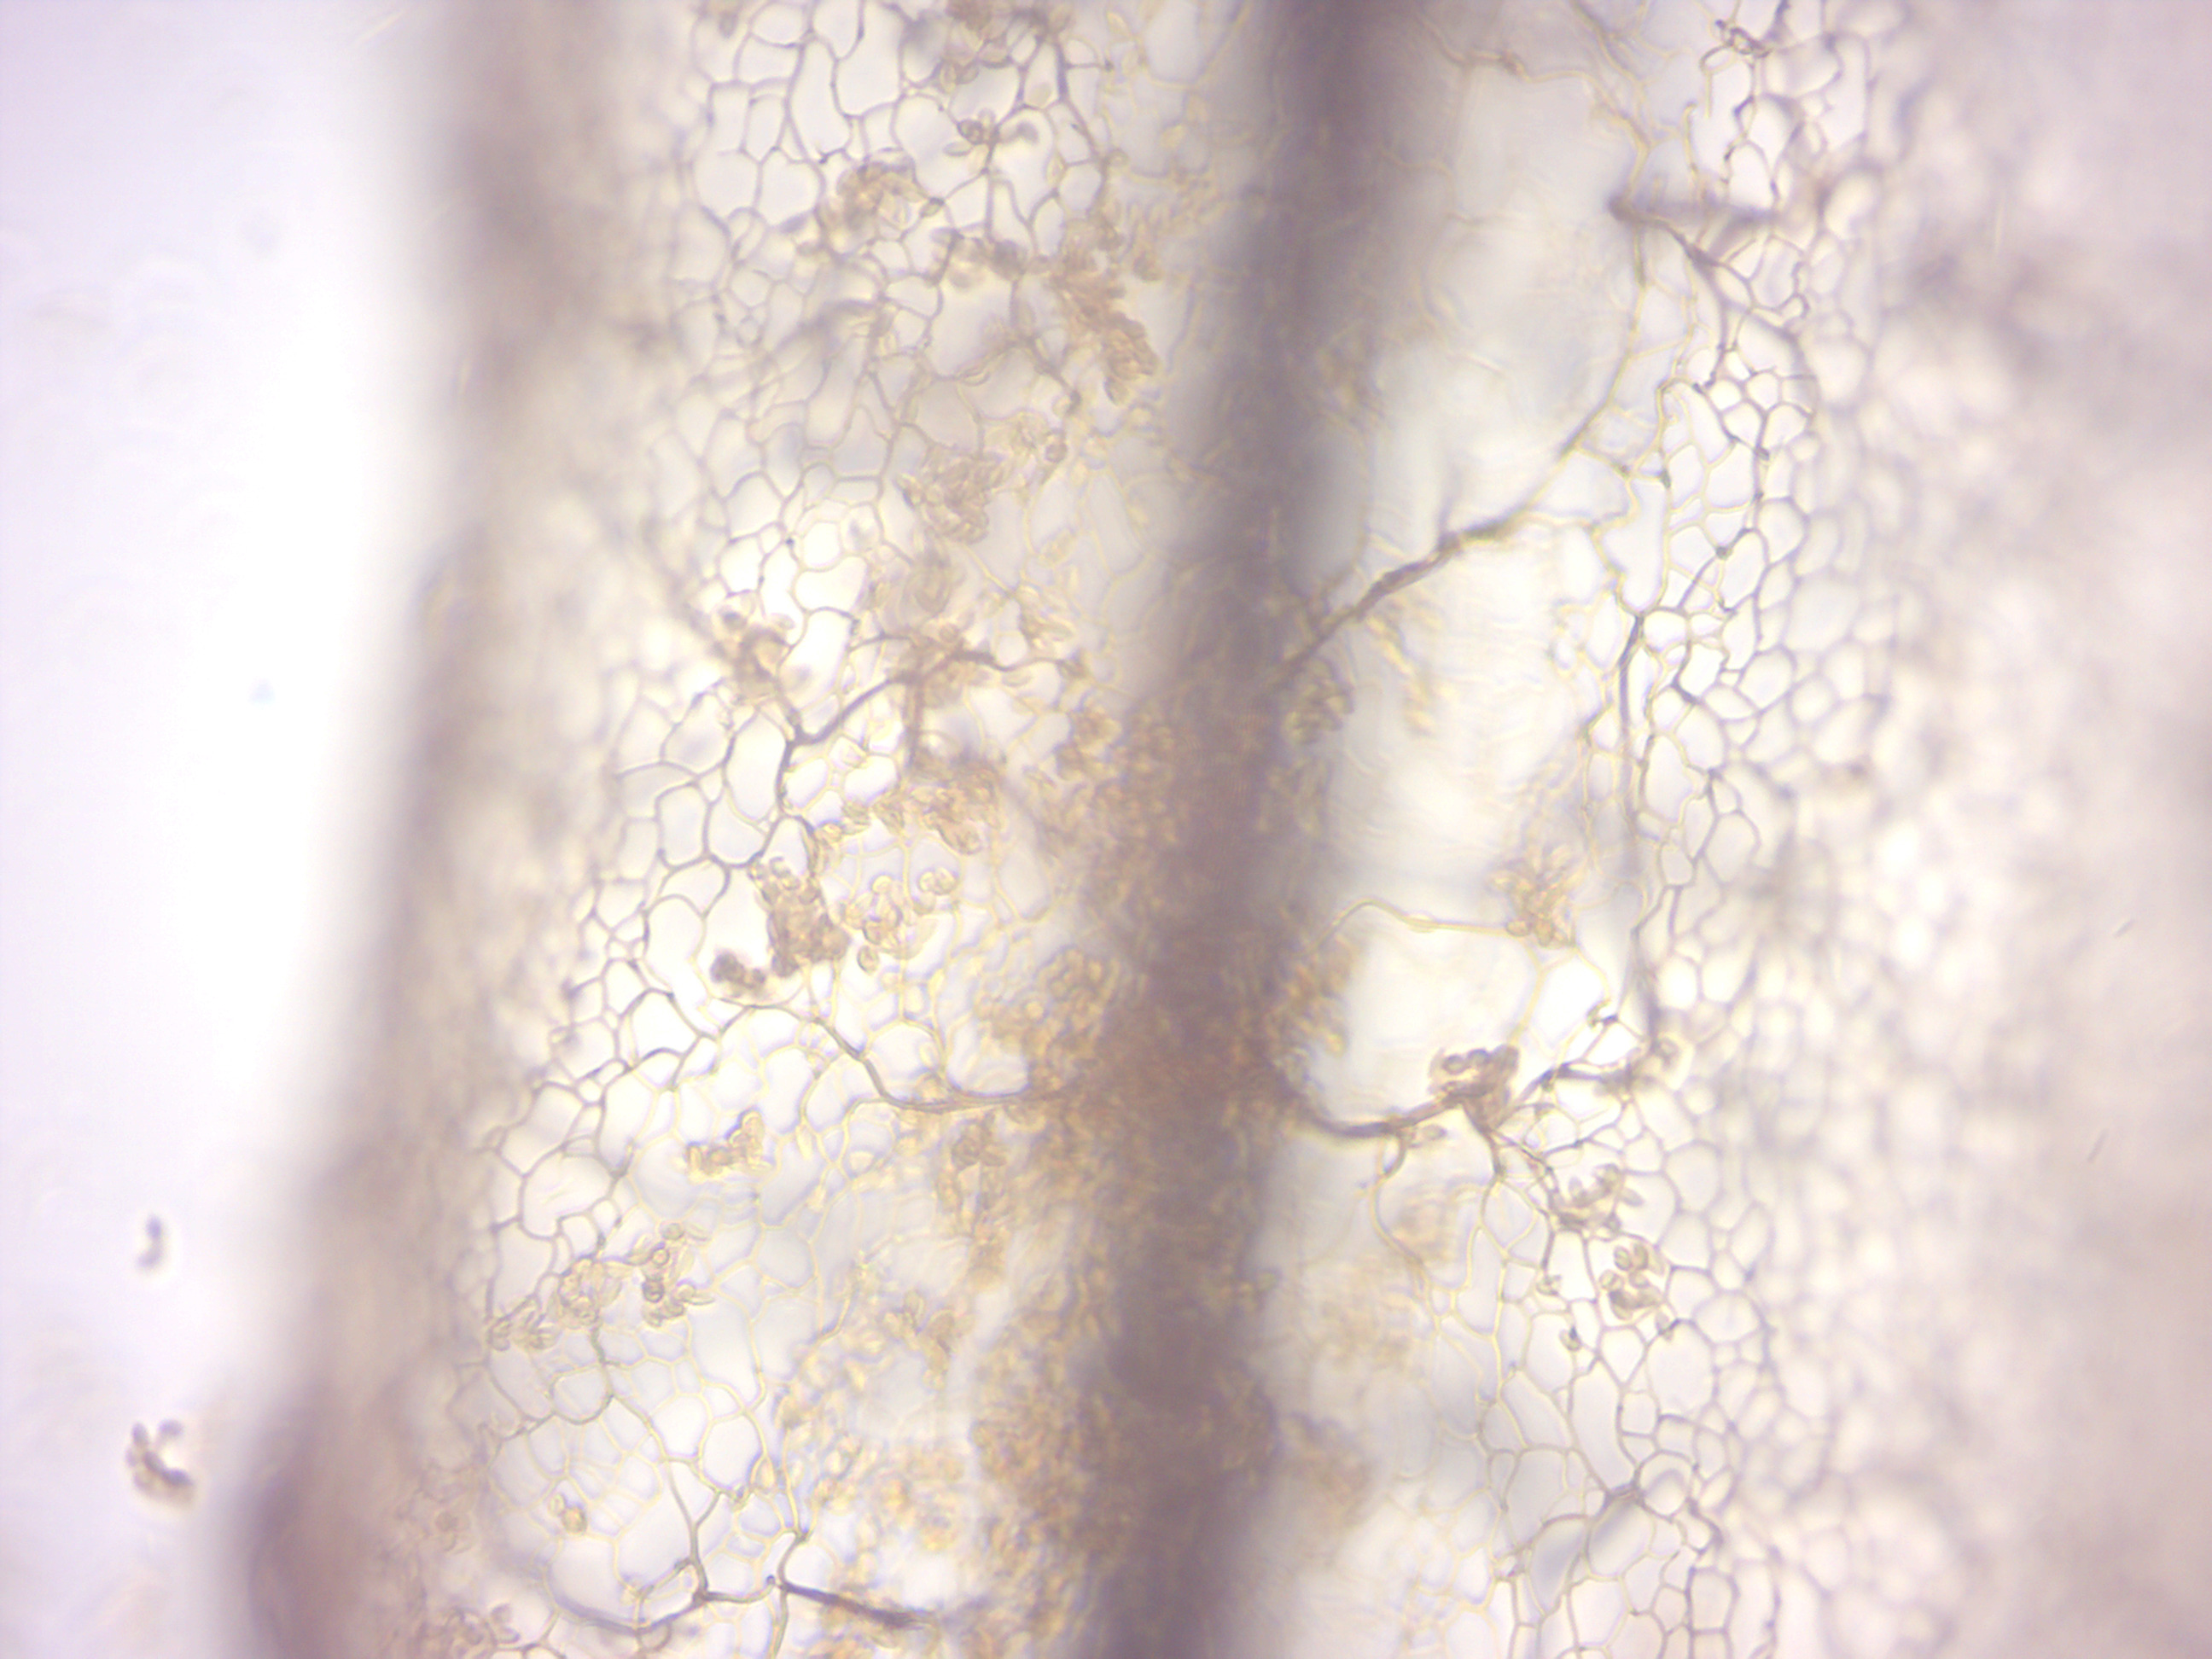
\includegraphics[width=0.7\linewidth]{./figures/protists/stemonitis} 

}

\caption{Stemonitis.}\label{fig:stemonitis}
\end{figure}

\subsection{\texorpdfstring{\emph{Saprolegnia}}{Saprolegnia}}\label{saprolegnia}

\href{https://en.wikipedia.org/wiki/Saprolegnia}{\emph{Saprolegnia}}
(Figure \ref{fig:saprolegnia}) is both a saprotroph and necrotroph.
Typically feeding on waste from fish or other dead cells, they will also
take advantage of creatures that have been injured. An infection is
known as oomycosis Saprolegnia is tolerant to a wide range of
temperature, 3 °C to 33 °C, but is more prevalent in lower temperatures.
While it is found most frequently in freshwater, it will also tolerate
brackish water and even moist soil. Saprolegnia filaments (hyphae) are
long with rounded ends, containing the zoospores. Saprolegnia generally
travels in colonies consisting of one or more species. They first form a
mass of individual hyphae. When the mass of hyphae grows large enough in
size to be seen without use of a microscope, it can be called a
mycelium.

\begin{figure}

{\centering 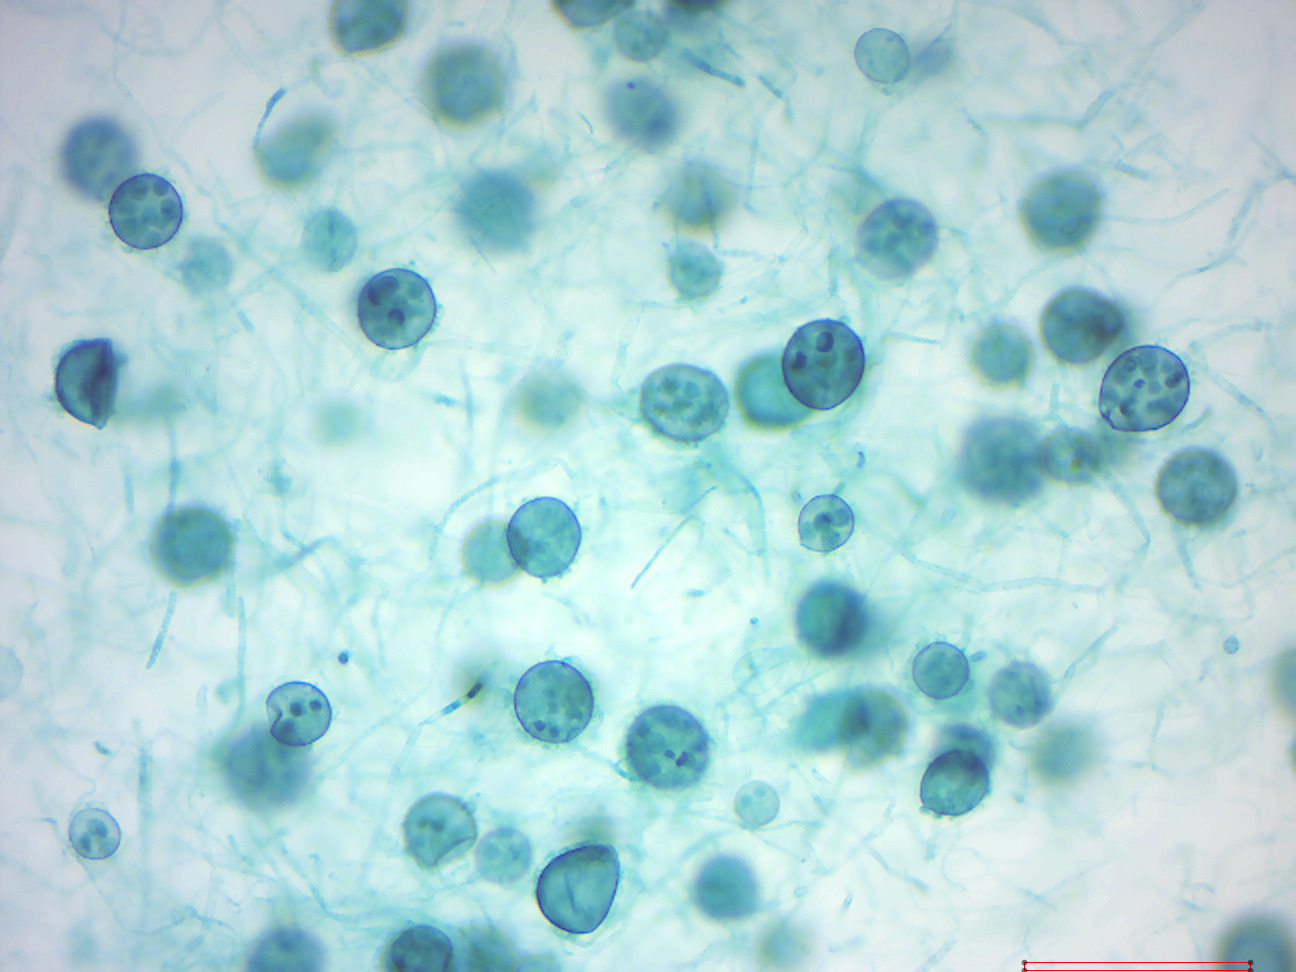
\includegraphics[width=0.7\linewidth]{./figures/protists/saprolegnia} 

}

\caption{Saprolegnia.}\label{fig:saprolegnia}
\end{figure}

It has a diploid life cycle which includes both sexual and asexual
reproduction. In the asexual phase, a spore of Saprolegnia releases
zoospores. Within a few minutes, this zoospore will encyst, germinate
and release another zoospore. This second zoospore has a longer cycle
during which most dispersal happens; it will continue to encyst and
release a new spore in a process called polyplanetism until it finds a
suitable substrate. When a suitable medium is located, the hairs
surrounding the spore will lock onto the substrate so that the sexual
reproduction phase can start. It is also during this stage of
polyplanetism that the Saprolegnia are capable of causing infection; the
most pathogenic species have tiny hooks at the end of their hairs to
enhance their infectious ability. Once firmly attached, sexual
reproduction begins with the production of male and female gametangium,
antheridia and oogonium respectively. These unite and fuse together via
fertilization tubes. The zygote produced is named an oospore.

\section{Review Questions}\label{review-questions-10}

\begin{enumerate}
\def\labelenumi{\arabic{enumi}.}
\tightlist
\item
  What are protists?
\item
  What are ciliata?
\item
  What are flagellata?
\item
  How do amoeba move?
\item
  What are slime molds?
\end{enumerate}


